\documentclass[twoside,fontsize=12pt,titlepage]{scrbook}

% * Packages
\usepackage[utf8]{inputenc}
\usepackage{graphicx}
\usepackage{eso-pic}
\usepackage[hidelinks]{hyperref}
\usepackage{natbib}
\bibliographystyle{apalike}
\usepackage{color, soul}
\usepackage{xcolor}
\usepackage{pdfpages}
\usepackage{ebgaramond}
\usepackage{nth}

% Show labels in pdf, remove for final
% \usepackage{showlabels}

\usepackage{gensymb}
\usepackage{makecell}
\usepackage{booktabs}
\usepackage{tabularx}

% glossary
\usepackage[xindy]{glossaries} 
\newglossaryentry{domain-knowledge}{%
  name={domain knowledge},%
  description={valid knowledge used to refer to an area of human endeavour, an autonomous computer activity, or other specialized discipline}}

\newacronym[description={(Environmental Noise Directive) \emph{DIRECTIVE 2002/49/EC OF THE EUROPEAN PARLIAMENT AND OF THE COUNCIL of 25 June 2002 relating to the assessment and management of environmental noise}. Policy directive within the EU setting out priorities and requirements of member nations for ensuring health and environmental protection as it relates to noise. Incorporates requirements for agglomerations to produce noise maps and identify and preserve quiet areas.}]{end}{END}{Environmental Noise Directive}

\newglossaryentry{isopl}{name={ISOPleasant},description={The value along the primary pleasantness dimension of the soundscape circumplex, calculated via a trigonometric projection of the other \gls{paq}s, as defined in \citet{ISO12913_3_2019IOS}}}

\newglossaryentry{isoev}{name={ISOEventful},description={The value along the primary eventfulness dimension of the soundscape circumplex, calculated via a trigonometric projection of the other \gls{paq}s, as defined in \citet{ISO12913_3_2019IOS}}}

% Psychoacoustic features
%TODO: Write descriptions of psychoacoustic features
\newglossaryentry{laeq}{name={$L_{Aeq}$},description={}}
\newglossaryentry{n5}{name={$N_{5}$},description={Psychoacoustic Loudness}}
\newglossaryentry{s}{name={$S$},description={Psychoacoustic Sharpness}}
\newglossaryentry{r}{name={$R$},description={Psychoacoustic Roughness}}
\newglossaryentry{iu}{name={$I$},description={Impulsiveness}}
\newglossaryentry{fs}{name={$FS$},description={Fluctuation Strength}}
\newglossaryentry{tu}{name={$T$},description={Tonality}}
\newglossaryentry{pa}{name={$PA$},description={Zwicker Psychoacoustic Annoyance}}
\newglossaryentry{la10la90}{name={$L_{A10}-L_{A90}$},description={}}
\newglossaryentry{la10}{name={$L_{A10}$},description={}}
\newglossaryentry{la90}{name={$L_{A90}$},description={}}

\newglossaryentry{lcla}{name={$L_{Ceq}-L_{Aeq}$},description={}}
\newglossaryentry{ra}{name={$RA$},description={Relative Approach}}

\newglossaryentry{environmental-unit}{
  name={environmental unit},
  description={An area within a public space in which environmental factors are consistent and which is typically perceived to constitute a single distinct area.}
}


\newacronym{ssid}{SSID}{Soundscape Indices}
\newacronym{satp}{SATP}{Soundscape Attributes Translation Project}
\newacronym{isd}{ISD}{International Soundscape Database}
\newacronym{wsp}{WSP}{World Soundscape Project}
\newacronym{iso}{ISO}{International Organization for Standardization}
\newacronym{covid19}{COVID-19}{Coronavirus disease of 2019}
\newacronym{slm}{SLM}{Sound Level Meter}
\newacronym{amb}{AMB}{Ambisonic recording}
\newacronym{bin}{BIN}{Binaural}
\newacronym{pic}{PIC}{Site pictures}
\newacronym{vid}{VID}{360\degree Video}
\newacronym{env}{ENV}{Environmental factors}
\newacronym{que}{QUE}{Questionnaires}
\newacronym{ssqp}{SSQP}{Swedish Soundscape Quality Protocol}
\newacronym{paq}{PAQ}{Perceived Affective Quality}
\newacronym{who5}{WHO-5}{WHO-5 Well-being Index}
\newacronym{vr}{VR}{Virtual Reality}
\newacronym{aic}{AIC}{Akaike Information Criterion}
\newacronym{vif}{VIF}{Variance Inflation Factor}
\newacronym{mae}{MAE}{Mean Absolute Error}
\newacronym{wasn}{WASN}{Wireless Acoustic Sensor Network}
\newacronym{rtn}{RTN}{Road Traffic Noise}
\newacronym{ane}{ANE}{Anomalous Noise Event}
\newacronym{complx}{COMPLX}{complex}
\newacronym{mushra}{MUSHRA}{MUlti Stimulus test with Hidden Reference and Anchor}
\newacronym{mlm}{MLM}{Multi-Level Model}
\newacronym[]{pca}{PCA}{Principal Components Analysis}
\newacronym{lmer}{LMER}{Linear Mixed-Effects Regression}
\newacronym{anova}{ANOVA}{ANalysis Of VAriance}
\newacronym{sns}{SNS}{Sympathetic Nervous System}
\newacronym{psns}{PSNS}{Parasympathetic Nervous System}
\newacronym{ans}{ANS}{Auditory Nervous System}
\newacronym{pns}{PNS}{Peripheral Nervous System}
\newacronym{art}{ART}{Attention Restoration Theory}
\newacronym[]{cns}{CNS}{Central Nervous System}
\newacronym[]{sem}{SEM}{Structural Equation Modelling}
\newacronym[]{ci}{CI}{confidence interval}
\newacronym[]{icc}{ICC}{intraclass correlation coefficient}
\newacronym[]{foi}{FOI}{features of interest}
\setacronymstyle{long-short}
\makeglossaries

% markup commands
\newcommand{\remark}[3]{%
    {\colorbox{#2}{\sffamily\scriptsize\bfseries\textcolor{white}{#1}}}
    {\sffamily\small\itshape\textcolor{#2}{#3}}
}
\newcommand{\misc}[1]{\remark{misc}{green}{#1}}
\newcommand{\draft}[1]{\remark{draft}{blue}{#1}}
\newcommand{\error}[1]{\remark{err}{red}{#1}}
\newcommand{\proof}[1]{\remark{proof}{orange}{#1}}
\newcommand{\cit}[1]{\remark{cit}{brown}{#1}}

% * Formatting
% Margins at the binding edge must not be less than 40mm (1.5 inches) and other margins not less than 20mm (0.75 inches).
% Double or one-and-a-half spacing should be used in typescripts except for indented quotations or footnotes where single spacing may be used.
\usepackage[a4paper,margin=20mm, bindingoffset=20mm, footskip=1cm]{geometry}
\usepackage[onehalfspacing]{setspace}
\AddToShipoutPicture*
{%
\put(0,730)% the specific point of the page with coordinates (x=100,y=100)
{
\includegraphics[scale=1]{Figures/UCL header.png}}%
}

\usepackage[capitalise]{cleveref}


%%%%%%%%%%%%%%%%%%%%%%%%%%%%%%%%%%%%%%%%%%%%%%%%%%%%%%%%%%%%%%%%%%%%%%%%%%%%%%%%%%%%%%%%%%%%%%%%%%

\begin{document}

\frontmatter
\newgeometry{margin=20mm, bindingoffset=0mm}
\begin{titlepage}
      % The title page must bear the following:
      % - the officially-approved title of the thesis
      % - the candidates full name as registered
      % - the institution name 'UCL'
      % - the degree for which the thesis is submitted
      \AddToShipoutPicture*{}
      \begin{center}
            \vspace*{3cm}

            \Huge
            \textbf{Predictive Modelling of Complex Urban Soundscapes}

            \vspace{0.5cm}
            \LARGE
            % Thesis Subtitle
            Multi-level Regression and Deep Learning Approaches

            \vspace{1.5cm}

            \textbf{Andrew James Mitchell}

            \vfill
            A thesis presented for the degree of\\
            Doctor of Philosophy\\
            \rule[-.5cm]{0.5\textwidth}{1pt}

            \vspace{1.5cm}

            \Large
            Institute for Environmental Design \& Engineering\\
            University College London (UCL)\\
            \today

            \vspace{1cm}

            Principal Supervisor: Prof. Jian Kang\\
            Co-Supervisor: Dr. Phil Symonds

      \end{center}
\end{titlepage}


\restoregeometry

%%%%%%%%%%%%%%%%%%%%%%%%%%%%%%%%%%%%%%%%%%%%%%%%%%%%%%%%%%%%%%%%%%%%%%%%%%%%%%%%%%%%%%%%%%%%%%%%%%

\chapter*{Declaration}
% The title page should be followed by a signed declaration that the work presented in the thesis is the candidate's own:
I, Andrew Mitchell, confirm that the work presented in this thesis is my own. Where information has been derived from other sources, I confirm that this has been indicated in the thesis.

\chapter*{Abstract}
% The signed declaration should be followed by an abstract consisting of no more than 300 words
Urban noise pollution affects 80 million EU citizens with substantial impacts on public health which are not well addressed by conventional noise control methods. Traditional noise control methods typically limit their focus to the reduction of unwanted noise, ignoring the benefits of increasing positive sounds and remaining restricted by practical limitations of noise reduction. Modern approaches to achieve improved health outcomes and public satisfaction aim to incorporate the perception of an acoustic environment, an approach known as ‘Soundscape’.

When attempting to apply soundscape in practical applications, it is immediately apparent that a predictive model of the users’ perceptual response to the acoustic environment is necessary. Whether to determine the impact of a design change, or to integrate large scale data at neighbourhood and city levels, a mathematical model of the interacting factors forms a vital component of the implementation of the soundscape approach.

Previous soundscape research has demonstrated that perception of the acoustic environment, while primarily driven by sound level, is mediated heavily by non-acoustic factors which interact with the sound level, spectral information, and temporal acoustic behaviour in complex ways. The soundscape is influenced by several levels of factors: the immediate and long-term acoustic environment, other environmental factors (e.g. temperature, air quality), the physical / visual characteristics and type of space, and even cultural and country-level expectations. When approached in a predictive model context, the acoustic data must form the core components, but a coherent framework for describing how the influence of the acoustic factors is affected by non-acoustic factors is required.  Through the combination of in-person field questionnaires and multi-factor characterisation of the environment, my research will focus on building up the levels of analysis and, finally, on integrating these levels and factors into an overall soundscape predictive model which focusses on interpretability and potential for practical use.


\chapter*{Acknowledgements}
This research was funded by the European Research Council.

People to thank:
\begin{itemize}
      \item Prof Jian Kang
      \item Dr Francesco Aletta
      \item Dr Tin Oberman
      \item Dr Phil Symonds
      \item Ms Mercede Erfanian
      \item Ms Magdalena Kachlicka
      \item Mr Matteo Lionello
      \item Friends: Nicole Watson, Nick Wilson, Valentina
\end{itemize}

\chapter*{List of Studies}

This doctoral thesis is based on the following studies:

\paragraph*{}
\textbf{Mitchell, A.}, Oberman, T., Aletta, F., Erfanian, M., Kachlicka, M., Lionello, M., \& Kang, J. (2020) The Soundscape Indices (SSID) Protocol: A Method for Urban Soundscape Surveys -- Questionnaires with Acoustical and Contextual Information. \emph{Applied Sciences, 10} (7), 2397. \url{https://doi.org/10.3390/app10072397}

\paragraph*{}
Erfanian, M., \textbf{Mitchell, A. J.}, Kang, J., \& Aletta, F. (2019). The Psychophysiological Implications of Soundscape: A Systematic Review of Empirical Literature and a Research Agenda. \emph{International Journal of Environmental Research and Public Health, 16(19)}, 3533. https://doi.org/10.3390/ijerph16193533

\paragraph*{}
Erfanian, M., \textbf{Mitchell, A.}, Aletta, F., \& Kang, J. (2020). Psychological Well-being and Demographic Factors can Mediate Soundscape Pleasantness and Eventfulness: A large sample study. \emph{Environmental Psychology}.

\paragraph*{}
Orga, F., \textbf{Mitchell, A.}, Freixes, M., Aletta, F., Alsina-Pagès, R. M., \& Foraster, M. (2021). Multilevel Annoyance Modelling of Short Environmental Sound Recordings. \emph{Sustainability, 13}(11), Article 11. \url{https://doi.org/10.3390/su13115779}

\paragraph*{}
\textbf{Mitchell, A.}, Oberman, T., Kachlicka, M., Aletta, F., Lionello, M., Erfanian, M., \& Kang, J. (2021). Investigating Urban Soundscapes of the COVID-19 Lockdown: A predictive soundscape modelling approach. \emph{JASA}.

\paragraph*{}
\textbf{Mitchell, A.}, Soelitsyo, C., Erfanian, M., Xue, J-H., Oberman, T., Kang, J., \& Aletta, F. (2021). A Temporal Convolutional Neural Network for Multi-label Sound Recognition and Annoyance Detection of Complex Soundscapes. \emph{IEEE}.

\paragraph*{}
\textbf{Mitchell, A.}, Aletta, F., Chalabi, Z., \& Kang, J. (2021). From Deterministic to Probabilistic Soundscapes: A critical tour around the soundscape circumplex. \emph{JASA-EL}.



%%%%%%%%%%%%%%%%%%%%%%%%%%%%%%%%%%%%%%%%%%%%%%%%%%%%%%%%%%%%%%%%%%%%%%%%%%%%%%%%%%%%%%%%%%%

\newpage
The following studies are related works which influenced this thesis and were completed as part of the same work but have not been included as key components:

\paragraph*{}
Kang, J., Aletta, F., Oberman, T., \textbf{Mitchell, A}., Erfanian, M., Tong, H., Torresin, S., Xu, C., Yang, T. (2021). Supportive Soundscapes are Crucial for Sustainable Cities and Communities. \emph{Nature Sustainability}.

\paragraph*{}Lionello, M., Aletta, F., \textbf{Mitchell, A.}, \& Kang, J. (2020). Introducing a Method for Intervals Correction on Multiple Likert Scales: A Case Study on an Urban Soundscape Data Collection Instrument. \emph{frontiers in Psychology}.

\paragraph*{}Aletta, F., Oberman, T., \textbf{Mitchell, A.}, Tong, H., \& Kang, J. (2020). Assessing the changing urban sound environment during the COVID-19 lockdown period using short-term acoustic measurements. \emph{Noise Mapping}.

% \paragraph*{}Tong, H., Aletta, F., \textbf{Mitchell, A.}, Oberman, T., \& Kang, J. (2021). Increases in noise complaints during the COVID-19 lockdown in Spring 2020: A case study in Greater London, UK. \emph{Science of the Total Environment}.

%%%%%%%%%%%%%%%%%%%%%%%%%%%%%%%%%%%%%%%%%%%%%%%%%%%%%%%%%%%%%%%%%%%%%%%%%%%%%%%%%%%%%%%%%%%%%%%%%%

\chapter*{Impact Statement}
% The abstract should be followed by an impact statement consisting of no more than 500 words.
The statement should describe, in no more than 500 words, how the expertise, knowledge, analysis, discovery or insight presented in your thesis could be put to a beneficial use. Consider benefits from \textbf{inside} and \textbf{outside} academia and the ways in which these benefits could be brought about.

\chapter*{COVID-19 Statement}

In March of 2020, 18 months into the development of this thesis, the COVID-19 pandemic hit the UK, forcing it into lockdowns which would continue for over a year. Solely by good fortune and a tendency to speed ahead with too-little thought, the primary data collection had fortunately been completed prior to the first lockdown. However, this work was impacted in three ways:

\begin{enumerate}
      \item Further in-situ data collection could not be completed, reducing the range of soundscape types we could include;
      \item The unprecedented and stressful world of the pandemic had a significant mental health and social impact, the effects of which cannot be quantified, nor overstated;
      \item In response to the unique scientific opportunity of a world-wide transportation and social lockdown, new, unplanned studies were carried out.
\end{enumerate}

In particular, this final point has had an impact on the structure and content of this thesis. Certain aspects of the research, in particular the model development and building, were accelerated and put into practice to investigate the impacts of the COVID lockdowns, before being returned to and further developed. The initial research plan would have followed a more logical path of nailing down the model development first, then moving on to a first implementation. In addition, new work was added to this thesis which may appear incongruous or unrelated, but represents a great deal of necessary work which further informed the key strains of the thesis.

%%%%%%%%%%%%%%%%%%%%%%%%%%%%%%%%%%%%%%%%%%%%%%%%%%%%%%%%%%%%%%%%%%%%%%%%%%%%%%%%%%%%%%%%%%%%%%%%%%

\tableofcontents
% In each copy of the thesis the abstract should be followed by a full table of contents (including any material not bound in) and a list of tables, photographs and any other materials.

\listoffigures
\listoftables

%%%%%%%%%%%%%%%%%%%%%%%%%%%%%%%%%%%%%%%%%%%%%%%%%%%%%%%%%%%%%%%%%%%%%%%%%%%%%%%%%%%%%%%%%%%%%%%%%%%%

\mainmatter

\chapter{Introduction}
\label{ch:intro}

\section{Research Summary}
Urban noise pollution affects 80 million EU citizens with substantial impacts on public health which are not well addressed by conventional noise control methods. Traditional noise control methods have typically limited their focus to the reduction of unwanted noise, ignoring the potential benefits of increasing positive sounds and remaining restricted by practical limitations of noise reduction. Modern approaches to achieve improved health outcomes and public satisfaction aim to incorporate a person's perception of an acoustic environment, an approach known as 'Soundscape'.

Soundscape studies strive to understand the perception of a sound environment, in context, including acoustic, (non-acoustic) environmental, contextual, and personal factors. These factors combine together to form a person's soundscape in complex interacting ways \citep{Berglund2006Tool}. In order to predict how people would perceive an acoustic environment, it is essential to identify the underlying acoustic and non-acoustic properties of soundscape.

% From: Upgrade report
When attempting to apply soundscape in practical applications in the built environment, it is immediately apparent that a predictive model of the users' perceptual response to the acoustic environment is necessary. Whether to determine the impact of a design change, or to integrate a large scale data at neighbourhood and city levels, a mathematical model of the interacting factors will form a vital component of the implementation of the soundscape approach. This work is intended to identify methods for incorporating contextual and objective information into a useable and interpretable predictive model of urban soundscapes. In order to achieve this, a protocol for collecting the multi-level, multi-factor perceptual assessment data has been developed and implemented, resulting in a large soundscape database. Several avenues of investigation are then drawn from the database and addressed throughout this thesis. The primary research questions are:

% TODO: Try to move this to the end of the introduction.
\begin{enumerate}
  \item What are the primary acoustic features involved in soundscape formation and what are the driving interactions between acoustic features and soundscape assessment?
  \item How does the sound source composition in a complex sound environment mediate this interaction and how can this effect be simplified and modelled?
  \item How can the multiple levels of soundscape formation be simplified and integrated into a cohesive predictive model, and what interpretations about the cross-effects of these levels can be drawn from the model?
  \item In what ways and to what extent can predictive soundscape modelling be applied to address future urban design challenges? How can these methods best be integrated into policy, design, noise mapping, and engineering practice?
\end{enumerate}

Towards answering these questions, the results of five %TODO: check this number at the end.
peer-reviewed studies are presented. These studies represent a series of work to 

\begin{enumerate}
  \item Advance the conceptual development and practice of soundscape studies
  \item Develop a transparent and useful method of predicting soundscape assessments
  \item Investigate the various components which influence soundscape perception, including personal factors like psychological well-being, acoustical factors, and sound source specifics and to integrate these components into the predictive modelling methods.
\end{enumerate}

\section{The SSID Project}
The \gls{ssid} Project is a five-year, multi-disciplinary project funded by a Horizon 2020 European Research Council grant (no. 740696).

\subsection{Project collaborators}

\subsection{Motivation for the SSID Project}

\section{Research Aims}

\section{Soundscape Indices and Metrics}

\section{General Aim}


\chapter{Literature Review}
\label{ch:lit}

\section{Impact of Urban Noise on Health and Wellbeing}

\cit{Environmental noise in Europe 2020}

\hl{Give a full formal background to why noise control is important for public health}.
% https://www.euro.who.int/__data/assets/pdf_file/0008/383921/noise-guidelines-eng.pdf?ua=1

\section{Current Methods of Assessing and Addressing Urban Noise}

The approach to a practical predictive soundscape model arrived at within this thesis is heavily based on past environmental acoustics approaches. I will therefore begin with a brief summary of these past approaches.

\subsection{Acoustical Parameters}

\subsection{ISO Environmental Acoustics Standards}
\hl{ISO 1996-1, esp sections on annoyance, e.g. Annex F, G, H}

\subsection{EU Noise Mapping}

\cit{Environmental noise in Europe 2020}

\subsection{Shortcomings}


\section{Soundscape Studies}

\subsection{Soundscape Descriptors and Indices}

\subsection{World Soundscape Project}

\subsection{Swedish Soundscape Quality Protocol}


\subsection{Demographic differences}
Several studies have attempted to study the degree to which personal and demographic factors influence a person's soundscape perception. In some conceptions \cit{Kou2020effects} % CITE add Erfanian 2020
these personal factors are classed as 'contextual' soundscape indicators - features which influence or, in a modelling context, be used as independent variables to predict the value of a soundscape descriptor. The personal factors help to create a personal soundscape interpretation model which is individual to each person.

In this way, a person's individual state-of-mind, ethnic identity, educational background, gender identity, etc. form a pseudo-deterministic framework %! what a load of crap
through which the physical inputs from their environment are filtered. Clearly, many of these personal factors could never be measured and even those which are measurable will have wide ranges of legitimate effects, however estimating the degree and type of effect they may have can both help us better predict individual soundscape assessments and understand how group identities influence sound perception.

%TODO: Need to include earlier, more foundational studies into demographic factors

\paragraph*{Section on Erfanian et al. 2020, Psychological Well-being}

\paragraph*{Low-income and minority evidence} % FIXME I think this section will need to be heavily revised for phrasing and content. I'm not happy with how I'm discussing under-represented groups.
A consistent limitation of soundscape studies investigating the influence of personal factors is a sampling bias towards majority ethnicities (typically White British for UK studies and ethnic Chinese for Chinese studies) and middle-class and highly educated groups. % CITE Hoo boy citation definitely needed
This results in not only incomplete information about how demographics influence soundscape perception, but also represents a systemic under-representation of certain environments. While it may be unclear to what extent ethnicity and social class internally influence a person's perception, it is clear that these groups are exposed to different sound environments % NOTE: socio-economic studies - Huan 2019? Jian ~2015?, Environmental noise in Europe 2020

and therefore studies which do not include under-represented groups are also by definition not including those sound environments which those groups inhabit.

A recent study by \cit{Kou2020effects} was successful in making inroads in these under-represented environments by studying the Humboldt Park neighbourhood in Chicago, USA. Their study included
% TODO: Finish summarising results from Kou2020


\section{Approaches to Soundscape in Engineering}

From this literature review, some conclusions about current approaches to incorporating the concept of "soundscape" into practical engineering and architectural design have been identified.

\subsection{The Quiet Areas approach}

This approach maintains a focus on "identifying and preserving quiet areas" \cit{Environmental noise in Europe 2020} following the imperative given in the Environmental Noise Directive \cit{END}. This approach is mostly rooted in a noise mindset, although the methods employed for identifying quiet areas varies across countries within the EEA. Background sound levels seem to play an important role in identifying quiet areas, in particular when attempting to

%TODO Continue adding from Remarkable notes

\section{Existing Predictive Models}

Contrary to the hopes expressed by \citet{Aletta2014Towards}, that "ideally there should be one acoustic indicator per dimension", the evidence from subsequent investigations and modelling attempts \citep{Lionello2020systematic} indicates this to be unlikely. There appears to be no reason we should think the perceptual dimensions should be reduced to a single acoustic indicator. The dimensions of soundscape represent complex perceptual concepts which we should expect to be composed of a multi-factor interaction between the input features. This necessary complexity  highlights the need for a more sophisticated machine learning approach in order to handle and interpret the interactions between the many input features which contribute to the formation of a soundscape perception.
\citep{Aletta2016Soundscape}

\citep{Lionello2020systematic}

\subsection{Models based on non-acoustic data sources}

\citep{Verma2020Predicting}, \citep{Gasco2020Social}


\chapter{Methods}
\label{chap:methods}

%%%%%%%%%%%%%%%%%%%%%%%%%%%%%
%FIXME: Find a better spot for this
The ability to predict the likely soundscape assessment of a space is crucial to implementing the soundscape concept in practical design. Current methods of assessing soundscapes are generally limited to a post-hoc assessment of the existing environment, where users of the space in question are surveyed regarding their experience of the acoustic environment \citep{Engel2018Review, Zhang2018Effect}. While this approach has proved useful in identifying the impacts of an existing environment, designers require the ability to predict how a change or proposed design will impact the soundscape of the space. To this end, a model that is built upon measurable or estimate-able quantities of the environment would represent a leap forward in the ability to design soundscapes.

\section{Questionnaires}

 The full protocol developed for this thesis is outlined in Chapter \ref{chap:protocol}. The development and presentation of this protocol involved a substantial development and testing phase, and represents a novel advancement in soundscape survey methodology. Therefore it was submitted and published as a peer-reviewed journal article in MDPI Applied Sciences as \citet{Mitchell2020Soundscape} and is presented as a stand-alone chapter within this thesis.

 \subsection{Likert Responses}

 \subsection{Circumplex Projection}

\section{Psychoacoustics and Auditory Perception}

 \subsection{Psychoacoustic Parameters}

   \subsubsection{Loudness}
   \emph{Zwicker and Fastl, Chap 8, see Mendeley notes and python-acoustics development notes.}
 \subsection{Feature Selection}

\section{Machine Learning and Regression Techniques}

 \subsection{Feature Selection}
   \subsubsection{Mutual Information}
   \draft{It appears that mutual information is related to the Bayes formula. I still need to read more into this, but it appears based on relative and overlapping probability distributions between the variables in question.}
   \paragraph*{From scholarpedia:}
   % http://www.scholarpedia.org/article/Mutual_information
   \draft{Based on entropy, where the uncertainty about a variable can be expressed as "the number of yes/no questions it takes to guess a random variable, given knowledge of the underlying distribution and taking the optimal question-asking strategy". "The mutual information is therefore the \emph{reduction} in uncertainty about variable $X$, or the expected reduction in the number of yes/no questions needed to guess $X$ after observing $Y$.". }

   \draft{"Mutual Information is just one way among many of measuring how related two variables are. However, it is a measure ideally suited for analyzing communication channels. Abstractly, a communication channel can be visualized as a transmission medium which receives an input $x$ and produces an output $y$. If the channel is \emph{noiseless}, the output will be equal to the input. However, in general, the transmission medium is noisy and an input $x$ is converted to an output $y$ with probability $P_{Y|X}(y|x)$. }
   \misc{This seems very useful for my conception of sound perception / auditory processing, where the perception system is a noisy communication channel.}

   \subsubsection{Conditional Mutual Information}
   The Mutual Information between two variables, given another variable as a control.

 \subsection{Clustering Analysis}
   \paragraph{K-means}
   \paragraph{nbclust}

 \subsection{Modelling Likert-type Data}

   \subsubsection{Multiple Linear Regression}

   \subsubsection{Ordinal Logistic Regression}

   \subsubsection{Multi-output Regression}

 \subsection{Multi-level Models}

 \subsection{Bayesian Regression}


\chapter[The SSID Protocol]{The Soundscape Indices (SSID) Protocol: A Method for Urban Soundscape Surveys -- Questionnaires with Acoustical and Contextual Information}

\label{chap:protocol}

%TODO: Still need to fix tables
%TODO: Add in citations
%TODO: Edit intro / add context of this being a stand-alone scientific work.

Conducting urban soundscape studies on a scale large enough to form a machine learning dataset presents a unique challenge. The standardised methods of conducting soundscape surveys \citep{ISO12913_2_2018IOS} are labour-intensive, time-consuming, and provide limited information about the acoustical and environmental context.

\section*{Abstract}

 A protocol for characterizing urban soundscapes for use in the design of \gls{ssid} and general urban research as implemented under the European Research Council (ERC)-funded SSID project is described in detail. The protocol consists of two stages: (1) a Recording Stage to collect audio-visual recordings for further analysis and for use in laboratory experiments, and (2) a Questionnaire Stage to collect in-situ soundscape assessments via a questionnaire method paired with acoustic data collection. Key adjustments and improvements have been made to enable the collation of data gathered from research groups around the world. The data collected under this protocol will form a large-scale, international soundscape database.

\section{Introduction}
 %NOTE: This intro might work better to form the thesis intro. Then jump into the protocol at "Purpose" and design

 %NOTE: Could replace with an intro which ends up justifying the development of the protocol as its own stand-alone scientific work.

 Soundscape studies strive to understand the perception of a sound environment, in context, including acoustic, (non-acoustic) environmental, contextual, and persona factors. These factors combine together to form a person's soundscape in complex interacting ways \cit{1}. In order to predict how people would perceive an acoustic environment, it is essential to identify the underlying acoustic and non-acoustic properties of soundscape.

 The soundscape community is undergoing a period of increased methodological standardisation in order to better coordinate and communicate the findings of the field. This process has resulted in many operational tools designed to assess and understand how sound environments are perceived and apply this to shape modern noise control engineering approaches. Important topics which have been identified throughout this process are soundscape 'descriptors', 'indicators', and 'indices'. \citet{Aletta2016Soundscape} defined soundscape descriptors as "measures of how people perceive the acoustic environment"; soundscape indicators as "measures used to predict the value of a soundscape descriptor"; and soundscape indices can then be defined as "single value scales derived from either descriptors or indicators that allow for comparison across soundscapes" \citep{Aletta2018Towards}.

 This conception has recently been formalised and expanded upon with the adoption of the recent ISO 12913 standard series \citep{ISO12913_1_2014IOS,ISO12913_2_2018IOS,ISO12913_3_2019IOS}. ISO 12913 Part 1 sets out the definition and conception of Soundscape, defining it as the "acoustic environment as perceived or experienced and / or understood by a person or people, in context". Here, the soundscape is separated from the idea of an acoustic environment, which encompasses all of the sound which is experienced by the receiver, including any acoustically modifying effects of the environment. In contrast, the soundscape considers the acoustic environment, but also considers the impact of non-acoustic elements, such as the listener's context and the visual setting, and how these interact with the acoustic environment to influence the listener's perception.

 The ISO/TS 12913-2:2018 is the current reference document addressing data collection and reporting requirements in soundscape studies. In terms of methods, the ISO document covers two main approaches, namely: soundwalks combined with questionnaires (Methods A and B) and narrative interviews (Method C) \citep{ISO12913_2_2018IOS}, which relate to on-site and off-site data collection, accordingly. Part 3 of the ISO 12913 series builds on Part 2 and provides guidelines for analysing data gathered using only those methods \citep{ISO12913_3_2019IOS}. However, the range of possible methodological approaches to soundscape data collection is much broader and it includes, for instance, laboratory experiments \citep{Aletta2016Soundscape,Sun2019Classification,Oberman2018Towards}, pseudo-randomized experience sampling \citep{Craig2017Experience}, and even non-participatory studies \citep{Lavia2018Non}. The protocol described in this paper was designed having in mind the need for a relatively large soundscape dataset that could be used for design and modelling purposes, thus trying to expand the scope of soundwalks that typically deal with much smaller samples of participants \citep{Engel2018Review}. For the sake of comparability and standardization with these methods, we chose to refer to the soundscape attributes reported in the ISO Part 2 (Method A).

 Several studies prior to the formalisation of the ISO standards on soundscape demonstrated the general, but inadequate, relationship between traditional acoustic metrics, such as $L_{Aeq}$, with the subjective evaluation of the soundscape \cit{1, 12-15}. These have typically aimed to address the existing gap between traditional environmental acoustics metrics and the experience of the sound environment. \citep{Yang2005Acoustic} showed that, when the sound level is 'lower than a certain value, say 70 dB(A)', there is no longer a significant change in the evaluation of acoustic comfort as the sound level changes. However, the perceived sound level does continue to change along with the measured sound level, showing that (1) measured sound level is not enough to predict soundscape descriptors such as 'acoustic comfort', and (2) there is a complex relationship between perceived sound level and soundscape descriptors which is mediated by other factors.

 % NOTE I've written this intro section in a few places. I'm going to move on to the protocol specific stuff and decide what to do with the above later.

\section{Purpose}

 The \gls{ssid} Protocol was designed to achieve two primary goals:
 \begin{enumerate}
   \item gather in-situ soundscape assessments from the public, which can be further analysed and utilised in designing a soundscape index;
   \item conduct recordings needed to reproduce the audio-visual environment of a location in a laboratory setting for conducting controlled experiments on soundscape.
 \end{enumerate}

 These two goals represent two levels of data required for developing a general soundscape model. The first enables large scale data collection, resulting in a database with thousands of perceptual responses and their corresponding quantitative data which can be statistically analysed on a large scale, or used for training in machine learning modelling. In-situ assessments also represent the most holistic assessment, ensuring all factors that influence the soundscape are present, including those which cannot be reproduced elsewhere.

 However, there are questions that cannot be practically addressed in-situ, such as soundscape assessment of less- or un-populated areas, the influence of mismatched acoustic and visual cues, physiological and neural responses to various soundscapes, and so on \cit{31}. Laboratory experiments with controlled environments are required to address these aspects. Toward the development of a coherent \gls{ssid}, therefore, it is important that these two forms of data are collected simultaneously and with compatible methods, such that the results of the two approaches can be confidently combined and compared. In addition, since this protocol is intended to be used for the creation of a large-scale international database with additions carried out by several different and remote teams, it has been designed for efficiency, scalability, and information redundancy.

\section{Protocol Design and Equipment}
 The first goal is achieved by conducting in-situ questionnaires using a slightly altered version of Method A (questionnaire) from Annex C of the ISO/TS 12913-2:2018 technical specification \citep{ISO12913_2_2018IOS} collected either via handheld tablets or paper copies of the questionnaire. Typically, a minimum of 100 responses are collected at each location during multiple 2-5 hr sessions over several days. During the survey sessions, acoustic data are collected via a stationary class 1 or class 2 \gls{slm} (as defined in IEC 61672-1:2013 \cit{IEC61672}) running throughout the survey period and through binaural recordings taken next to each respondent. These acoustic and response data are linked through an indexing system so that features of the acoustic environment can be correlated with individual responses or with the overall assessment of the soundscape, as required by researchers.

 The second goal is achieved by making First-Order (or higher) Ambisonic recordings simultaneously with 360\degree video which can be reproduced in a virtual reality environment. It has been shown that head-tracked binaural and multi-speaker ambisonic reproduction of recorded acoustic environments recorded in this way have high ecological validity \cit{33}, particularly when paired with simultaneous head-tracked virtual reality video \cit{22, 34, 35}.

 The on-site procedure to collect these data are separated into two stages, which will be outlined in detail in Section \ref{sec:proc}. The stage during which the audio-visual recordings are made for lab experiments is called the \textbf{Recording Stage}, while the stage during which questionnaires and environmental data are captured is called the \textbf{Questionnaire Stage}.

 The procedure has been designed to include multiple levels of data and metadata redundancy, making it robust to on-site issues and human error. The most crucial aspect of the redundancy is ensuring the perceptual responses can be matched with the appropriate corresponding environmental and acoustic data even when some information is lost or forgotten.

 \subsection{Labelling and Data Organisation}
   \label{section:metadata}
   In order to be able to identify all of the many data components of the Recording and Questionnaire Stages and to associate these with their various corresponding data, the following labelling system is suggested. This system is focussed on (1) relating all of the separate recordings and factors to specific questionnaire responses and (2) efficiency and consistency on site. A recent paper by \citet{Aumond2017Modeling} demonstrated the importance of addressing multiple levels of factors which influence perception, from individual-, to session-, to location-level. The successful pleasantness models built incorporating these information levels showed a marked improvement over the equivalent individual-level or location-level only models. The data organisation system proposed here was designed in order to maintain this important information, and the levels of information for the data collected on site are shown in Table \ref{tab:metadata}.

   At the top level is the \textbf{Location} information. This includes information about the location which does not change day-to-day, and generally characterises the architectural character of the space, or typical climate conditions for the area. As described in Section \ref{sec:loc-selection}, each '\gls{environmental-unit}' should be considered a new location. Therefore, if researchers want to investigate the differences in soundscape assessment in the middle of a small urban park and along the road next to the same park, these would be considered different locations since they would (typically) have different environmental factors and should be given difference names. The name chosen should be concise, but it should be obvious what location is referred to.

   The next level is information which is specific to each session, labelled with a \textbf{SessionID}. This SessionID should contain the name of the location and a numerical index which will increase with each repeated session at that location. The SessionID is associated with the data collected during the Recording Stage, and with the data which are continuous throughout the Questionnaire Stage, SLM, and ENV data. For easy automatic processing, correct spelling and consistency with the format is crucial so that data can be filtered according to the SessionID or the location, as is often necessary. In addition, for ease of automatic processing, it is recommended not to include spaces in the SessionID to avoid string splitting issues in analysis code.

   Underneath each SessionID will be a set of \textbf{GroupID}s. One GroupID is assigned for \emph{each group of participants}. This should correspond to a single binaural recording and a single 360\degree photo. This will be used to (1) relate multiple surveys taken simultaneously and (2) link the recording and photo with the surveys. The GroupID is particularly crucial as it allows commonly missing data to be shared across multiple collection methods. For instance, occasionally paper questionnaires will be missing start and end time information. In this case, this information can be pulled directly from other questionnaires with the same GroupID. Where no questionnaires have the times, it is possible to extract an approximate start time from the binaural recordings or 360\degree photo and then estimate an average end time.

   The GroupID should have the following format: [a set of letters representing the location name][the SessionID index number][an incrementing index for each group]. For example, for the second session at Regent's Park Japanese Garden, the location name is 'RegentsParkJapan', the GroupID letters might be 'RPJ'; the SessionID would be 'RegentsParkJapan2', so the GroupIDs for that session would start at '201'. Therefore, for example, the tenth group of participants for that session would be labelled 'RPJ210'. This format ensures that, if the location or SessionID are not recorded for a questionnaire, it is still obvious which session it belongs to.

   % Please add the following required packages to your document preamble:
   % \usepackage{booktabs}
   % \usepackage{graphicx}
   \begin{table}[]
     \centering
     \resizebox{\textwidth}{!}{%
       \begin{tabular}{@{}cclccccc@{}}
         \toprule
         \textbf{Level of information} & \multicolumn{6}{c}{\textbf{Example Label}} & \textbf{Factors measured at this level}                                                                                                                             \\ \midrule
         Location                      & \multicolumn{6}{c}{RegentsParkJapan}       & GPS, Architectural typology, visual openness, etc.                                                                                                                  \\ \midrule
         SessionID                     & \multicolumn{4}{|c|}{RegentsParkJapan1}    & \multicolumn{2}{c|}{RegentsParkJapan2}             & SLM, session notes, ENV                                                                                        \\ \midrule
         GroupID                       & \multicolumn{2}{|c|}{RPJ101}               & \multicolumn{1}{c|}{RPJ102}                        & \multicolumn{1}{c|}{...} & \multicolumn{1}{|c|}{RPJ201} & \multicolumn{1}{c|}{\ldots} & BIN, PIC               \\ \midrule
         Questionnaire                 & \multicolumn{2}{|c|}{1, 2, 3}              & \multicolumn{1}{c|}{4, 5}                          & \multicolumn{1}{c|}{...} & \multicolumn{1}{c|}{25, 26}  & \multicolumn{1}{c|}{\ldots} & QUE, Start \& End time \\ \bottomrule
       \end{tabular}%
     }
     \caption{Labelling system for on site data collection. Regents Park Japanese Garden is used as an example location. Abbreviations as defined in Table \ref{table:factors} - SLM: Sound Level Meter (acoustical factors); ENV: Environmental factors; QUE: Questionnaires; PIC: Site pictures.}
     \label{tab:metadata}
   \end{table}

   %%%%%%%%%%%%%%%%%%%%%%%%%%%%%%%%%%%%%%%%%%%%%%%%%%%%%%%%%%%%%%%%%%%%%%%%%%%%%%%%%%

 \subsection{Location and Measurement Point Selection}
   \label{sec:location-selection}

   To select the appropriate measurement point, it should be ensured that the following contextual factors representative of the site are present in the spatial recording: openness, greenness, presence of landmarks, dominant use (walking, staying), and social presence (related to the dominant use). These are identified as objective metrics often used in urban and landscape research \cit{36-40}, possibly contributing to soundscape assessment \cit{23, 41}. This relies on the researcher's opinion-drive assessment -- it is advised to observe the location for a moment and then choose the point representative of the context and the first-person user experience. For instance, in a park, it would probably be near a bench in the central area near the fountain; in a busy square, it would be a place where most people gather and have the best view of the landmark. While doing so, the placement too near the prominent vertical objects such as a statue, a wall, or a mast should be avoided as it might cause issues in later handling the visual data (3m is considered a safe distance from these features). Similar concerns are also true for the audio data and careful attention should be paid to avoid placing the recording equipment near extraneous noisy equipment or acoustic shadows. Further guidance on this is given in Point 4 of Section \ref{sec:proc}. It is important to avoid placing the recording equipment at a position where no users are expected (i.e. don't put the equipment in the middle of a flower bed or a grass area that nobody uses).

   For the purposes of this protocol, a single location was considered to be an '\gls{environmental-unit}' wherein the environmental factors are consistent and is typically perceived to constitute a single distinct area. The exact dimensions and delineation of the \gls{environmental-unit} will vary depending on the characteristics of the space, so it is ultimately up to the judgement of the researchers on site to select an appropriate measurement point to best capture the character of the \gls{environmental-unit}.

 \subsection{Equipment}
   \label{sec:equipment}
   %TODO: Check table referencing issues
   The equipment listed in Table \ref{tab:equipment} is designed to facilitate both the audio-visual recording of the location and the collection of objective environmental factors, as given in Table \ref{tab:factors}. What equipment is brought on site should be adjusted depending on availability, needs of the researchers, and whether only one of the protocol stages will be carried out, or both. The equipment selected should be neutral and not noticeable. In general, this means dark or neutral colours as opposed to high-visibility colours and selecting compact equipment.

   The use of class 1 or class 2 \gls{slm}s has been stipulated to maintain verifiable consistency and quality of data across all soundscape studies which make use of this protocol, as well as with data collected under various other environmental acoustics purposes. As the accuracy of acoustic information gathered at the site is the most vital in the discussion of soundscape indices, specific requirements have only been set out for the acoustic equipment. Class 1 is highly preferred, but consideration is made for cost and availability of equipment. It should be noted what standard of \gls{slm} was used in the data collection and appropriate consideration of the precision and tolerances of the equipment should be taken during the data analysis.

   \begin{table}
     \label{tab:equipment}
     \caption{Recommended equipment for implementing the \gls{ssid} protocol. \gls{slm}: Sound Level Meter; \gls{amb}: Ambisonics; \gls{bin}: Binaural; \gls{que}: Questionnaires}

   \end{table}

   \begin{table}
     \label{tab:factors}
     \caption{Table of recommended context and acoustic measurement factors.}
   \end{table}

   %%%%%%%%%%%%%%%%%%%%%%%%%%%%%%%%%%%%%%%%%%%%%%%%%%%%%%%%%%%%%%%%%%%%%%%%%%%%%

\section{Techniques for Field Data Collection}

 There are several methods available for characterising the physical environment and collecting soundscape assessments. Here, we will address the techniques employed in this protocol and general best practice for each of them.

 \subsection{Questionnaire Surveys}

   As stated above, the questionnaire is primarily based on Method A of ISO/TS 12913-2:2018. This method begins with a set of questions relating to the sound environment which are assess on a 5-point Likert scale, coded from 1 to 5. A sample codebook to demonstrate the recommended variable naming and response coding is included in \draft{Appendix X}.
   %TODO: Fix internal references

   The first section includes four questions relating to sound source identification, where the sound sources are divided into four categories: Traffic noise, Other noise, Sounds from human beings, and Natural sounds (labelled SSI01 through SSI04, respectively). These taxonomic categories of environmental sounds are based on the work done by \citet{Guastavino2005Ecological} and \citet{Brown2018study} \cit{45}.

   Next are the 8 scales which make up the circumplex model of the \gls{ssqp} \citep{Axelsson2012Swedish}, describing the \gls{paq}. These are assessed on a 5-point Likert scale from 'Strongly Disagree (1)' to 'Strongly Agree (5)'. These are included as follows: Pleasant, Chaotic, Vibrant, Uneventful, Calm, Annoying, Eventful, and Monotonous (labelled PAQ01 through PAQ08, respectively).

   Following this are five questions addressing the participant's overall assessment of the surrounding sound environment, addressing overall acoustic quality, the appropriateness of the sound environment to the location, perceived loudness, and how often the participant visits the place and how often they would like to visit again (labelled SSS01 through SSS05, respectively).

   The fourth section comprises the \gls{who5}, asking how the participants have been feeling over the last two weeks, such as 'I have felt calm and relaxed'. The \gls{who5} index is constructed to constitute an integrated scale in which the items add up related information about the level of the individual's general psychological well-being \cit{47, 48}. This information can provide additional insight into how exposure to pleasant or annoying soundscapes may impact psychological well-being as was investigated by \citet{Aletta2019Associations} \cit{27} or, alternatively, how a person's current psychological status may influence their perception of the sound environment as recently investigated by \citet{Erfanian2021Psychological}. Each of the five \gls{who5} questions (labelled WHO01 to WHO05) are assessed on a 6-point scale coded from 0 to 5.


   The final section of the participant-facing questionnaire comprises five questions on the participant's demographic information (age [AGE00], gender [GEN00], occupational status [OCC00], education level [EDU00], ethnicity [ETH00], and local vs. tourist [MISC03]) and a free response for the participant to provide any additional comments they would like to make on the sound environment [MISC01]. It is important to note that the section on ethnicity, and to a lesser extent education level, will need to be adjusted to ensure the available responses are appropriate for the location where the survey is being conducted.

   At the end of the questionnaire are a set of spaces available for the researcher conducting the survey to fill out, adding additional information about the observed behaviour of the participants, indexing and labelling metadata, and space for any additional notes. More information and guidance on this information is included below.


   This questionnaire is intended to collect a consistent core set of perceptual responses and information about the participant, with space to add additional questions as required by specific research goals. Some examples of this have been implemented by the various research groups are specific questions calling attention to water sounds and features, the perception of visual features, and an open response for identifying the dominant sound source. Given the proper labelling and coding, these additional questions can be fully integrated into the overall dataset, allowing the researchers the freedom to pursue their own research interests while maintaining consistency and compatibility with the overall database.

   General notes for conducting the questionnaires:

   \begin{itemize}
     \item The core questionnaire is reported in \draft{Appendix C}. The labels and corresponding scales are also reported. Ideally, the form should be submitted and filled on a tablet via a survey app (e.g. REDCap, Qualtrics, KoBoToolbox, or similar) so that data can then be easily downloaded in an .xlsx or .csv file. Using paper forms is also acceptable; however, researchers on site will need to take more careful note of information such as the time of response and the information will need to be manually input after the session is completed. If using an electronic version, the system should be set up to record the start and end times and GPS coordinates for each survey.
     \item If using an electronic version, be sure to have enough tablets with internet connectivity (if required by the survey system) and sufficient battery life; if using the paper version, be sure to print enough copies. Even if using the electronic version, it is recommended to also print a number of paper versions as a backup or if a large group agrees to participate at once.
     \item Regardless of the translation of the items, it is important that the label (e.g. SSI01) is kept, as well as the size and direction of the scales (1-5, etc.) to maintain data consistency.
   \end{itemize}



 \subsection{Contextual and Environmental Factor Data Collection}

   During each survey, the equipment listed in Section \ref{sec:equipment} is set up to capture the contextual and environmental data for the location. Table \ref{tab:factors} lists the factors to be collected and at what stage they should be collected.

   \subsubsection{Spatial Audio-Visual Recordings}

   In order to capture the acoustic and visual information in the space for replication in a laboratory setting, 360\degree video and \gls{amb} audio are recording to be used in \gls{vr} playback. The goal of this is two-fold: first, to enable researchers to document and replicate the in-situ environment of the space as it was during a questionnaire survey session for lab experiments and, second, to capture environments in which performing a questionnaire survey is not feasible.

   Typically, questionnaire surveys are carried out over a period of several days at the same location. The goal of these multiple sessions is to capture as many questionnaire responses as needed (100 for a particular soundscape is typically recommended \cit{11}), which, in the experience of the authors %NOTE: May need to change pronouns, etc.
   is prohibitively difficult to achieve in a single session in most locations. It is recommended that the repeated sessions are conducted under similar circumstances and environmental conditions. As such, it is not entirely necessary to repeat the spatial recordings each time a questionnaire survey is conducted. Instead, it may be useful to use the spatial recording as a chance to gain a different perspective on the space under investigation. For instance, if the questionnaires are conducted in the middle of a large urban park, the first session could collect a spatial recording within the \gls{environmental-unit} of the questionnaire site, but the subsequent returns to the site could collect spatial recordings in a different \gls{environmental-unit}, say, along a road bounding the park, or in a space in the park which does not typically have many people. This enables the simultaneous expansion of the questionnaire database and the gathering of additional environments to investigate in a laboratory setting.

   General notes for spatial recordings:

   \begin{itemize}
     \item The audio-video recordings can be done before or after the questionnaire survey.
     \item The purpose of the audio-video recordings is to capture representative recordings which can be reproduced in a laboratory setting. During the first time at a location, the focus should on capturing the environment as experienced by the respondents to the questionnaires at that location. Therefore, the recordings should be performed in nearly the same spot, with similar lighting and environmental conditions. For further survey sessions, provided the conditions are similar, other recordings could be taken which provide additional perspectives around the space for reproducing in the lab.
     \item These recordings can be performed entirely separately from the questionnaire survey, ,if desired. Reasons for doing this may be (but are not limited to): location is not populated, making questionnaires impossible; specific locations or conditions are required for a lab experiment; time limitations require many sites in an area to be captured and in-situ questionnaires could not be completed in time.
     \item The 360\degree video will take a significant amount of storage space. Researchers should ensure that there is ample free space on the camera SD cards prior to going out on site. If conducting multiple surveys away from their home institute (i.e. in another city), teams are recommended to bring a large external hard drive so that videos can be offloaded after each session.
   \end{itemize}

   \subsubsection{Reference Recordings}

   A soundscape index, or any investigation of the impact of the physical environment on the soundscape, requires consistent and accurate measurement of the environment, most importantly calibrated measurement and recording of the acoustic environment. For this protocol, this has been achieved through the use of separate calibrated binaural recordings and measurements made with a calibrated \gls{slm}.


   %%%%%%%%%%%%%%%%%%%%%%%%%%%%%%%%%%%%%%%%%%%%%%%%%%%%%%%%%%%%%%%%%%%%%%%%%%%%%%%%%%%%%%%%

\section{Procedure}
 \label{sec:proc}

 Figure \ref{fig:timeline} shows the whole process of the on site soundscape protocol. The relevant equipment in each row should be operating when the row is coloured in, such that when multiple rows are shaded this means that multiple pieces of equipment should be running during that time period. The following section prepares step-by-step instructions for conducting the in-situ surveys, including the Recording Stage and Questionnaire Stage. Figure \ref{fig:survey-pic} shows an example of the recommended equipment setup.

 \begin{figure}
   \centering
   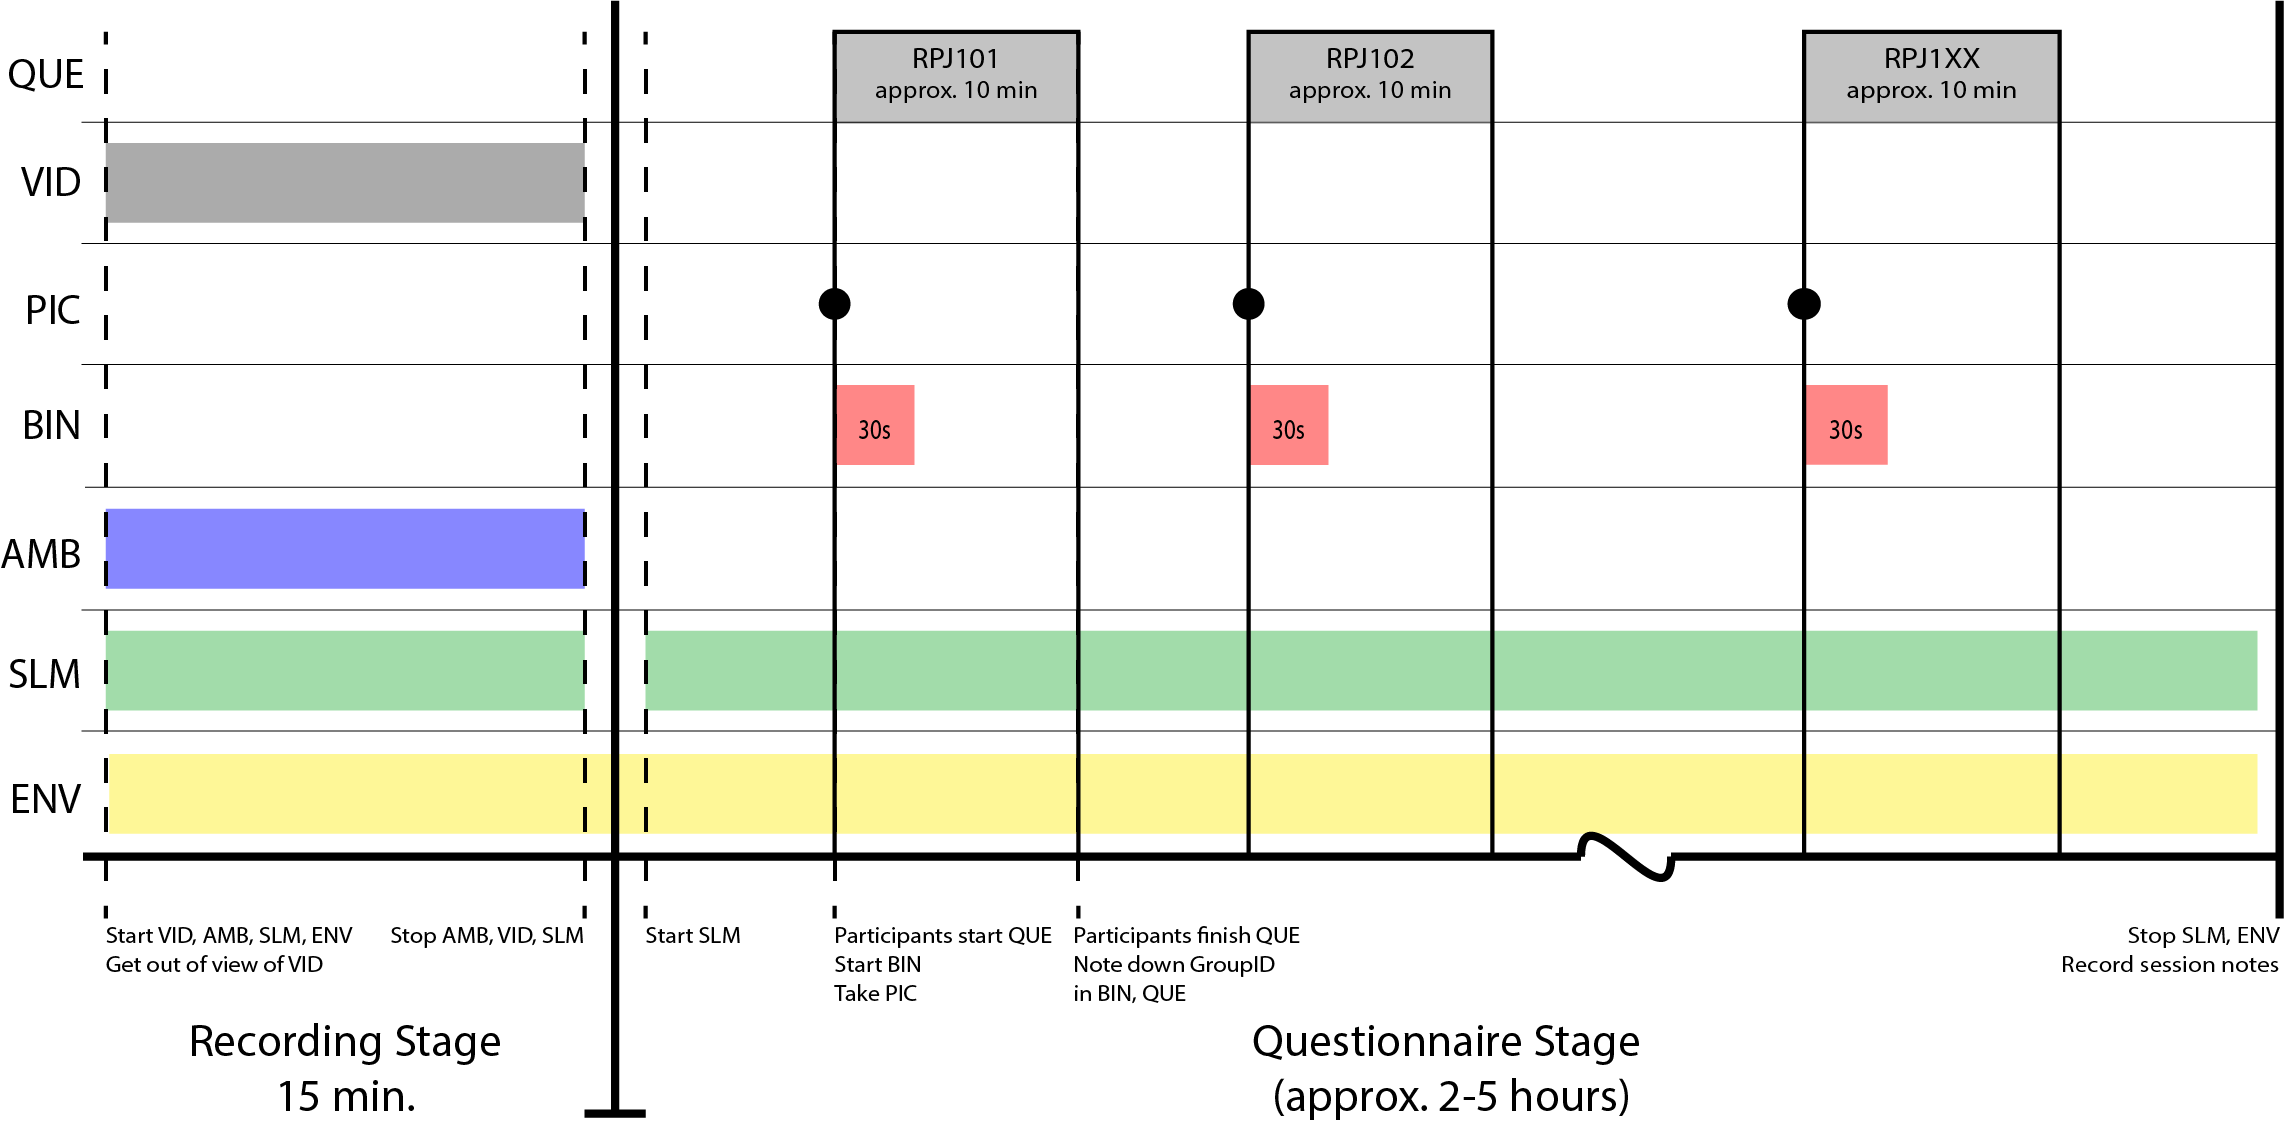
\includegraphics[width=\textwidth]{Figures/Survey-Diagram_V2}
   \caption{Timeline of the on site soundscape protocol. RegentsParkJapan (RPJ) is used as an example. Abbreviations as defined in Table \ref{tab:factors} -- \gls{que}: Questionnaires; \gls{vid}: 360\degree video; \gls{pic}: Site pictures; \gls{bin}: Binaural Recording; \gls{amb}: Ambisonic recording; \gls{slm}: Sound Level Meter (acoustical factors); \gls{env}: Environmental factors.}
   \label{fig:timeline}
 \end{figure}

 \paragraph*{Setup \& Calibration} The equipment should be assembled, checked, and calibrated prior to arriving at the measurement location. Calibrate the equipment according to the manufacturer's instructions. All \gls{slm}s should have built-in methods to calibrate using a standard 94 dB 1 kHz tone calibrator. If a similar method is available for the ambisonic microphone, this should be used. If a built-in method is not available, but a calibrator can be fitted to the microphone capsules, then the ambisonic microphone should be calibrated by recording the 1 kHz signal through the system for each microphone capsule after the gain settings have been finalised on site (see below). If it is not possible to calibrate the ambisonic microphone, then the levels recorded will need to be compared to the levels taken simultaneously with the \gls{slm}. This is why it is crucial to have an appropriate quality, calibrated \gls{slm} included within the same setup as the \gls{amb} recordings.

 \begin{figure}
   \centering
   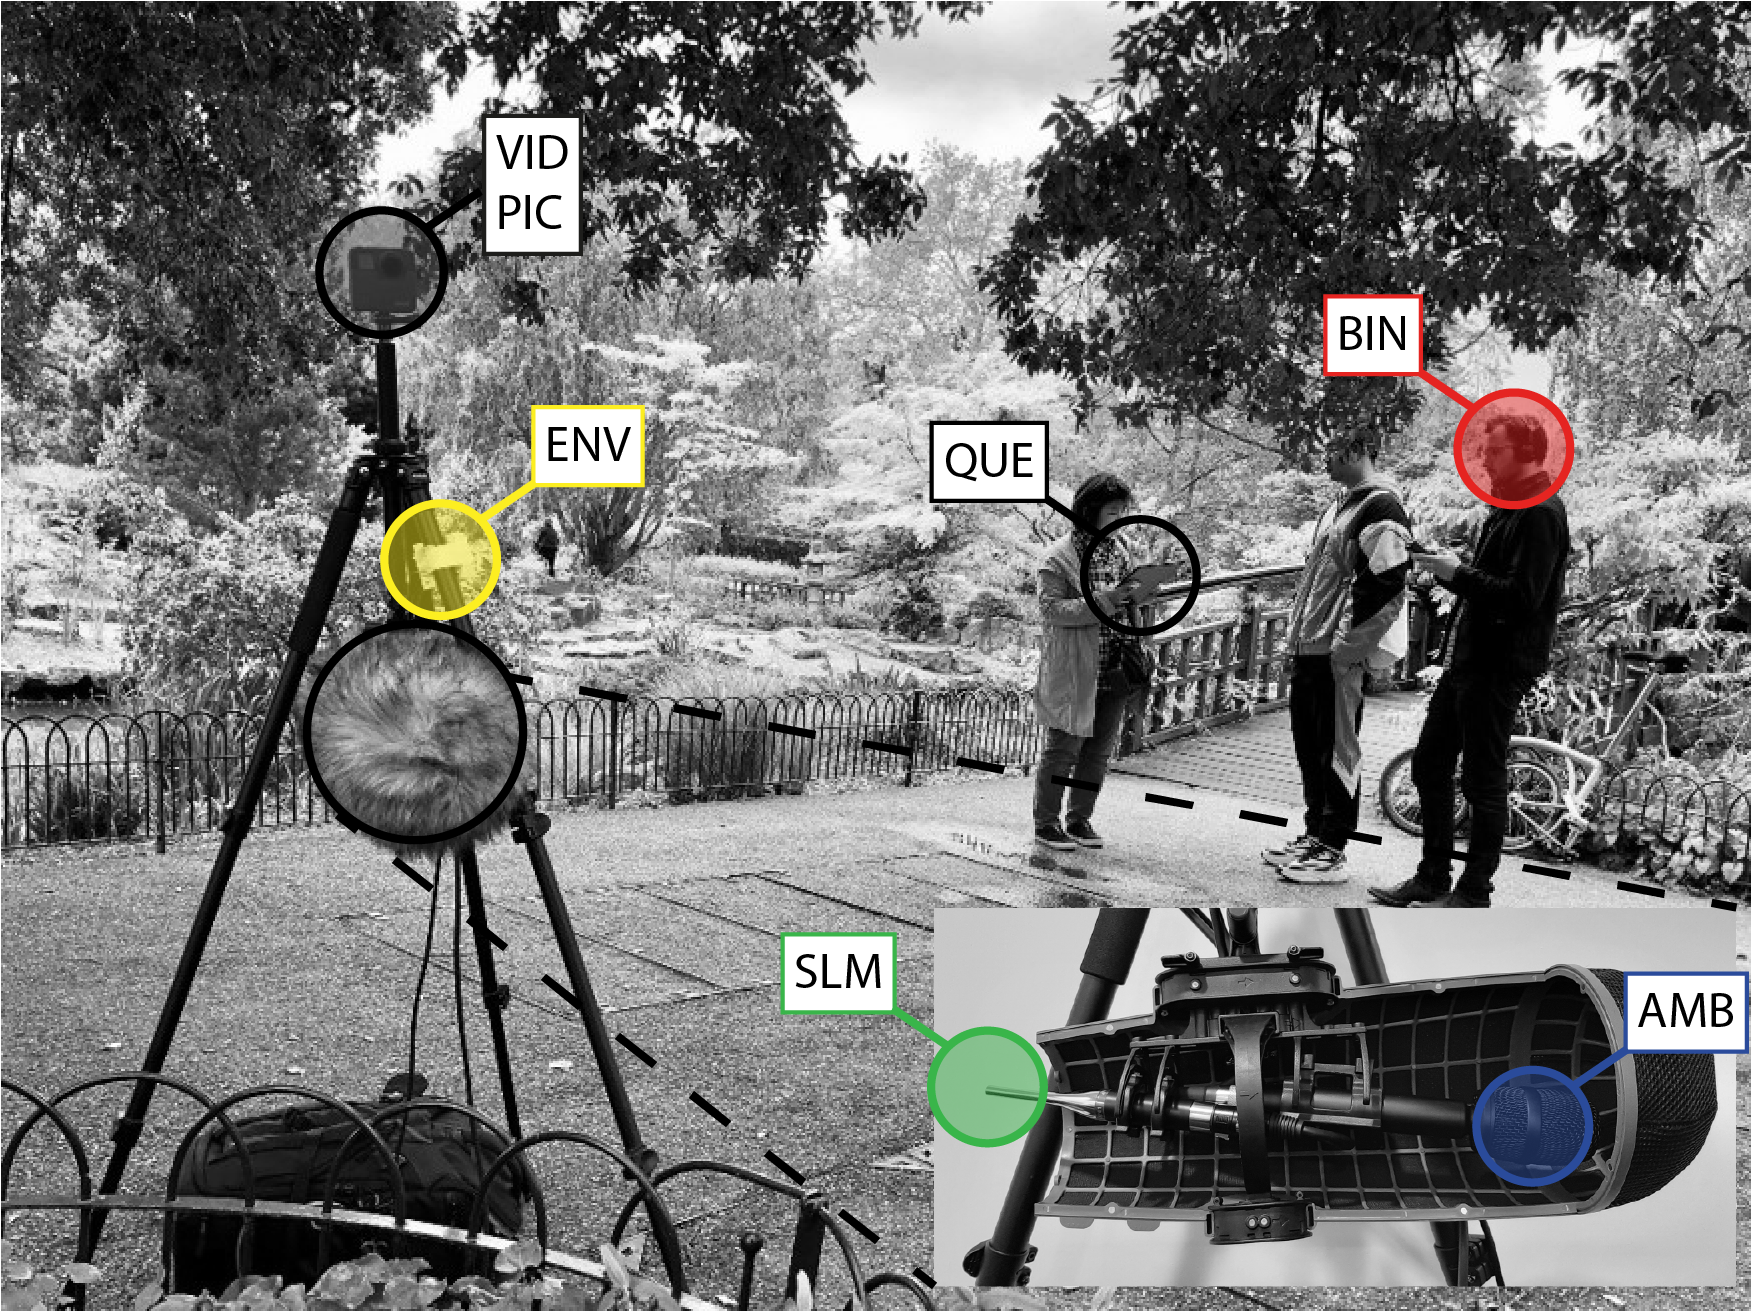
\includegraphics[width=\textwidth]{Figures/RegentsParkSurvey_V2-2}
   \caption{Photo of a full survey carried out in a park in London during the Questionnaire Stage. To the left is the equipment (colour-coded to match Figure \ref{fig:timeline}), with the ambisonic microphone and \gls{slm} microphone in the windscreen, with the 360\degree camera on top of the tripod and to the right are one researcher interacting with the participant while the second researcher conducts the binaural recording. The body of the \gls{slm} and the multi-channel recorder are stored in a bag under the tripod which can contain all of the pieces of equipment for easy transport.}
   \label{fig:survey-pic}
 \end{figure}

 \subsection{Assembling the Equipment}

   \begin{enumerate}
     \item Set up the equipment by prioritising the position of the 360\degree camera and position the lens at the average eye level 160--180 cm, as shown in Figure \ref{fig:survey-pic}.

           It is advisable to test the setup for video stitching issues and reconfigure if needed (e.g. the equipment will be partially visible in the raw video recording, so you need to test if the chosen setup allows for efficient erasing/hiding/patching of the exposed parts in the post-processing). Companies selling 360\degree cameras usually offer free software for basic editing and previewing. It is advisable to position the camera as the highest item in the set to avoid the need for editing both the sky and the ground.
     \item Carefully position the \gls{amb} microphone so its axes are aligned with the axes of the 360\degree camera; the microphone's front (usually marked by the logo) and the camera's front should be looking in the same direction. Many \gls{amb} microphones allow them to be oriented vertically or horizontally (end-fire), this should be noted and adjusted in the relevant software settings.

           This is essential for informed post-processing. It is advisable to position the capsules of the \gls{amb} microphone and the capsule of the \gls{slm} as near to each other as possible, without introducing scattering effects. It can usually be done within the same windshield unit, but it is not essential to do so and depends on the available clamps and stands.
     \item The gain settings for the four ambisonic audio channels should be set to the same level. In some devices (such as the MixPre10), this can be set by locking the channel gain settings to a single channel. Many devices also offer ambisonic plugins which simplify these settings and automatically link the gain settings -- these should be used where available.
     \item Set the \gls{slm} to log sound levels and simultaneously record .wav audio. The recommended logging settings are given in Table \ref{tab:equipment}. The \gls{slm} should be mounted and positioned according to standard guidance for environmental noise measurements, like that given in Section 9 of ISO 1996-2:2017 \cit{ISO1996} or Section 5 of ANSI/ASA S12.9-2013/Part 1 \cit{ANSI}. Generally, the microphone should be a minimum of 1.2m above the ground and a minimum of 1m from any vertical reflecting surfaces.
     \item Attach the environmental meter(s) to the tripod. Care should be taken when positioning the environmental monitor. Most units will include guidance on their use from the manufacturer -- these should be followed where available. Some general items to keep in mind include not accidentally covering air quality sensor holes, not positioning light sensors in the shade of the other equipment, and not positioning temperature sensors in direct sunlight unless this is how they are intended to be positioned.
   \end{enumerate}

 \subsection{Recording Stage}

   The following section prepares step-by-step instructions for conducting the Recording Stage of the on site protocol, as shown in Figure \ref{fig:timeline}.

   \begin{enumerate}
     \item Double check all settings and file save locations on the recording equipment.
     \item Adjust gain settings to ensure there is no clipping. Good practice is to listen for what is expected to be the loudest sound event during the recording period (e.g. sirens) and set the gain such that the level is comfortably under clipping during this event.
     \item Start recording on all devices, including the ambisonic microphone, 360\degree camera, \gls{slm}, and environmental meter.
     \item Stand at the front of the camera/ambisonic microphone and clap. The clap can help synchronise the audio with the video, if necessary, and ensuring you are standing in line with the front of the 360\degree video can help with lining up the directionality of the two, if necessary.
     \item Retreat out of view of the camera, blending into the surrounding crowd, or otherwise make sure not to be obvious to someone watching the video.
     \item Record at least 5 min of consistent and representative audio and video. It is recommended to record for 15 min to give the best chance of being able to extract a solid 5 min of useful video and audio.
     \item Stop recording on all devices and ensure all files are saved properly.
   \end{enumerate}

 \subsection{Questionnaire Stage}

   The following section prepares step-by-step instructions for conducting the in-situ questionnaires and their accompanying reference recordings as part of the Questionnaire Stage. Typically these are performed during the same working session as the Recording Stage, using the same set of equipment. The selection of an appropriate location and setup of the equipment should follow the guidance given in Section \ref{sec:location-selection}, while making sure the location selected is representative of where the respondents will be stopped. Wherever possible, the equipment should be assembled and located so as not to draw the attention of the respondents and particularly to avoid influencing their perception of the space.

   \begin{enumerate}
     \item Double check all settings and file save locations on the recording equipment. If starting this stage immediately after the Recording Stage, make sure to rename or advance the index of on the filenames for the \gls{slm} and \gls{env} meters.
     \item Start recording on the \gls{slm} and \gls{env} meter (or leave running from preceding Recording Stage). These will continue running until the end of the Questionnaire Stage.
     \item Gather the tablets and/or paper questionnaires and prepare to approach potential participants.
     \item Approach participants and ask if they would be willing to take part in a research study. If the participants are in a group, they can participate at the same time, but should each fill out a separate questionnaire. When approaching participants, you should identify yourself as a researcher or student researching urban sound. We %NOTE: May need to change pronouns here
           advise avoiding phrases such as "noise", "noise pollution", "noise disturbance" or other terms which carry a negative connotation. In general, explanations and answers to questions should strive to be as neutral as possible regarding the nature of the soundscape.
     \item Once the participant has consented to participate, hand them the questionnaire or tablet and provide them with basic instructions for answering the questionnaire. Emphasise that they should be responding and assessing the current sound environment, in the current place. Note that this is a common misunderstanding -- many participants assume the questionnaire is focussed on the sound environment at their home, or in the city in general. Where a mix of tablets and paper questionnaires are being used, each group should have at least one participant using a tablet such that start and end times and precise GPS coordinates can be pulled from the accompanying electronic questionnaire. While one researcher is interacting with the participants, the second should arrange the equipment for taking the \gls{bin} recordings and 360\degree photo (\gls{pic}).
     \item Once the participant has started answering the questionnaire, start recording the \gls{bin} audio. If the participants are in a group and all are taking the survey at the same time, only one binaural recording is needed for the whole group. The researcher conducting the recording should strive to keep their head as stationary as possible and to avoid making any extraneous noise.

           Make sure that at least 30s of consistent audio is recorded while the participant is filling in the questionnaire. This should not include talking either from the researcher or the participant. If talking or other intrusive (non-representative) sound occurs, extend the recording period to end up with a solid 30s of good audio. The goal is to capture the sound environment which the participant is exposed to while filling out their questionnaire, but to exclude sounds which the participant is not likely considering as part of their assessment. Most commonly, this would be the researcher talking, or the participant themselves talking. Any other sounds which the participant was "naturally" exposed to should be included.

           When taking the \gls{bin} recording, attempt to orient the head (artificial or researcher wearing a headset) in the same direction as the participants. This is not crucial as it is often impossible to achieve, but it is preferable. Be careful not to move the head during the recording.
     \item Note the GroupID in the metadata for the \gls{bin} recording, or make a manual note of the \gls{bin} recording file name and the GroupID separately.
     \item Take on 360\degree photo (\gls{pic}) with the camera to capture the general setting. This can also be done at regular intervals during the survey session.
     \item When the participant has finished filling in the questionnaire, thank them for their participation and fill in the additional research questions at the end of the questionnaire. These help to both track the data collected and to document the conditions on site. The most important of these are:
           \begin{itemize}
             \item (For paper version) Start and End time. If a Start time was not noted, at minimum, the End Time must be recorded and an average survey duration can be subtracted to estimate the Start Time.
             \item GroupID
             \item SessionID
           \end{itemize}
     \item Repeat steps 4--9 for the remainder of the session, incrementing the GroupID by one with each new group of participants. If there are more than two researchers on site, the additional researchers can stop new groups of participants simultaneously. The researcher operating the \gls{bin} equipment can then shift between the groups once they have finished the 30s recording. This researcher should also have the responsibility of keeping track of the GroupID numbers for each group. Experience has shown this is possible up to about three groups at a time, with four researchers on site.
     \item Once the session is finished, stop the equipment and ensure all files are saved properly.
     \item After each session, make note of the character of the site and the environmental conditions during the survey. This might include, but is not limited to:
           \begin{itemize}
             \item Site typology and intended use (e.g. urban park, transit station, urban square, etc.)
             \item Weather
             \item Crowdedness (i.e. how many people are present in the space)
             \item Dominant sound sources and any key soundmarks
             \item Visual character (e.g. amount of greenness, enclosed vs. open, etc.)
           \end{itemize}
   \end{enumerate}

\section{Lessons from International Data Collection}

 As this protocol has already been implemented by several research groups across four countries, it has undergone a rigorous testing and development process. Throughout this process, adjustments have been made which resulted in the final protocol presented here. However, no process is perfect or applicable in all situations. As such, after consultation with the research groups involved, we have compiled the most common feedback and guidance to keep in mind when implementing this protocol.

 \subsection{Sampling}

   The research groups were instructed to try keeping the structure of respondents well-balanced. This often led to longer times and larger sample sizes required as most comments from five research groups addressed age and type of location as the most influential factors for participant sampling. However, while some reported higher response rates from younger (student) members of the public, the others reported higher response rates in case of older highly-educated people. A common observation was that public parks are the locations with the highest response rates, most likely due to a high number of people taking part in activities that allow enough time to take part in a survey. The type of space was also reflected in the sense of privacy. In locations that were more public, people in groups were more likely to take part in the survey, while in the more private locations it was the opposite. Amongst other comments, whether a participant was a tourist or a local also had an influence on the response rate. Tourists seemed more likely to participate in the survey.

   Several groups reported excessive heat and cold to be negatively affecting the response rates. One research groups, which conducted the survey also in a residential area, distinguished privacy/ownership of the survey site as a major factor.

 \subsection{Data Collection}

   A group of three researchers seems to be the minimum number needed to conduct the survey, as observed by the partner research groups. A group of nine researchers on site proved to be the most effective number. The time needed to complete the survey varied greatly depending on the location.

   Although the questions are written in a manner that emphasises the focus on the actual acoustic environment perceived at the moment, additional care should be made to ensure a proper understanding of that concept while approaching the participants. Researchers' comments are invaluable here to keep track of the outliers if a researcher feels similar issues or other factors (i.e. wearing headphones) lead to collecting invalid or misleading data.

 \subsection{Equipment}

   Some partners had previous experience in soundscape research, but for all this was the first study that featured surveying a large number of public participants around a single measurement point. All the research groups found it very important to delegate one researcher or technician to care exclusively about the equipment and the quality of the recordings.

   The intention of the recording stage is to record a first-person experience most representative of the location. Therefore, the researchers are instructed to 'make themselves invisible' in the recording. However, at some locations, various research groups decided to put out a sign asking members of the public asking members of the public not to touch or come near the measurement point as they experienced passers-by touching the windshield out of curiosity.

   The equipment setup has been designed to be as compact and unobtrusive as possible so as to limit any intrusion on the participant's experience of the space. From our experience, most participants do not end up with the equipment within their field of view during the questionnaire and often do not notice the presence of the stationary equipment. In some locations, this is not possible and participants may comment on its presence; however, over the thousands of surveys collected, only a small number of respondents have commented on the equipment as noticeably impacting their experience.

 \subsection{Translation}

   Regarding the onsite soundscape survey, the translation of the questionnaires (and in particular the perceptual adjectives used for the soundscape appraisal) is a key point to consider when using the protocol in regions where English is not the local language. Indeed, while the ISO/TS 12913-2:2018 document from which the soundscape-related questions of this protocol are derived aims at providing standardised scales, it does not provide official translations in languages other than English. Some perceptual constructs are difficult to render in different languages and people might assign different meanings to them (e.g. \cit{51-54}). For this reason, in the soundscape research community, there is a growing interest in testing and validating reliable translation of the ISO soundscape adjectives \cit{Aletta SATP}, which will hopefully lead to a wide-spread use of this soundscape tool. It is expected that these validated translations could simply be substituted for their English counterparts in this protocol, when they become available.

\chapter{Psychological Well-being and Demographic Factors can Mediate Soundscape Pleasantness and Eventfulness}
\label{ch:whostudy}

\draft{This study will not be copied in wholesale. Instead, the goal is report the results in the context of working out the multi-level regression method and the influence of the non-acoustic factors. Would like to extend it by re-running the analysis with the full database, and controlling for binaural sound level.}

\section*{Context}

 Soundscape studies aim to consider the holistic human perception of a sound environment, including both the physical phenomena and how these are mediated by internal factors.

\section{Introduction}
\copied{From a physiological point of view, a sound signal is a detectable change in our external environment that can elicit a series of unconscious responses, unbalancing our homeostastis (the dynamic state of equilibrium). These responses are similar among populations in a similar situation, are automatic, and regulated by the \gls{sns}. The \gls{psns}, on the contrary, is constantly active to maintain homeostastis. It has long been established that both the \gls{sns} and \gls{psns} are part of the \gls{ans}, which is \emph{per se} a division of the \gls{pns} \cit{8}. Humans and soundscapes have a dynamic bidirectional relationship -- while humans and their behaviour directly influence their soundscape, humans and their behaviour are in turn influenced by their soundscape. Several scientific communities in the area of neuroscience and psychology, therefore, have begun to pay close attention to our day-to-day exposure to particular sounds and their impact on the mental and physical health of individuals. Researchers in the areas of acoustics, environmental psychology, and auditory neuroscience outline the adverse impact of noise or negative sounds on well-being in an attempt to improve modern living standards \cit{20-24}. In this regard, ,evidence indicates that positively perceived sounds (e.g. natural sounds) are tied with a high quality of life and enhanced physiological and physical health \cit{5, 25-27}. Subsequently, \gls{art} argues the impact of nature (e.g. being exposed to natural sounds such as waterfalls) on humans improved cognitive performance and stress recovery \cit{28-31}. Not only has spending time in nature been demonstrated to have positive effects on humans' nervous system but it has also been shown that humans innately tend to seek connections with nature, a hypothesis known as Biophilia \cit{32}. These theories and effects demonstrate the effect external environments have on the health and well-being of individuals, but this relationship is bidirectional within the mind as well. The prior mental and psychological state of the individual will also influence how that individual experiences the environment and can change their perception of it.}

\copied{The physiological and psychological approaches are two sides of the same coin in the realm of soundscape research, strongly interconnected and equally important. The psychological approach, in soundscape research, strives to depict the acoustic environment through the human behavioural pattern by borrowing a more deductive approach. It translates the underlying mechanisms into explicit behavioural manifestations, resulting from the perception of the acoustic environment. The physiological approach investigates the impact of the acoustic environment through the investigation of fundamental mechanisms of \gls{cns} and \gls{pns} by adopting a more inductive inferential approach. The physiological approach delineates the causation of the particular behaviour evoked by the environmental sounds.}

\copied{The soundscape is composed of three main components -- human interaction, acoustic environment, and perception -- so it potentially draws attention across several life-science disciplines such as environmental psychology and public health, psychophysiology, and auditory neuroscience. To the best of the author's knowledge, no work previous to this review has highlighted the explicit psychophysiological underpinnings of the soundscape. The review in this chapter is the first work that reflects the fundamental mechanisms of the soundscape rather than its behavioural expressions.}

\subsection{Psychophysiological studies}

\section[Methods]{Methods\footnote{This section closely resembles the original Methods section in \citep{Erfanian2021Psychological} of which I was the second author. I contributed significantly to the drafting of the original paper and the content presented here directly informs the analysis presented later.}}

The study was approved by the local ethics committee of University College London (UCL), BSEER, Institute for Environmental Design \& Engineering (IEDE) (Dated 11-10-2019).

\subsection{Data Collection}
This study made use of a subset of data from the \gls{isd}. This study was conducted and published during the first round of \gls{ssid} data collection, prior to the first publication of the ISD. It includes 11 locations in London, with data collected from general members of the public. This study made use of the same \gls{ssid} questionnaire presented in full in \cref{app:questionnaire}, which is an adapted version of \citet{ISO12913Part2}\footnote{The ISO/TS 12913-2:2018 specifies requirements and provides supporting information on data collection and reporting for soundscape studies, investigations, and applications.} Method `A' (urban soundwalk method) and the WHO-5 Well-being Index \citep{Hall2011Examining}, as well as demographic information. As this study focusses on the items related to psychological well-being, demographics, and personal factors, we used a subset of the variables available in the full ISD. Only the sections of the questionnaire which were examined within this study are reported in this chapter. \cref{tab:whoDemo} reports the demographic characteristics of the sample used.


\begin{table}[!ht]
  %TODO: Check the discrepancy in percentages between Employed and White - White has higher number but lower percentage?
\centering
\caption{The sample demographic characteristics \label{tab:whoDemo}}
% \resizebox{\textwidth}{!}{%
\begin{tabular}{@{}ll@{}}
\toprule
Demographic characteristics                 & N(\%)                            \\ \midrule
Total Samples                               & N = 1134                         \\
\textbf{Gender}                             &                                  \\
\quad Female                                & 610 (53.79)                      \\
\quad Male                                  & 524 (46.2)                       \\
\textbf{Age}                                &                                  \\
\quad Mean                                  & 34.67 years $\pm$ 15.11          \\
\quad 18-30                                 & 627 (55.29)                      \\
\quad 31-40                                 & 195 (17.19)                      \\
\quad 41-50                                 & 112 (9.87)                       \\
\quad 51-60                                 & 97  (8.55)                       \\
\quad 61-70                                 & 72  (6.34)                       \\
\quad 71+                                   & 31  (2.73)                       \\
\textbf{Educational Level}                  &                                  \\
\quad Some high school                      & 22  (1.2)                        \\
\quad High school graduate                  & 315 (17.3)                       \\
\quad Trade/technical/vocational training   & 51  (2.8)                        \\
\quad University (undergraduate/bachelor)   & 422 (32.1)                       \\
\quad Postgraduate degree (master)          & 324 (17.8)                       \\
\textbf{Occupation Status}                  &                                  \\
\quad Employed                              & 613 (54.05)                      \\ 
\quad Unemployed                            & 25  (2.2)                        \\
\quad Retired                               & 84  (7.4)                        \\
\quad Student                               & 348 (30.6)                       \\
\quad Employed-Student                      & 5   (0.4)                        \\
\quad Other                                 & 44  (3.8)                        \\
\quad Rather not say                        & 15  (1.3)                        \\
\textbf{Ethnicity}                          &                                  \\
\quad White                                 & 806 (71.08)                      \\
\quad Mixed/Multiple ethnic groups          & 63  (3.5)                        \\
\quad Asian/Asian British                   & 156 (8.6)                        \\
\quad Black/African/Caribbean/Black British & 31  (1.7)                        \\
\quad Middle Eastern                        & 23  (1.3)                        \\
\quad Rather not say                        & 55  (3)                          \\
\bottomrule
\end{tabular}%
% }
\end{table}

\subsubsection*{Perceived affective quality / Perceptual attributes}

\copied{The \glsfirst{paq} of the sound environment as adopted in Method `A', described in \citet{ISO12913Part2}, consists of category scales containing five response categories, based on the \gls{ssqp} \cite{Axelsson2012Swedish}. It includes a question `to what extent they agree/disagree that the present surrounding sound environment is \ldots'. The participants judged the quality of the acoustic environment by 8 adjectives: pleasant, chaotic, vibrant, uneventful, calm, annoying, eventful, or monotonous. The answers were presented in a 5-point Likert scale ranging from `strongly disagree = 1' to `strongly agree = 5'. The perceptual attributes measure as a unidimensional measuring tool for the perception of the acoustic environment has not been validated to this date. The \glspl{paq} were utilised as aggregated values to construct the principal components of the soundscape (\gls{isopl} and \gls{isoev}) (see \cref{sec:whoOutcomeVar}).}

In order to maintain data quality and exclude cases where respondents either clearly did not understand the \gls{paq} adjectives or intentionally misrepresented their answers, surveys for which the same response was given for every \gls{paq} (e.g. `Strongly agree' to all 8 attributes) were excluded. This is justified as no reasonable respondent who understood the questions would answer that they `strongly agree' that a soundscape is pleasant and annoying, calm and chaotic, etc. Cases where respondents answered `Neutral' to all \glspl{paq} are not excluded in this way, as a neutral response to all attributes is not necessarily contradictory. In addition, surveys were discarded as incomplete if more than 50\% of the \gls{paq} and sound source questions were not completed. 

\subsubsection*{Psychological well-being/WHO-5 well-being index}

\copied{The \glsfirst{who5} asks how individuals have been feeling over the last two weeks such as `I have felt cheerful and in good spirits'. The \gls{who5} has been designed for multiple research and clinical purposes, covering a wide range of mental health domains, namely perinatal mental health, geriatrics mental health, endocrinology, clinical psychometrics, and psychiatric disorders screening.}

\copied{The \gls{who5} is known to be one of the most valid generic scales for quantification of general well-being. In terms of the construct validity of the scale, \gls{who5} shoed to have properties that are a coherent measure of well-being \citep{Topp2015WHO}. With regards to relevant literature, \gls{who5} confirmed that all items constitute an integrated scale in which items add up related information about the level of general pscyhological well-being among both youngsters and elderlies \cit{Blom2012, Lucas-Carrasco2012}. For the purpose of analysis, a composite \gls{who5} score is calculated by summing the responses to each of the 5 questions (coded from 0 (for `at no time') to 5 (for `all of the time')), then multiplying by 4 to get a single score which ranges from 0 (the lowest level of well-being) to 100 ( the highest level of well-being) \citep{Topp2015WHO}.}

\subsubsection*{Demographic characteristics}

\copied{Demographic characteristics were presented such as age, gender (male, female), education level (some high school, high school, trade/technical/vocational training, university, and postgraduate), occupational status (employed, unemployed, retired, student, employed-student, other, and rather not say), and ethnicity (Asian, Black/Caribbean, Middle Eastern, White, and Mixed). Some blank spaces were provided if the participant wished to add further information. At the end of the survey, participants had the opportunity to write down any additional questions or remarks and were thanked for their participation.}

\subsubsection*{Outcome variables (\gls{isopl} and \gls{isoev})}

The soundscape data were analysed according to the procedure laid out in Part 3 of the ISO 12913 \footnote{The ISO/TS 12913-3:2019 provides requirements and supporting information on analysis of data collected \emph{in-situ}.} standard series. In order to ease data analysis and modelling, the standard suggests a method to collapse the \gls{paq} responses for each of the 8 \glspl{pa} down to a 2-dimensional coordinate scatter plot with continuous values for `Pleasantness' on the X-axis (referred to as \gls{isopl}) and `Eventfulness' on the Y-axis (referred to as \gls{isoev}). These coordinates are then normalized to between -1 and 1 (per the recommendation of \citet{ISO12913Part3}).

\subsubsection*{Survey procedure}

The data was collected according to the \gls{ssid} protocol outlined in \cref{chap:protocol}. The goal of the researchers on site was to collect a minimum of one hundred questionnaires from each selected site/location, which was typically achieved over a period of 2-3 days each consisting of approximately a 4 hour session. In some cases, either due to extenuating circumstances, time constraints, or excluded surveys, the full one hundred surveys were not achieved. The data for this study were collected from \nth{28} February 2019 to \nth{18} October 2019 between 11 a.m. and 3 p.m.

In line with the \gls{ssid} protocol, during the survey period, acoustic and environmental metrics were simultaneously collected through binaural recordings, a calibrated \gls{slm}, and an environmental meter which recorded temperature, lighting level, and humidity data. The \gls{slm} was set up in the space in which the questionnaires were conducted (i.e. the \gls{environmental-unit}) and left running for the full duration of the survey in order to characterise the acoustic environment. The environmental metrics were not reported in this study since they were not in the scope of this paper but are included in \cref{app:location-data} in order to provide context for the interested readers. 

\subsection{Data analysis strategy}

\subsubsection*{Missing data, checking for outliers, and data scaling}

Prior to the data analysis, I imputed missing data and the imputed data was used across all analyses. Missing education values were imputed with the mode value (University). Missing values for age were imputed with the median age value (29). \gls{who5} (psychological well-being) missing values were imputed with the median value (64). I excluded those who responded `non-conforming' (N=4) or `decline' (N=21) for gender, due to the very small sample size and to simplify the effects of gender in the model. The initial data sample size was N=1467; the data included in the analysis N=1134.

I took a lenient approach to outliers. Due to the nature of survey data, it was typically inappropriate to remove data solely because it represented a deviation from the typical response. However, I wanted to catch data which was incorrect, intentionally wrong, or a typo and then remove them. For the most part, this was handled with our data quality method implemented in REDCap, to ensure the \gls{ssqp}/perceptual attribute values (N=8) were filled in such that they complied with the circumplex theory to a minimum degree. We were therefore, only looking for values which were extreme outliers or impossible.

\subsubsection*{Correlation between predictors and output variables}
To establish the linearity between all pairs of variables including the predictors and outcome variables, the Pearson correlation coefficient, \gls{anova}, and Chi-square were performed between psychological well-being, age, gender, ethnicity, education level, occupation status, and the circumplex coordinate values (\gls{isopl} and \gls{isoev}). These results are given in \cref{tab:whoCorr}.

\subsection{Model specification (linear mixed-effects modelling)}

\glsfirst{lmer} with random intercept and fixed slope, using backward stepwise feature selection was utilised to (a) identify the association of our features of interest (FOIs) including psychological well-being, age, gender, education level, ethnicity, occupation status, and their interaction terms with \gls{isopl} and \gls{isoev} and (b) accommodate associations within participants among locations. In order to account for latent differences in the pleasantness and eventfulness ratings of various locations, the intercepts of each model are allowed to vary as a function of the location. Therefore, the model is constructed with two levels -- the individual level (the random effects) and the location level (the fixed effects). Separate models were constructed for each \gls{isopl} and \gls{isoev} and take the form:
%
\begin{equation}
  \label{eqn:whoPl}
  ISOPleasant_{ij} = \beta_{0j} + \beta_1 x_{1ij} + \beta_2 x_{2ij} + \ldots + \beta_n x_{nij} + \epsilon_{ij}
\end{equation}
%
\begin{equation}
  \label{eqn:whoEv}
  ISOEventful_{ij} = \beta_{0j} + \beta_1 x_{1ij} + \beta_2 x_{2ij} + \ldots + \beta_n x_{nij} + \epsilon_{ij}
\end{equation}
%
where $ISOPleasant_{ij}$ or $ISOEventful_{ij}$ are the dependent variable value for individual $i$ in Location $j$; $\beta_{0j}$ is the intercept for Location $j$; $\beta_1$ through $\beta_n$ are the slopes relating the independent variables $x_1$ through $x_n$ to the dependent variable; $x_{1ij}$ through $x_{nij}$ are the dependent variables for individual $i$ in Location $j$; $\epsilon_{ij}$ is the random error for individual $i$ in Location $j$. In turn, $\beta_{0j}$ can be expressed as:
%
\begin{equation}
  \beta_{0j} = \gamma_{00} + U_{0j}
\end{equation}
%
where $\gamma_{00}$ is the mean intercept across Locations; and $U_{0j}$ is the unique effect of Location $j$ on the intercept. In a random intercept model, the slope coefficients ($B_n$) are considered fixed across the locations (hence, labelled as the fixed effects) indicating that the relationship between the dependent variable (e.g. age, gender, etc.) and the independent variable (\gls{isopl} or \gls{isoev}) is the same for all locations, while the general \gls{isopl} of the location is accounted for by the varying intercept.

In order to identify the significant FOIs within the multi-level structure, we employed a stepwise feature selection on the fixed effects portion of the mixed-effects model, with an inclusion threshold of $p < 0.05$. Since this model includes only the LocationID at the random effects level, only the fixed effects are reduced in the feature selection process. To check for multicollinearity among the selected features, the \glsfirst{vif} was calculated and a threshold of $VIF < 5$ was set. Any features which remained after the backwards stepwise selection which exceeded this threshold were investigated and removed if they were highly collinear with the other features. Once the feature selection process is completed, the final model with only significant FOIs included is fit and the table of the model coefficients is printed along with plots of the random effects and z-scaled and non-standardised estimates terms. 

The model fitting and feature selection was performed using `lme4' (version 1.1) and the `step' function from `lmerTest' (version 3.1.3) \cit{Kuznetsova, Brokhoff, Christensen, 2017} in R statistical software (version 4.0.3) \cit{R core team, 2013}. The summaries and plots were created using the `sjPlot' package (version 2.8.6) \cit{Ludecke, 2018}. 

\section{Results}

The setup and procedures %TODO: Return here

\section{Discussion}
 \subsection{Incorporating personal factors into a predictive soundscape model}
Although, as \citet{Droumeva2021sound} points out, each individual brings their own cultural and subjective aspects of listening to the stage of urban sound, when attempting to characterise the soundscape of a space, it is not a particular individual's aspects we should be concerned with. That individual forms a part of the collective perception of the space. Their cultural and subjective (i.e. personal) aspects mitigate their perception, but this perception then forms only a single component of the collective perception. How then should we consider these personal factors? Surely there is no suggestion to disregard their influence and importance within the soundscape approach? In my view, there are two approaches:

\begin{enumerate}
  \item Incorporate these personal factors as demographic statistics of a location; or
  \item An agent-based approach where each individual likely to use the space is simulated and modelled with their personal factors to then be included in the collective perception.
\end{enumerate}

Let's look at how these two approaches would be implemented in a multilevel acoustics-based predictive model, such as those presented in \crefrange{ch:mlmann}{ch:lockdown}.

\subsubsection{Approach 1}
In the first, the demographic breakdown of the space under investigation is estimated, either through a census or by the designers' desired use case. This demographic breakdown can then be compared to the results presented above \citep{Erfanian2021Psychological} to derive weighting factors which adjust the predicted soundscape assessment. For instance, the results suggest that retired persons perceive the soundscape as \draft{XX\% or amount [need to check with results]} less pleasant than others. If the particular space under investigation has a large proportion of retired persons, say 65\% we could then apply an adjustment to the initial personal-factors-agnostic prediction to reflect this tendency. In this example, an initial location-level \gls{isopl} prediction of 0.36, with a 65\% retired population would be corrected by \draft{-XX [0.65 x result]} for a final demographics-corrected \gls{isopl} prediction of \draft{XX}.

\subsubsection{Approach 2}

\subsubsection{Benefits and downsides of each approach}

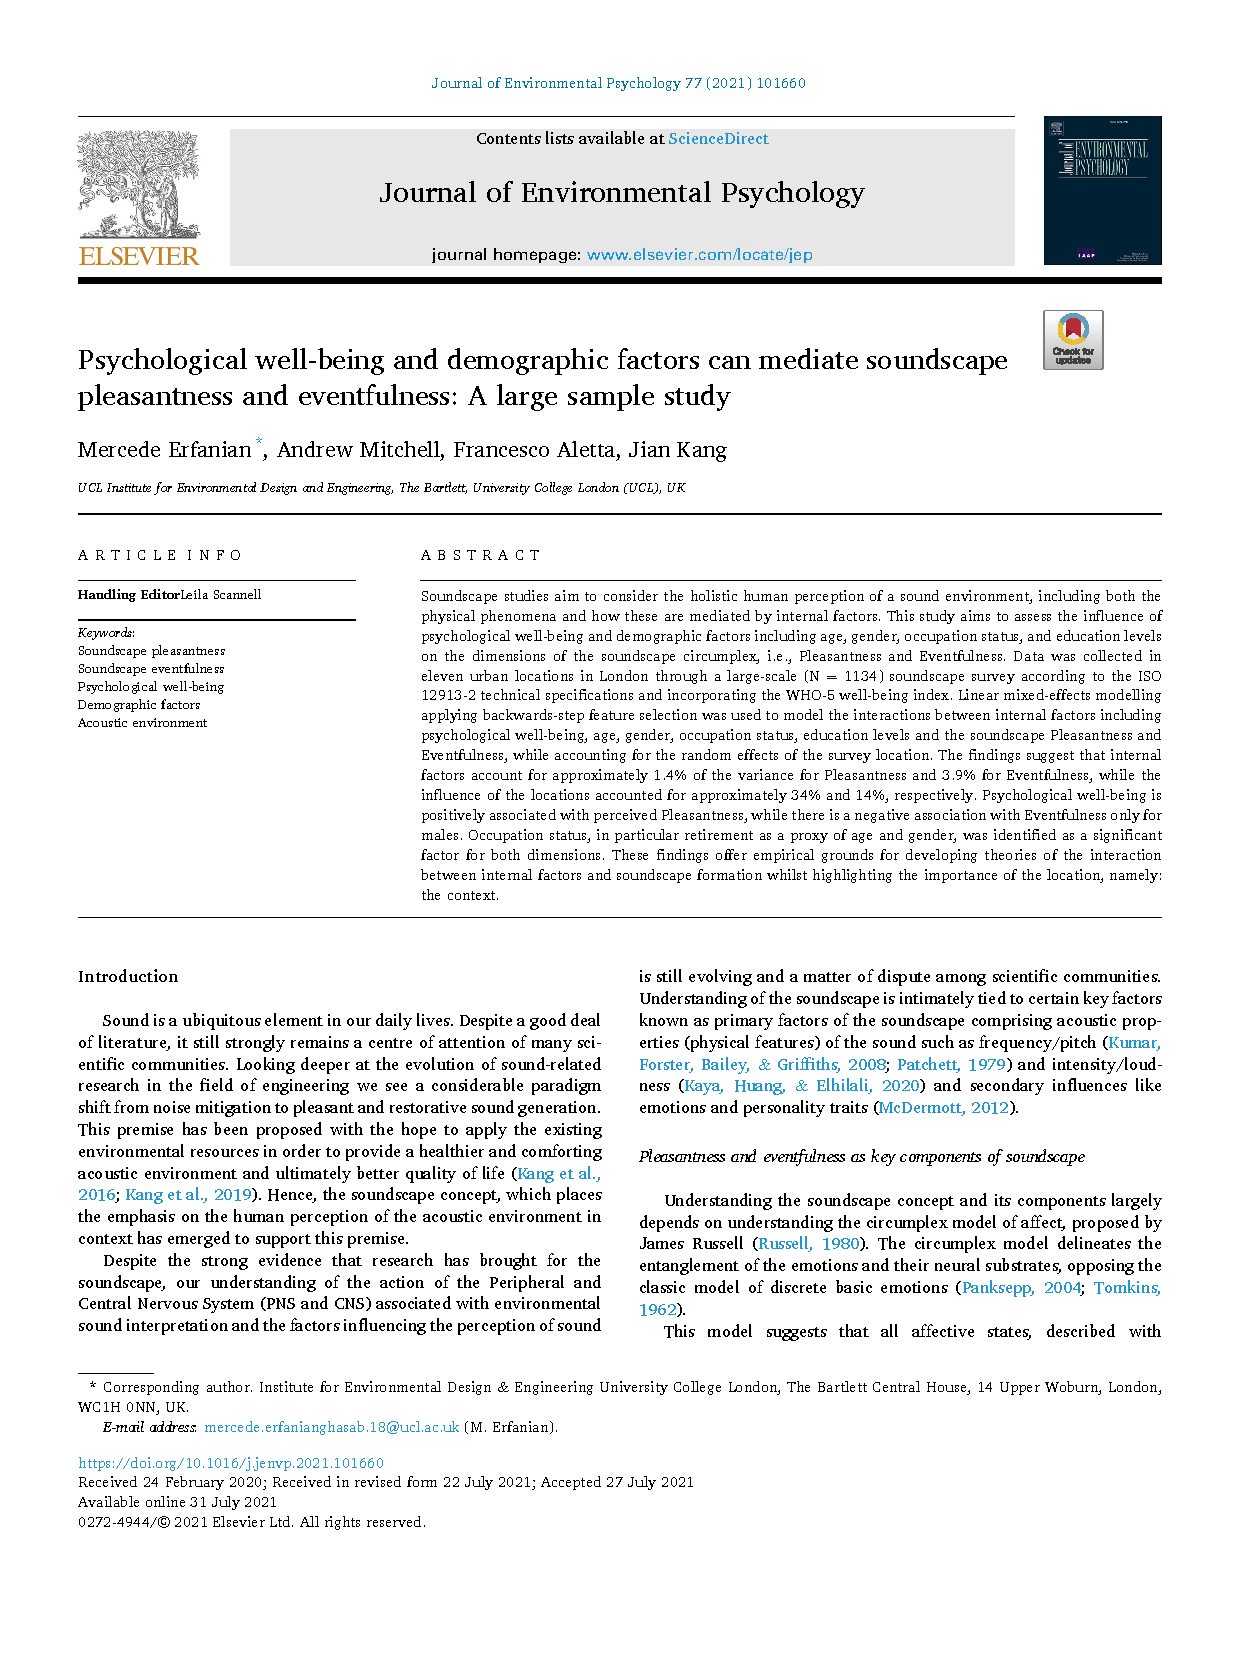
\includepdf[pages={1-8}]{./Papers/Erfanian2021Psychological - Psychological Well Being and Demographic Factors Can Mediate Soundscape Pleasantness and Eventfulness_ a Large Sample Study.pdf}

\chapter{Multilevel Annoyance Modelling of Short Environmental Sound Recordings Including Sound Source Information}
\label{ch:mlmann}

\section*{Context}
Published as: Orga, F., \textbf{Mitchell, A.}\footnote{Joint first author}, Freixes, M., Aletta, F., Alsina-Pagès, R. M., \& Foraster, M. (2021). Multilevel Annoyance Modelling of Short Environmental Sound Recordings. \emph{Sustainability, 13}(11), Article 11. \url{https://doi.org/10.3390/su13115779}

%TODO: Need to heavily edit this to rephrase and to re focus on my work
\draft{This chapter will be re-worded and somewhat reorganised to better fit my thinking and to highlight the analysis work. Its focus within the thesis is on the use of sound source information to improve the prediction of annoyance. Right now this is wholesale copied from the published paper.}

\section*{Abstract}

 \draft{The recent development and deployment of Wireless Acoustic Sensor Networks (WASN) present new ways to address urban acoustic challenges in a smart city context. A focus on improving quality of life forms the core of smart-city design paradigms and cannot be limited to simply measuring objective environmental factors, but should also consider the perceptual, psychological, and health impacts on citizens. This study therefore makes use of short (1 - 2.7s) recordings sourced from a WASN in Milan which were grouped into various environmental sound source types and given an annoyance rating via an online survey with $N=100$ participants. A multilevel psychoacoustic model was found to achieve an overall $R^2=0.64$ which incorporates Sharpness as a fixed effect regardless of the sound source type and Roughness, Impulsiveness, and Tonality as random effects whose coefficients vary depending on the sound source. These results present a promising step torward implementing an on-sensor annoyance model which incorporates psychoacoustic features and sound source type, and is ultimately not dependent on sound level.}

\section{Introduction}

 \draft{Noise has been proven to have a wide impact on the social and economic aspects of citizens' lives \citep{Goines2007Noise} and is regarded as one of the primary environmental health issues referenced in the new environmental noise guidelines \citep{Nations2018World}. Over the past few years, several research teams have analysed the causes and the impact of this noise, revealling that it causes more than 48,000 new cases of ischemic heart disease and around 12,000 deaths in Europe each year \citep{Blanes2017Noise}. Furthermore, it leads to chronic high annoyance for more than 22 million people, and sleep disturbance for more than 6.5 million people \citep{Ndrepepa2011Relationship}. One of the main noise sources according to research is road traffic noise \citep{Ouis2001Annoyance}, causing psychological reactions in citizens \citet{Basner2006Aircraft} and even cardiovascular diseases \citep{Ndrepepa2011Relationship}.}

 \draft{Other studies analyse the effects of aircraft noise on sleep \cit{} and learning impairments in children \cit{}. Also, railway noise has proven to cause annoyance due to its huge variety of sounds, e.g. rail breaks, whistles, squeals, and vibrations \cit{ 8, 9}. Most of the literature focuses on sound level measurements and the corresponding annoyance \cit{ 10}, but other acoustical and psychoacoustical characteristics could be taken into account, e.g. loudness or sharpness \cit{ 11}, in order to understand the degree of noise annoyance and identify the characteristics of sounds that may be more detrimental to psychological well-being and consequently for health. Such knowledge is relevant for policy makers and urban planners in order to create healthy environments.}

 \draft{Several tests used in studies to evaluate the effects of environmental noise for citizens \cit{ 12} can be used to design this model. This study uses real-life data and its sound characterisation, thus focusing on noise sensitivity was not the closes approach to the problem. The tests used as a basis in this work have been defined with the purpose of finding new ways of analysing the impact of sound -- usually traffic -- on citizens in urban environments \cit{ 13, 14}, in order to model the annoyance perception \cit{15, 16}.}

 \draft{The perceptual tests were designed to measure the annoyance in people relating to different urban sounds and their characteristics \cit{ 17, 18}, by means of short excerpts of raw acoustic audio obtained from the DYNAMAP project \cit{ 19}. The most representative audio excerpts were selected, using a wide range of sound types (sirens, airplanes, people talking, dogs barking, etc.) \cit{ 20, 21}. However, sound annoyance depends on the acoustic characterisation of each sample, and it is possible to classify the acoustic excerpts depending on their characterisation, which can be the basis to ask participants about their perceptions. The characterisation is based on the psychoacoustic measurements of loudness, sharpness, and others defined by Zwicker \cit{ 11}.}

 % FIXME will need to rewrite this paragraph, not happy with it.
 \draft{The researchers asked more than 100 people to conduct the perceptual tests \cit{18}. Some preliminary results of the three tests conducted were published in \cit{17} in which the relationship between sharpness and annoyance was analysed by means of an A/B test \cit{22}, and later on in \cit{18}, where some of the research questions were formulated. In this study, I aim to determine the parameters that have an effect in the individual annoyance scores. For this reason, a multilevel psychoacoustic model is trained using the results of the MUSHRA \cit{23} test, essentially focused on annoyance evaluation by the participants over several different types of sound, while loudness and sharpness were kept constant. The results show that the differences in annoyance perception between the different demographic groups is not statistically significant and that sharpness is the main predictor for annoyance.}

 The chapter is structured as follows: Section \ref{sec:mod} detailes the state-of-the-art of annoyance modelling by means of subjective data collection. Section \ref{sec:proc} describes the procedure followed in this work, including the dataset and the design of the perceptual test. In section \ref{sec:res} the results obtained from the perception tests are presented and discussed, and the annoyance model is proposed. Section \ref{sec:disc} contains the discussion and, finally, Section \ref{sec:conc} presents the conclusions of the study.

\section{State of the Art of Annoyance Evaluation and Modelling}
 \label{sec:mod}
 In this section I gather a short synthesis of the most relevant contributions of the state-of-the-art on which the design of the tests and the modelling of perceptual annoyance have been based.

 \subsection{Evaluation of Annoyance}
   % FIXME prob need to rewrite this
   \draft{The evaluation of annoyance can be found in literature by means of the objective parameters related to sound and noise \cit{10}. Nevertheless, when the goal is to measure the perception -- the real annoyance experienced by people -- one of the most frequently used methods is to conduct a survey to measure the degree of annoyance produced by different sounds \cit{24, 25,26}. Following the recommendation of the International Committee for the Biological Effects of Noise (ICBEN), this evaluation should be done in a qualitative way, using a verbal scale; this can be translated into \emph{not at all, slightly, moderately, very} and \emph{extremely}, just to give a few examples. Also an 11-point scale -- also from an ICBEN recommendation -- can be used, where in this case, zero corresponds to \emph{not at all} and 10 corresponds to \emph{extremely disturbing}.}

   % FIXME take this paragraph out
   \draft{Furthermore, taking advantage of the experience in soundscape evaluation \cit{27} citizens can be asked about other aspects besides annoyance. To this end a perceptual assessment based on a Likert scale \cit{28} could be used. This scale defines five levels of agreement with a given statement: \emph{Strongly disagree, Disagree, Neither agree nor disagree, Agree} and \emph{Strongly agree}. This scale was used in \cit{17,18} to evaluate several types of noise sources according to a small group of attributes such as \emph{loud, shrill, noisy, disturbing, sharp, exciting, calming} and \emph{pleasant} (see the complete list of adjectives in \cit{27}).}

  Borrowing from the subjective assessment of audio quality, the MUSHRA method has been also used for the evaluation of annoyance in \cit{17, 18}. \gls{mushra} was described and designed by ITU-R under the recommendation ITU-R BS.1534-3 \cit{23}. This recommendation gives guidelines on listening tests and subjective assessment, as well as audio quality (among other applications), assuming that the best way to evaluate audio quality is by means of subjective listening.

   Listening tests can be conducted in a controlled scenario (e.g. in an anechoic chamber) thus allowing the organiser to have control over the setup and experimental design. Nevertheless, this approach is expensive and time consuming. Alternatively, online listening tests have been widely used in the perceptual evaluation of audio quality or speech synthesis systems, even resorting to crowdsourcing strategies \cit{29}. These tests can be run in parallel and anywhere, thereby reducing costs and allowing researchers to reach a wider audience \cit{30}. In addition, these tests have seen increased use in the wake of the \gls{covid19} pandemic and its subsequent lockdowns. The limited access to facilities and equipment restricted how socio-acoustic and laboratory studies could be conducted, leading to the development of new online data collection methods. Recommendations for conducting such studies were given by \draft{the Acoustical Society of America in \cit{that guidance site}}. %TODO: Expand on this bit?

 \subsection{Annoyance Prediction}
   \draft{After the design and execution of the perceptual tests, the resulting evaluation coming from participants are used to generate a model that can predict the annoyance value depending on the type and the parameters of the noise excerpt under study. One of the most representative examples of annoyance modelling is found in \cit{15}, where a model based on the hypothesis that annoyance is primarily determined by the detection of intruding sounds is presented. The model takes into account several measurable elements:}

   \begin{enumerate}
     \item signal-to-noise ratio (SNR);
     \item indoor background level;
     \item the activity conducted by the listener, assuming that in the conducted tests, their main activity is not listening to events.
   \end{enumerate}

   \draft{The model is obtained from the results of a test evaluating annoyance and acoustic data from a field experiment in a natural setting.}

   Another reference model for annoyance prediction is found in \cit{16}, where the authors model and predict road traffic noise annoyance based on:
   \begin{enumerate}
     \item noise perception;
     \item noise exposure levels;
     \item demographics.
   \end{enumerate}

   \draft{The authors apply machine-learning algorithms in order to conduct the prediction and measure error rates, which give them a good trade-off in the prediction of the traffic noise annoyance, with a strong dependence on subjective noise perception and predicted noise exposure levels, assuming that the classical statistical approaches fail in their predictions in terms of accuracy.} % REVIEW should/could rewrite this last bit

   A model of annoyance based on a combination of psychoacoustic metrics was proposed by \citet{PsychoacousticsfactsmodelsZwicker}. Generated from laboratory-collected data, this model attempts to provide a method to directly calculate the relative annoyance values of single-source sounds from the psychoacoustic Loudness, Roughness, Sharpness, and Fluctuation Strength. this model has also been further expanded upon to include a term for the Tonality of the sound \cit{31}. However, this model was developed based on laboratory studies of generated, simple sounds (i.e. not real recorded sounds) and does not take into account the semantic information associated with the real environmental sounds present in an urban environment.

   In \cit{32}, the authors led us to a better understanding of the transportation noise-annoyance response, in three different and relevant approximations:

   \begin{enumerate}
     \item to unravel the factors that affect the annoyance response of people in reference to the mixed transportation noise;
     \item to contrast the noise-annoyance dependence in situations where road traffic and railway noise dominate;
     \item to detail the differences between those two using structural equation modelling.
   \end{enumerate}

   As expected, the results show that annoyance is largely determined by noise disturbance and the noisiness perceived by citizens. Finally, in \cit{33} an approach to develop a road traffic noise prediction model is presented, and it takes into account:

   \begin{enumerate}
     \item social aspects
     \item characteristics of traffic, and
     \item urban development
   \end{enumerate}

   It is based on the creation of a local model, with a pilot in Istanbul (Turkey), which uses all the information gathered for the creation of the noise maps as an input, and provides annoyance levels prediction as an output, complementing the noise maps which provide no subjective indicator.

\section{Methods}

 In this section, I detail the several methods applied in this experiment from the perceptual test design based on an urban sound dataset \cit{21} to the multilevel linear regression modelling applied to obtain the annoyance prediction.

 \subsection{Dataset}
   %TODO: Read LIFE DYNAMAP papers and summarise dataset collection. 
   This study makes use of a dataset collected in collaboration with the LIFE DYNAMAP project conducted in Milan (Italy) \cit{19, 21}. This project makes use of a \gls{wasn}, enabling the collection of a large quantity of data over a longer period of time than was possible with the \gls{ssid} protocol outlined in \cref{chap:protocol}. 
  %  In order to obtain a proper representation of the acoustic environment in the design of the perceptual tests, a large quantity of recorded data is needed. The data gathered in this project belongs to different recording times and urban locations, using the \gls{wasn} deployed in Milan (Italy) in the framework of the LIFE DYNAMAP project \cit{19, 21}
A \gls{wasn} enables a broader characterisation of the acoustic events present in a location, as recording conditions can be made consistent across the nodes and data can be retrieved at any time of the day.
  %  Gathering the data through a \gls{wasn} facilitates the collection of a wide and accurate representation of the acoustic events, because it keeps the same recording conditions in every node and allows the retrieval of data at any time of the day. 
   \draft{The dataset used in this study has been obtained by homogeneously sampling several hours, in both weekday and weekend, with 24 sensors distributed along the urban District 9 of Milan \cit{34}. After that, experts from the DYNAMAP development team labelled the acoustic events of the recordings manually to obtain a 151-h dataset \cit{21}. Due to the nature of the project, that consisted in removing events not related to traffic noise from the noise map computation, events were grouped in \gls{rtn} that belongs to the 83.7\% of the total time of the dataset, and \gls{ane} with the 8.7\% of the total time. Another class was used to include overlapping and unidentified events: \gls{complx} with 7.6\% of the total time \cit{20}. During the labelling process, the DYNAMAP developers found up to 26 types of anomalous events, which they decided to group in the following classes: airplane, alarm, bell, bike, bird, blind, brake, bus door, construction, dog, door, glass, horn, interference, music, people, rain, rubbish service, siren, squeak, step, thunder, tramway, train, trolley, wind, works (construction) \cit{35}.}

   The most common sound classes were picked to evaluate the relationship between the event measurements and the citizens' perception of annoyance. These selected events used in the study belong to the following 9 classes: airplane, bird, brake, construction, dog, door, horn, people, and siren \cit{36}. As the selected events are the most common, those are the ones that contain the wides variety of recording conditions, including different sensor locations and recording hours \cit{17}. The reason for that choice was double:

   \begin{enumerate}
     \item the availability of a wide range of examples of each type of sound to choose for the design of the tests ,including the possibility of finding different samples that keep similar psychoacoustic values,
     \item the fact that the most common sounds are the most reasonable to evaluate with people, as they are the most probable to generate annoyance due to their repetitiveness.
   \end{enumerate}
   %FIXME: Particularly rewrite this paragraph, it's a very different style
   \draft{The comparison between events was only carried out with sounds collected using the same sensor, in order to ensure the same recording conditions. For this reason, if the chosen events for the perceptive tests belong to a sensor or another, depends on the availability of the classes to be compared in each sensor. In all the cases, measure were taken to ensure that the sensor containing the events has enough variety of samples with various psychoacoustic parameters, to ensure a proper representation of each category. To satisfy these requirements, only data from four sensors have been used to make the comparisons, as they provide enough information to carry out the perceptual test, i.e. hb115, hb124, hb127, and hb133 \cit{20}. More details about the event selection process and the availability of the study sensors are detailed in \cit{17}, and the time of each event in the sensors is depicted in \cit{18}.}

 \subsection{Design of the Perceptual Tests}

   In order to assess the degree of annoyance produced by the aforementioned classes of sounds, an online test has been conducted using the Web Audio Evaluation Tool \cit{30}. Specifically, the \gls{mushra} test method \cit{23} -- which was originally designed for the evaluation of audio codecs -- has been adapted for that purpose. Participants were given a clear explanation of what they were asked, including detailed instructions on the operation of the test. No training phase was therefore considered. A demographics survey was included at the beginning of the test for all 100 participants, asking for them to identify age, gender, and a subjective rating of the participant's residential area (zr1 - very quiet, zr2 - quiet, zr3 - bit noisy, zr4 - noisy, zr5 - very noisy).

   The second part of the test consists of five sets. Each set presents a group of short acoustic events with similar values of loudness and sharpness but from different classes, and recorded in the same sensor, in order to maintain the recording conditions and location of the sounds under comparison. For each set, the participants were asked to evaluate the annoyance produced by the presented audios, ordering them in a $0-10$ scale, where zero corresponds to \emph{not at all} and 10 corresponds to \emph{extremely disturbing} following the ICBEN recommendation. The interface was customised including a colour scale to help the participants place the stimuli according to the degree of annoyance that they perceive. Each audio is represented with a green bar with a "play" icon on it and the audios are sorted randomly along the \gls{mushra} scale (see Figure \ref{fig:mushra-test}). An audio is reproduced when the corresponding bar is clicked. The system ensures the participant listens to all the audios moves all the bars before they jump to the next set of audios. The sets were presented in a random order to prevent learning biases. \gls{mushra} tests usually include hidden reference stimuli, which in audio or speech quality evaluation corresponds to the highest quality samples and that are used to remove outlier responses. Nonetheless, since stimuli pertaining to different classes are compared, no audio reference was included, thus avoiding biases towards a certain audio class. Moreover, the participants were asked to take the test using headphones and to keep the same volume during all the tests, to maintain the same conditions throughout the entire testing process. One hundred participants undertook this test, 59 men and 41 women, with a mean age of 33. Participants were volunteers, mainly from the university and also gathered via social networks. The distribution according to residential area is the following: 9 in zr1, 37 in zr2, 35 in zr3, 18 in zr4, and 1 in zr5. The \gls{mushra} test allows us to:

   \begin{enumerate}
     \item obtain an individual score of annoyance for each audio,
     \item carry out comparisons among the different types of events contained in a set.
   \end{enumerate}

   The detail of the stimuli included in each of the five sets of the test can be found in Table \ref{tab:sensor-stimuli}.

   \begin{figure}
     \label{fig:mushra-test}
     \centering
     \caption{Screenshot of the \gls{mushra} test conducted to assess the annoyance provoked by different sounds. Title: sort the following sounds according to the cause annoyance. The scale ranges from \emph{not annoying at all} to \emph{extremely annoying}.}
   \end{figure}

   \begin{table}
     \label{tab:sensor-stimuli}
     \centering
     \caption{Psychoacoustic parameters calculated for the 27 stimuli used in the listening experiment.}
   \end{table}

 \subsection{Psychoacoustic Data Analysis}

   The dataset resulted in 27 audio recordings of identified sound events with durations ranging between 1.01 and 2.69 s. The calibrated audio files were imported into the ArtemiS Suite software (v. 11.5, Head Acoustics GmbH) and the following psychoacoustic parameters were computed: \emph{loudness, sharpness, roughness, tonality} and \emph{impulsiveness} \cit{11}; values for these parameters are reported in Table \ref{tab:sensor-stimuli}. The rationale for selecting a relatively large set of psychoacoustic metrics is that they are often used as indicators to predict perceptual constructs (such as annoyance) in perceptual studies, as shown in recent soundscape literature \cit{37, 38}. Fluctuation Strength, which could otherwise be included in this list of psychoacoustic parameters, as in Zwicker's annoyance model, was not included as the length of the recordings are too short to obtain a valid value. Loudness was calculated according to the DIN 45631 / A1 standard for time-varying sounds, in a free-field \cit{39}.As recommended by the standard, in order to avoid the under-estimation of evaluated loudness which is seen when using the arithmetic average of the loudness curve, the \gls{n5} value (the 5\% percentile value of the time-dependent loudness curve) is used as the single value of loudness. Sharpness was calculated according to DIN 45692, in a free-field \cit{39}. With this sharpness method, the absolute loudness of the sound is not accounted for, so there should not be a duplication of information across the loudness and sharpness metrics. Roughness was calculated according to the hearing model by Sottek \cit{40}, with the option to skip the first 0.5 s in order to not distort the single value. Impulsiveness was also calculated according to the hearing model by Sottek, with a 0.5 s skip interval. Finally, tonality was calculated according to ECMA-74 (17th edition), which is based on the hearing model of Sottek, with a frequency range of 20 Hz to 20 kHz \cit{41}.

 \subsection{Multi-Level Linear Regression Modelling}

   The analysis for this study utilises a \gls{mlm}, with a random intercept and a random slope, using backward step feature selection. \gls{mlm}s are commonly used in psychological research for repeated measures studies \cit{42, 43} and for applied prediction models \cit{44, 45}. \gls{mlm} allows for the incorporation of nested and non-nested groups effects within the structure of the model, where the coefficients and intercepts for the independent variables are allowed to vary across groups. For this study, the data are grouped into two non-nested sets to form a two-level model: by repeated measures per respondent (`user`) and by sound type (`label`). In order to take into account the repeated measures across participants, and to correct for the participant's mean annoyance level, the `user` variable is included in the second-level as a random intercept. We then include the psychoacoustic features as label effects, with coefficients which are allowed to vary across the sound type labels. The psychoacoustic features are also included as fixed effects in the first level, which do not vary across either the user or label groups.

   The initial model structure, as written in Wilkinson-Rogers notation \cit{46}, is thus:

   %FIXME: 
   annoyance ~ \gls{n5} + \gls{r} + \gls{s} + \gls{tu} + \gls{iu} + (1|user) + (1 + \gls{n5} + \gls{r} + \gls{s} + \gls{tu} + \gls{iu} | label)

   \subsubsection{Feature Selection}

   The \gls{mlm} is initially fitted with all of the potential features included within both levels. In order to reduce the complexity of the model, a backwards step features selection process is applied to both levels of the model. This process involves fitting the full model which includes all of the potential independent features (i.e. \draft{Equation 1}). The feature with the highest \emph{p}-value (least significant) is then removed form the candidates and the model is refit. This process is repeated until all features meet the predefined significance threshold of $p < 0.05 $. For a two-level model, first backward elimination of the second level is performed, followed by backward elimination of the first-level (or fixed) part.

   If more than one feature is selected in the first-level, then the \gls{vif} is calculated in order to check for multicollinearity, with a pre-determined threshold of $VIF<5$. Any features which remain after the backwards stepwise selection and exceeded this threshold were investigated and removed if they were highly collinear with the other features. Once the feature selection process is completed, the final model with only significant features of interest included is fit and the table of the model coefficients is printed along with plots of the random effects and standardised estimates terms. Finally, quantile plots of the residuals and random effects are examined to confirm they are normally distributed \cit{47}.

   The input and output features are z-scaled prior to the analysis and model building by subtracting the mean and dividing by the standard deviation in order to directly compare the coefficient values of independent variables measured on different scales \cit{47}. The model fitting and feature selection was performed using the `step` function from `lmerTest` (v. 3.1.3) \cit{48} in the R statistical software (v. 4.0.5) \cit{49}. The summaries and plots were created using the `sjPlot` package (v. 2.8.7) \cit{50} and the multi-level $R^2$ values were calculated using `MuMIn` (v. 1.43.17) \cit{51}.

   %%%%%%%%%%%%%%%%%%%%%%%%%%%%%%%%%%%%%%%%%%%%%%%%%%%%%%%%%%%%%%%%%%%%%%%%%%%%%%%%

\section{Results}

 \subsection{Differences in Annoyance between Groups}
   %NOTE: May remove this, it's Francesco's work

   The average annoyance score of all users across all stimuli was $M=0.58 (SD=0.05)$. Since some basic demographic information about the 100 participants of the perceptual test was known, it seemed logical to explore possible differences in annoyance scores between different groups/levels of stratification of the sample, mostly for descriptive purposes. Therefore, Areas of residence and Gender were considered as factors in this analysis. Gender was treated as a binary variable (F/M), while Areas of residence was treated as a five-level categorical variable based on people's self-reported character of the area where they typically reside (range: 1-5; very quiet-very noisy). One-way repeated measures \gls{anova} was deemed to be the most appropriate approach to take into account the multiple responses that each of the 100 participants provided for the different recordings ($N=27$). A first analysis was then conducted to determine whether there was a statistically significant difference in annoyance between Areas of residence: no statistically significant differences were observed in this case $F(4.95)=1.374, p=0.249$. Likewise, a second one-way repeated measures \gls{anova} was carried out to check whether statistically significant differences in annoyance existed between females and males: no statistically significant effect was observed in this case either $F(1.98)=0.714, p=0.400$. Such small differences between groups can indeed be observed in Figure \ref{fig:anova}.

   \begin{figure}
     \label{fig:anova}
     \centering
     \caption{Estimated Marginal Means for Annoyance as a function of Areas of residence (\textbf{left}) and Gender (\textbf{right}).}
   \end{figure}

 \subsection{Annoyance Model}
   %TODO: Need to fix the ways I refer to the psychoacoustic features throughout the thesis. needs to be consistent
   The modelling process returned some interesting results about the parameters that have an effect in predicting the individual annoyance scores. In the context of the multi-level linear regression modelling, the included variables were assumed to have an effect at two levels: the first level (i.e. fixed effect(s)), and the second level, where annoyance score intercepts are allowed to vary as a function of users (i.e. the 100 participants), and where each feature of interest is allowed its own coefficient as a function of labels (i.e. the 7 types of sounds). Sharpness came up as the main predictor with a strong statistical significance in the fixed-effect level, as reported in Table \ref{tab:annoyance-model}. This implies that, regardless of any other factors, the sharper the sounds, the more annoying these are perceived to be.

   \begin{table}
     \label{tab:annoyance-model}
     \centering
     \caption{Random intercept-random slope multi-level model of psychoacoustic annoyance, accounting for repeated measures (user) and sound source type (label) within the second level. Coefficients and confidence intervals given are for z-scaled data.}
   \end{table}

   The second-level effects presented in Figure \ref{fig:annoyance-effects} show that level- and loudness-based acoustic parameters do not play a significant role in predicting annoyance when considering other psychoacoustic factors and specific sound sources. The variables selected by the feature selection algorithm within the type of sound (label) level include: Impulsiveness, Roughness, Tonality, and type of sound are relatively small, while Roughness appears to be more important. For instance, when other effects are controlled, the sound type "horn" seems to be less annoying, the rougher it is; while for the types of sound "bird" and "siren", higher Roughness values will lead to higher annoyance scores. Looking at the model from the point of view of the types of sound, one could observe that "horns" tend to be more annoying than other sounds if they are more impulsive, while "people" or "birds" or "brakes" result in more annoying scores compared to other sounds if their tonal components are more prominent. Overall, for this model, the marginal and conditional $R^2$ values are 0.08 and 0.64, accordingly. Marginal $R^2$ provides the variance explained by the fixed effects only, and conditional $R^2$ provides the variance explained by the whole model, i.e. both fixed effects and second-level effects. Thus, the majority of variance is explained by second-level factors, while a smaller portion (8\%) is covered by Sharpness alone.

   \begin{figure}
     \label{fig:annoyance-effects}
     \centering
     \caption{Second-level effects figures representing the regression coefficients by types of sound (label) and for different psychoacoustic parameters.}
   \end{figure}

   %%%%%%%%%%%%%%%%%%%%%%%%%%%%%%%%%%%%%%%%%%%%%%%%%%%%%%%%%%%%%%%%%%%%%%%%%%%%%%%%%%%%%%%

\section{Discussion}

 Being able to predict noise annoyance from recorded sounds is particularly helpful from a public health perspective. In the context of a smart-city framework, one could imagine a \gls{wasn} large enough to cover a whole urban area; having a noise annoyance prediction algorithm at the node position that can return live annoyance scores to a central server from sounds recorded locally by the sensor would make for a useful application for environmental protection officers and other stakeholders at community or local authority level \cit{52}. A relevant issue to consider from the \gls{wasn} perspective, is that previous studies conducted in both urban \cit{21} and \cit{20} environments, there is a clear influence of the type of environment around the sensor location on the types of noise detected. Not all the urban or suburban locations for sensors have frequent sirens or horns, it depends on the more common activities (leisure, hospitals, etc.), the type of road (wide, narrow) and even the type of building or house existing in the surroundings, the types of noise detected in the street and their frequency of occurrence varies widely. In the design of a generalist model for quality of life, the number of occurrences, together with the duration and the annoyance caused by all and each noise source should be taken into account, so the former variables in cities and suburban environments is considered.

 %NOTE: draw this back up to WHO paper. Need to expand on it, contrast to WHO results and speculate on why the differences. 
 The fact that no significant differences in annoyance scores were observed between sample groups (i.e. gender or area of residence) is particularly interesting: it is common to assume in soundscape studies that personal and contextual factors play a strong role in how people respond to urban acoustic environments \cit{53}. However, this is probably more relevant when complex sound environments (e.g. multi-source) are being considered and when dealing with relatively longer duration of exposures (e.g. several minutes) as seen in in-situ surveys. For clearly identifiable sources of environmental noise, with signals of short duration (i.e. 1-3s) like those used for this experiment, it is likely it was easier for the sample to converge on similar annoyance scores, regardless of other demographic factors.

 Regarding the noise annoyance scores, sharpness came up as an important predictor in the first level of the modelling stage (explaining up to 8\% of the variance alone). It is important to highlight that the sharpness calculation method used in this study did not include any loudness correction; nor was any loudness-related parameter selected by the feature selection algorithm. To some extent, this is possibly due to the fact that, begin an online experiment, it was not possible for the research team to actually calibrate the loudness playback level accurately for the remote participants. On the other hand, considering this aspect from the \gls{wasn} implementation perspective, this could be seen as an encouraging finding, since calibrating a diffuse acoustic monitoring network may not be practical in real-world scenarios, so it is good to have models that can achieve up to 64\% of variance explained regardless of actual levels. Furthermore, in complex acoustic environments, loudness would likely vary over time depending on the relative positions between sound sources and (human) listeners in ways in which the other psychoacoustic parameters such as sharpness and tonality are less likely to. This is something that is impossible for fixed sensors to take into account, so once again it is preferable not to rely on loudness as a predictor.

\subsection*{Positivity (or the absence of negativity?)}
\draft{NEW!!}
From the experience of the previous studies which are highly focused on the existing environmental acoustic and psychoacoustic metrics, one (of many) potential limitations has been revealed. For the most part, these metrics were designed to characterise various negative qualities of the sound. Certainly, they therefore have a negative correlation with positive assessments of the sound, but the simple fact is that they were conceived of and implemented in an attempt to quantify some sonic characteristic that was assumed by the researchers to contribute to a negative perception. Hence why in Zwicker's empirical formula for Psychoacoustic Annoyance \citep{PsychoacousticsfactsmodelsZwicker} $PA = N_5 (1 + \sqrt{\omega^2_S + \omega^2_{FR}})$, all of the constituent parts have positive coefficients.

While this would not theoretically hinder a formula for describing positive aspects of the sound, it creates a sort of conceptual barrier. If all of these metrics are designed to capture negative aspects of the sound, then it is insufficient to use them create a formula to describe a positive sound, since that formula would only represent the 'absence of negativity', not necessarily positivity.

 %TODO: Add a more indepth discussion and add a limitation  section to lead into DeLTA

 %%%%%%%%%%%%%%%%%%%%%%%%%%%%%%%%%%%%%%%%%%%%%%%%%%%%%%%%%%%%%%%%%%%%%%%%%%%%%%%%%%%%%

\section{Conclusions}

 In this study, an online listening experiment was conducted with 100 participants to assess the noise annoyance induced by short recordings of individual environmental noise sources gathered via a wireless acoustic sensors network in Milan. The main conclusions of this study are:

 \begin{itemize}
   \item The acoustic samples gathered from selected sensors in Milan \gls{wasn} of the DYNAMAP project led us to a structured \gls{mushra} test to evaluate the annoyance in an offline perceptual test.
   \item When considering short recordings of single-source environmental sounds, no significant differences in noise annoyance were observed as a function of demographic factors, such as gender and self-reported area of residence (i.e. from very quiet to very noisy).
   \item The multi-level linear regression model derived from this case study achieved an overall $R^2=0.64$, using sharpness as a fixed effect (the first level), and impulsiveness, roughness, and tonality as random effects allowed to vary according to the type of sound (the second level) as predictors for perceived noise annoyance.
 \end{itemize}

 %TODO: need ot rephrase this
 Taken together, the results of this study encourage us to continue our research work at all the stages described in this paper. The improvement of real-time algorithms to automatically detect the predefined sound sources under study is the first stage to gathering the most relevant samples in all and each of the sensors of a \gls{wasn}. The application of the annoyance modelling can give the \gls{wasn} a dimension without precedent: the availability of the objective acoustic measurements conducted by the sensors, and the estimation of annoyance in a real-time evaluation by means of the model. We can start to think about a dynamic annoyance map, which could be more far-reaching than a dynamic noise map.

% 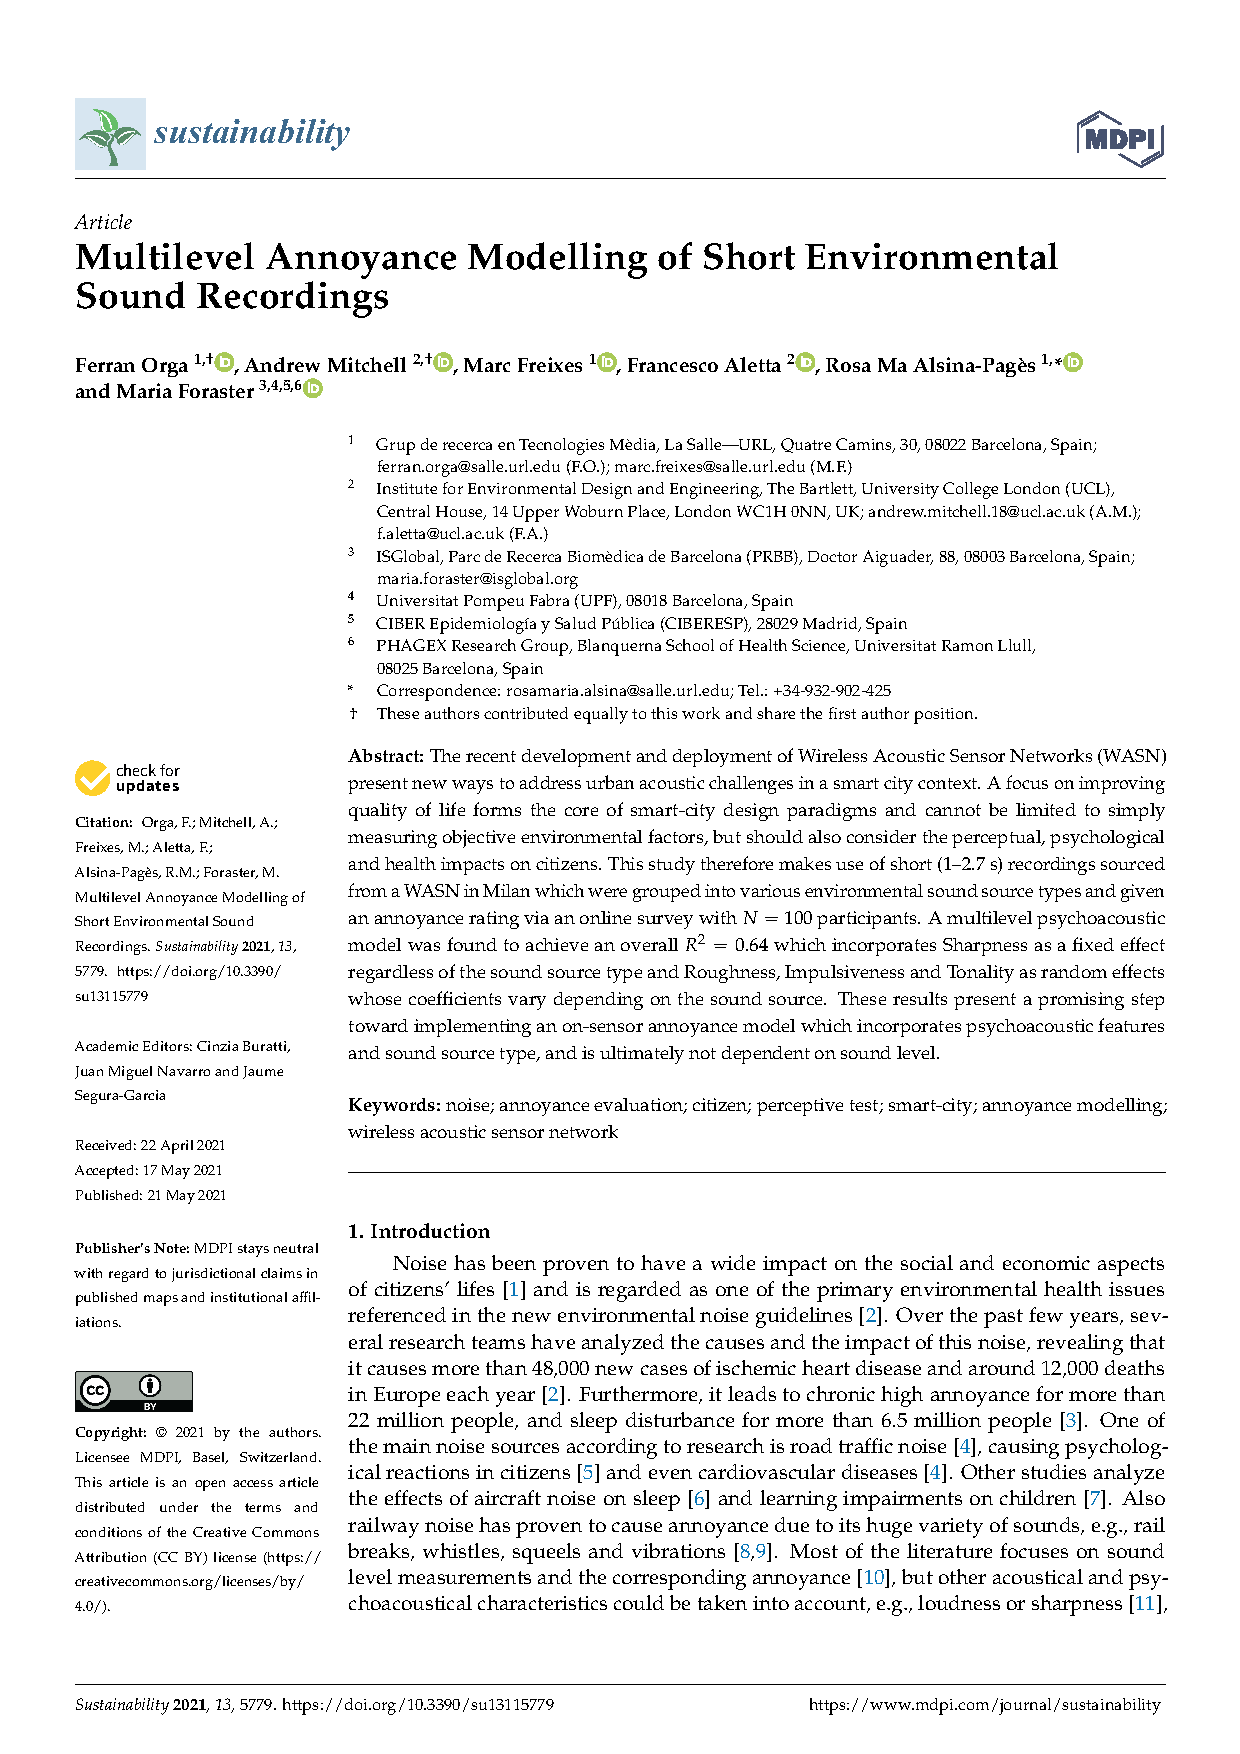
\includepdf[pages=-]{./Papers/Orga2021Multilevel.pdf}

\chapter[Study III: Predictive Soundscape Modelling of the Lockdowns]{Investigating Urban Soundscapes of the COVID-19 Lockdown: A predictive soundscape modelling approach}

This paper is part of a special issue on COVID-19 Pandemic Acoustic Effects.

\section*{Abstract}
 The unprecedented lockdowns enforced around the world to fight COVID-19 in spring 2020 triggered changes in human activities in public spaces. A predictive modelling approach was developed to characterise the resulting change in the perception of the sound environment when people could not be surveyed. Building on a database of soundscape questionnaires ($N = 1,318$) and binaural recordings ($N = 693$) collected in 13 locations across London and Venice during 2019, new recordings ($N = 608$) were made in the same locations during the lockdowns in 2020. Using these 30-second-long recordings, linear multi-level models were developed to predict the pleasantness and eventfulness of the soundscapes during the lockdown and compare changes for each location. An online listening study also investigated the change in sound sources within the spaces. Results indicate:

 \begin{enumerate}
   \item human sounds were less dominant and natural sounds more dominant across all locations
   \item contextual information is important for predicting pleasantness but not for eventfulness
   \item in general, perception shifted towards less eventful soundscapes and to more pleasant soundscapes for traffic-dominated locations, but not for human- and natural-dominated locations.
 \end{enumerate}

 This study demonstrates the usefulness of predictive modelling and the importance of considering contextual information when discussing the impact of sound level reductions on the soundscape.

\section{Introduction}
 \label{sec:intro}
 The global emergency cause by the \gls{covid19} in early 2020 required national lockdown measures across the world, primarily targeting human activity. In the United Kingdom, construction and transport were allowed to continue, but a decrease in activity was observed \citep{Hadjidemetriou2020impact}. In other countries, such as Italy, the restrictions were more severe and even included limiting people's movement to a certain radius from their place of residence \citep{Ren2020Pandemic}. The explorations in environmental acoustics of lockdown conditions across the world have revealed various degrees of impact on the acoustic environment, both at a city-scale \citep{Asensio2020Changes,BonetSola2021Soundscape,Hornberg2021Impact,Munoz2020Lockdown,Rumpler2021Noise} and at a more local, public space-scale \citep{Aletta2020Assessing,AlsinaPages2021Changes,BonetSola2021Soundscape,VidaManzano2021sound}. In general, these studies have demonstrated a decrease in urban noise levels and indicated a difference in the amount of decrease depending on the type of space investigated (e.g. parks, urban squares, etc.) and the type of human activity characteristic for the space.

 Those studies were mostly focussed around the \gls{laeq}, as well as a standardization approach to reporting subsequent changes in soundscape proposed by \citet{Asensio2020Taxonomy}. They were not able to reveal the perceptual impact of such conditions in public spaces as well because of: 1) the lack of subjective data for the exact or comparable locations in previous years; and 2) the lack of participants present in public spaces during the lockdown, hence the ability to collect soundscape data in-situ. Attempts have been made to bridge this gap by using social networks to source subjective data, but this resulted in a focus on indoor conditions following the shift in the citizens' behaviour, i.e. spending more time indoors \citep{Bartalucci2021survey,Lee2021Attitudes}. \citet{GarridoCumbrera2021Perceptions} relied on an online survey deployed in England, Ireland, and Spain to explore the perceived change in natural environments in particular. They observed a consistent increase in the perceived presence of natural sounds across all major cities and rural areas respectively in these three countries. A very similar trend was observed in Argentina, also based on an online questionnaire without a listening task \citep{Maggi2021Perception}. By combining field recordings and focus groups, \citet{Sakagami2020How} and \citet{Lenzi2021Soundscape} observed changes in the sound source composition and the affective quality of soundscape in a residential area in Kobe, Japan and a public space in Getxa, Spain, respectively, during the different stages of the lockdown period. Following the easing of lockdown measures, a decrease in animal and traffic sounds was observed in Kobe, while an increase in eventfulness, loudness, and presence of human sound sources, followed by a decrease in pleasantness, was shown in Getxa.

 \citet{Aletta2020Assessing} explored the impacts of the \gls{covid19} lockdowns on the acoustic environment in London in particular, through many short-term (30s) binaural recordings. This study revealed that average reductions in the various locations considered ranged from 10.7 dB (\gls{laeq}) to 1.2 dB, with an overall average reduction of 5.4 dB. This metric-reporting focussed approach left the following research questions unanswered:
 \begin{enumerate}
   \item How would people have perceived these spaces as a result of this change in acoustic environment? (RQ1)
   \item Would these sound level reductions result in improvements to the soundscape of the spaces? (RQ2)
 \end{enumerate}

 The \nth{1} research question (RQ1), addressing the perceptual effect of the change in urban soundscape induced by the lockdowns, can be further broken down into the following questions:

 \begin{itemize}
   \item How was the sound source composition influenced by the change?
   \item How would the affective response to the acoustic environment in lockdowns change?
   \item Could this demonstrate the effect of human activities on the perception of an acoustic environment in general?
 \end{itemize}

 These questions arise out of the soundscape approach, which is characterised by prioritising the perceptual effect of an acoustic environment by taking into account the interaction of sound sources, context, and the person perceiving it \citep{ISO12913_1_2014IOS} \cit{truax1999}, bringing together objective and subjective factors. The soundscape approach to noise mitigation and management is being recognised as a response to arising environmental requirements on noise pollution and sustainability, such as the regulation of quiet areas in Europe \citep{EEA2020Environmental, Aletta2018Towards} \cit{Radicchi2021}. This has been further formalised in \citet{ISO12913_2_2018IOS} via the adoption of the circumplex model of soundscape \citep{Axelsson2010principal}, in which the perception of a soundscape can be described in terms of its pleasantness and eventfulness, as one of the standard methods of soundscape assessment.

 Soundscape research is therefore traditionally rooted in environmental acoustics and environmental psychology, typically dealing with outdoor spaces \citep{Torresin2020Indoor} and urban open spaces, where parks and squares are often used as case study sites \cit{Kang 2007}. A soundscape assessment typically requires people to be surveyed but the presence of people at a location influences assessment \citep{Aletta2018Towards} and 'quiet places' usually require low numbers of users to remain quiet, which limits the possibility of an assessment. Even in a crowded public space, soundscape surveys are demanding as they require significant resources to carry out at scale, limiting their widespread application \citep{Mitchell2020Soundscape}. Therefore, a need for a predictive model arises to overcome this limitation and improve the implementation of the soundscape approach into everyday planning and management practices.

 According to a recent review of predictive soundscape models from \citet{Lionello2020systematic}, the degree of employing auditory and non-auditory factors in soundscape prediction varies with some studies relying on contextual \citep{Kajihara2017Imaginary}, personal/demographic \citep{Erfanian2021Psychological} \cit{tarlao2021} or social media \citep{Aiello2016Chatty} data entirely to predict and generate soundscape features. Some methods also incorporate perceptually-derived features, such as subjective sound level and visual pleasantness as predictors \citep{Lionello2020systematic}, however this information must also be obtained from people via a survey and therefore are unsuitable for predictive modelling where surveys are not possible. This indicates the necessity for considering and accounting for the influence which contextual factors in a space have on the relationship between the sound environment itself and the listener's perception of it (i.e. the soundscape).

 Therefore, a third research question arises: what are the key features needed for a soundscape prediction model based on comprehensive acoustic on site measurements to be used for assessing locations with low social presence or in situations where conducting surveys is impractical (RQ3)?

\section{Materials and Methods}

 This study was conducted via initial onsite data collection campaigns in Central London and Venice in 2019 before the outbreak of \gls{covid19} as part of the \gls{ssid} project \citep{Mitchell2020Soundscape} and in 2020 during the strictest part of the lockdowns \citep{Aletta2020Assessing}, including objective acoustic data (2019 and 2020) and subjective responses (2019 only). Using both 2019 and 2020 binaural recordings, an online listening experiment was conducted to provide an understanding about the change in sound source composition. The 2019 onsite questionnaire data were used to define the dominant sound source at each location as a starting point for interpreting the soundscape change. A predictive model was developed to reveal the change in the perceived pleasantness and eventfulness using objective acoustic data and location to predict subjective responses. Although the initial (2019) dataset contains additional locations (specifically, in Spain, the Netherlands, and China), due to the nature of this study as a reaction to the strict movement and activity restrictions, the sites which could be included in the lockdown (2020) measurement campaigns were limited to locations where staff and equipment had access and where recordings could be undertaken during the spring of 2020.

 The sites were selected to provide a mixture of sizes and uses, varying in typology ranging from paved squares to small and large parks to waterside spaces across both cities. Throughout the text they are indexed via a LocationID based on the location's name (e.g. CamdenTown, SanMarco), while a more in-depth overview of each is given in supplementary files. %NOTE: Will need to adjust this within thesis.
 London is taken as an example of a large, typically noisy city while the Venice sample provides a unique look at spaces with typically very high human activity levels and no road traffic activity. In particular, the 2019 Venice surveys were taken to coincide with the yearly Carnevale festival in order to capture its distinct soundscape.

 The ISO/TS 12913 \citep{ISO12913_2_2018IOS} series were consulted for reporting on soundscape data. A detailed description of the 2019 survey campaigns in featured through the paper and in the supplementary files. This study was approved by departmental UCL IEDE Ethics Committee on \nth{17} July 2018 for onsite data collection and on the \nth{2} of June 2020 for the online listening experiment and is conducted in adherence to the ethical requirements of the Declaration of Helsinki \citep{WMA2013World}.

 \subsection{Onsite data: Questionnaires, binaural measurements, and recordings}
   %FIXME: Likely will not need this within thesis.
   The initial onsite data collection featured both questionnaire data collected from the general public and acoustic measurements, conducted across thirteen urban locations (in London $N=11$, in Venice $N=2$) between the \nth{28} of February and the \nth{21} of June 2019, with additional sessions in July and October 2019. A total of 1,318 questionnaire responses were collected from the general population across the measurement points during 1 -- 3 hour-long campaigns in both cities in 2019, accompanied by 693 approximately 30-second long 24-bit 44.1 kHz binaural recordings. Each of the 13 locations was characterised by between 14 to 80 recordings and between 32 to 155 questionnaire responses. Mean age of the participants was 33.9 (45\% male, 53.8\% female, 0.4\% non-conforming, 0.9\% prefer-not-to-say).

   The subsequent measurement campaign in 2020 mimicked the binaural recording strategy applied in the initial campaign and was performed between the \nth{6} and the \nth{25} of April 2020 in both cities, this time excluding the questionnaire. An additional 608 binaural recordings were collected on site in 2020.

   \subsubsection{Data collection}
   %FIXME: Probably don't need this section in thesis either.
   The 2019 data collection was performed across all the locations using the protocol based on the Method A of the ISO/TS 12913-2:2018 \citep{ISO12913_2_2018IOS}, as described in \citep{Aletta2020Assessing,Mitchell2020Soundscape}, collected either via handheld tablets or paper copies of the questionnaire. The full questionnaire and data collection procedure are given in \citet{Mitchell2020Soundscape}, however the key parts used for this study are those addressing sound source dominance and \gls{paq}.
   %NOTE: Skipping next section since it's detailed earlier in thesis.

   %NOTE: add a section to the methods about the projection. Heavy reference to / pulling from Lionello 2020 and JASA-EL paper.
   In order to simplify the results and allow for modelling the responses as continuous values, the 8 \gls{paq}s undergo a trigonometric projection to reduce them onto the two primary dimensions of pleasant and eventful, according to the procedure outlined in Part 3 of the ISO 12913 series \citep{ISO12913_3_2019IOS}. In order to distinguish the projected values from the Likert-scale \gls{paq} responses, the projected values will be referred to as \gls{isopl} and \gls{isoev} and can be considered to form an x-y coordinate point (x = \gls{isopl}, y = \gls{isoev}) as explained in detail in \citet{Lionello2021Introducing}.

   %NOTE: Skipping paragraph on binaural recording info

   \subsubsection{Data cleaning}
   %TODO: Move and expand this data cleaning section to the methods section
   The cleaning of the samples was conducted using the ArtemiS SUITE 11. The researcher discarded or cropped whole recordings, or its parts affected by wind gusts or containing noises and speech generated by the recording operator by accident or for the purpose of explaining the questionnaire to a participant. This resulted in 1,291 binaural recordings which were then processed further, as described in Section \ref{sec:analyses}. Psychoacoustic analyses are shown in supplementary files.

   In order to maintain data quality and exclude cases where respondents either clearly did not understand the \gls{paq} adjectives or intentionally misrepresented their answers, surveys for which the same response was given for every \gls{paq} (e.g. 'Strongly agree' to all 8 attributes) were excluded prior to calculating the ISO projected values. This is justified as no reasonable respondent who understood the questions would answer that they 'strongly agree' that a soundscape is pleasant and annoying, calm and chaotic, etc. Cases where respondents answered 'Neutral' to all \gls{paq}s are note excluded in this way, as a neutral response to all attributes is not necessarily contradictory. In addition, surveys were discarded as incomplete if more than 50\% of the \gls{paq} and sound source questions were not completed.
   %TODO: Update ISO citations to what we did in the ASA submission, that was better.
   The site characterisation per \citet{ISO12913_2_2018IOS} is available in the supplementary files, featuring the address, overall psychoacoustic characteristics of the location, typical use of each location, and pictures taken during the survey sessions.

   \subsubsection{Psychoacoustic analyses}
   \label{sec:analyses}
   %NOTE: May want to move this to methods as well.
   The binaural recordings were analysed in ArtemiS SUITE 11 to calculate the following suite of 11 acoustic and psychoacoustic features to be used as initial predictors:

   \begin{enumerate}
     \item Loudness (\gls{n5}, sones, per ISO 532-1:2017)
     \item Sharpness (\gls{s}, acum, per ISO 532-1:2017)
     \item Roughness (\gls{r}, asper)
     \item Impulsiveness (\gls{iu})
     \item Fluctuation Strength (\gls{fs}, vacil)
     \item Tonality (\gls{tu}, tuHMS)
     \item Zwicker Psychoacoustic Annoyance (\gls{pa}, per \citet{PsychoacousticsZwicker})
     \item \gls{laeq}, 30s (dB)
     \item \gls{la10la90} (dB)
     \item \gls{lcla} (dB)
     \item Relative Approach (\gls{ra}, per \citet{Genuit1996Objective})
   \end{enumerate}

   The (psycho)acoustic predictors investigated were selected in order to describe many aspects of the recorded sound -- in particular, the goal was to move beyond a focus on sound level, which currently dominates the existing literature on the acoustic effects of lockdowns noted in Section \ref{sec:intro}. In all, they are expected to reflect the sound level (\gls{laeq}), perceived sound level (\gls{n5}), spectral content (\gls{s}, \gls{lcla}, \gls{tu}), temporal character or predictability (\gls{iu}, \gls{fs}, \gls{ra}), and overall annoyance (\gls{pa}). These metrics have been proposed as indicators to predict perceptual constructs of the soundscape \citep{Aletta2017Dimensions, Aletta2016Soundscape} and have shown promise when combined together to form amore comprehensive model applied to real-world sounds \citep{Orga2021Multilevel}. The maximum value from the left and right channels of the binaural recording are used, as suggest in ISO/TS 12913-3:2019 \citep{ISO12913_3_2019IOS}.

   Table \ref{tab:corr} shows the Pearson correlation coefficient between each of the candidate acoustic features and the outcome pleasantness and eventfulness. For \gls{isopl} ($ISOPl$), we can perhaps see three tiers of correlations:

   \begin{enumerate}
     \item The more highly correlated tier ($|r| > 0.28$) consists of \gls{ra}, \gls{laeq}, \gls{r}, \gls{n5}, and \gls{pa}
     \item The low correlation tier consists of \gls{la10la90}, \gls{tu}, and \gls{iu}
     \item \gls{lcla}, \gls{iu}, and \gls{s} show no correlation
   \end{enumerate}

   For \gls{isoev} ($ISOEv$), these tiers are:
   \begin{enumerate}
     \item The more highly correlated tier ($|r| > 0.30$) consists of \gls{ra}, \gls{laeq}, \gls{tu}, \gls{r}, and \gls{n5}
     \item The low correlation tier consists of \gls{lcla}, \gls{la10la90}, \gls{fs}, and \gls{pa}
     \item \gls{iu} and \gls{s} show no correlation
   \end{enumerate}

   Among the correlations for the psychoacoustic metrics considered for inclusion as input features, we can see several highly inter-correlated features. As expected, \gls{pa}, \gls{laeq}, and \gls{n5} are highly correlated, meaning that careful consideration is paid to these features to ensure they do not contribute to multicollinearity in the final model.

 \subsection{Modelling}

   Two linear multi-level models (MLM) were computed to predict: 1) \gls{isopl}, and 2) \gls{isoev}. The inherent grouped structure of the \gls{ssid} database necessitates a modelling and analysis approach which considers the differing relationships between the objective acoustic features and the soundscape's perceived affective quality ratings across the various locations and contexts. The individual-level of the models is made up of the acoustic features calculated from the binaural recordings made during each respondent's survey period, while the group-level includes the categorical 'LocationID' variable indicating the location in which the survey was taken, acting as a non-auditory contextual factor.

   A separate backwards-step feature selection was performed for each of the outcome models in order to identify the minimal feature set to be used for predicting each outcome. In this feature selection process, an initial model containing all of the candidate features was fit. Each feature was then removed from the model one at a time, then the best-performing model is selected and the procedure continues step-wise until no improvement is seen by removing more features. This process is carried out first on the location-level features (including the potential to remove all features including LocationID, resulting in a 'flat' or standard multivariate linear regression model), then on the individual-level features. The performance criterion used for this process was the \gls{aic} \citep{Akaike1974New}. To check for multicollinearity among the selected features, the \gls{vif} was calculated and a threshold of $\gls{vif} < 5$ was set. Any features which remained after the backwards step-wise selection and which exceeded this threshold were investigated and removed if they were highly collinear with the other features.

   All of the input features are numeric values, in the units described above. Before conducting feature selection, the input features are z-scaled to enable proper comparison of their effect sizes. After the feature selection, the scaled coefficients are used in the text when reporting the final fitted models to facilitate discussion and comparison between the features. The unscaled model coefficients are reporting in \draft{Appendix B} to enable the models to be applied to new data. In order to properly assess the predictive performance of the model, an 80/20 train-test split with a balanced shuffle across LocationIDs was used. The z-scaling and feature selection were performed on the training set only, in order to prevent data leakage. To score the performance of the model on the training and testing sets, we use the \gls{mae}, which is in the scale of the response feature -- for \gls{isopl} and \gls{isoev} this means our response can range from $-1$ to $+1$. However, since the end-goal of the model is to predict the soundscape assessment of the location as a whole, rather than the individual responses, we also assess the performance of the model in predicting the average response in each location. To do this, the mean response value for each location is calculated, and the $R^2$ accuracy across LocationIDs is reported for both the training and testing sets.

   The model fitting and feature selection was performed using the `step` function from `lmerTest` (v3.1.3) \citep{Kuznetsova2017lmerTest} in R statistical software (v.4.0.3) \citep{RCT2021R}. The summaries and plots were created using the `sjPlot` package (v.2.8.6) \citep{Luedecke2021sjPlot} and `seaborn` (v.0.11.1) \citep{Waskom2021seaborn}.

 \subsection{Online Survey}

   A online listening test was conducted using the Gorilla Experiment Builder \href{www.275gorilla.sc}{} \citep{AnwylIrvine2020Gorilla}. The participants were exposed to a random selection of 78 binaural recordings (39 from 2019 and 39 from 2020, 6 recordings per location). Each participant had the option to evaluate either 1 or 2 sets of 6 recordings randomly assigned between 13 stimuli sets. Mp3 files, converted at 256 kBps were used due to the requirements of the Gorilla platform.

   No visual stimuli were used in the experiment. The experiment consisted of:

   \begin{enumerate}
     \item an initial exercise to enhance the chances of participants complying with the instructions and wearing headphones
     \item a training set using two randomly chosen binaural recordings (then not used in the main task) from the dataset
     \item a soundscape characterisation questionnaire starting with an open-ended question about perceived sound sources and featuring the same questions as the one used in-situ, looking into the perceived sound source dominance of the following four types: traffic noise, other noise, human sounds, and natural sounds
     \item a questionnaire on the basic demographic factors.
   \end{enumerate}

   The questionnaire used in Part 3 of the online experiment is report in \draft{Appendix A}.

   Having in mind the remote nature of the study and to ensure a minimum level of robustness for reliable sound source recognition, an initial exercise was performed consisting of a headphone screening test \citep{Woods2017Headphone} and a headphone reproduction level adjustment test \citep{Gontier2019Estimation}. The level adjustment was performed using an 11-second-long pink noise sample matched to the lowest and the highest \gls{la90} values from the experimental set. Participants were asked to adjust their listening level to clearly hear the quieter sample while keeping the level low enough, so they don't find the louder sample disturbing. The headphone screening test followed, featuring a stereo signal of 1-second-long 100 Hz sin tone, generated with Izotope RX6 application, played at a 3 dB difference where one of the equally loud pairs had its phase inverted. A 100 Hz sin was used because the pilot tests revealed that the 200 Hz sin tone proposed by \citet{Woods2017Headphone} created a higher uncertainty varying across different laptop models and would likely contribute to the chances of a participant fooling the test. It was expected that participants using speakers would not be able to either hear the sin wave or would be fooled by the inverted phase effect and therefore not able to pass the trials, unless they were indeed using headphones. The participant needed to recognise the quietest of the 3 samples in a trial of 6 attempts. Only participants correctly answering 5 or more out of 6 trials were allowed to proceed with the experiment. Participants were asked not to change their audio output settings during the rest of the experiment. This was introduced to ensure that a participant is using a headphone playback system which allows a listener to clearly recognise a 3 dB difference at 100 Hz as a proxy for sufficient audio quality playback.

   Online questionnaire data was collected between the \nth{9} of June and the \nth{9} of August 2020. Within the Gorilla Experiment Builder, a total of 250 attempts to complete the experiment were recorded, where 165 participants were excluded either on the basis of not passing the headphone screening ($N=79$) or for not completing the experiment, usually before engaging into the screening ($N=83$). Out of a total of 88 participants who completed the test, 2 participants were excluded as outliers as they provided uniform answers across all the questions and commented on not being able to properly hear the stimuli, despite their successful completion of the training tests. The participants of the online experiment were of mean age 32.42, 45.1\% male, 54.9\% female.

   Figure \ref{fig:lockdown-study-framework} illustrates and summarises the framework and sections described above.

   \begin{figure}
     \label{fig:lockdown-study-framework}
     \centering
     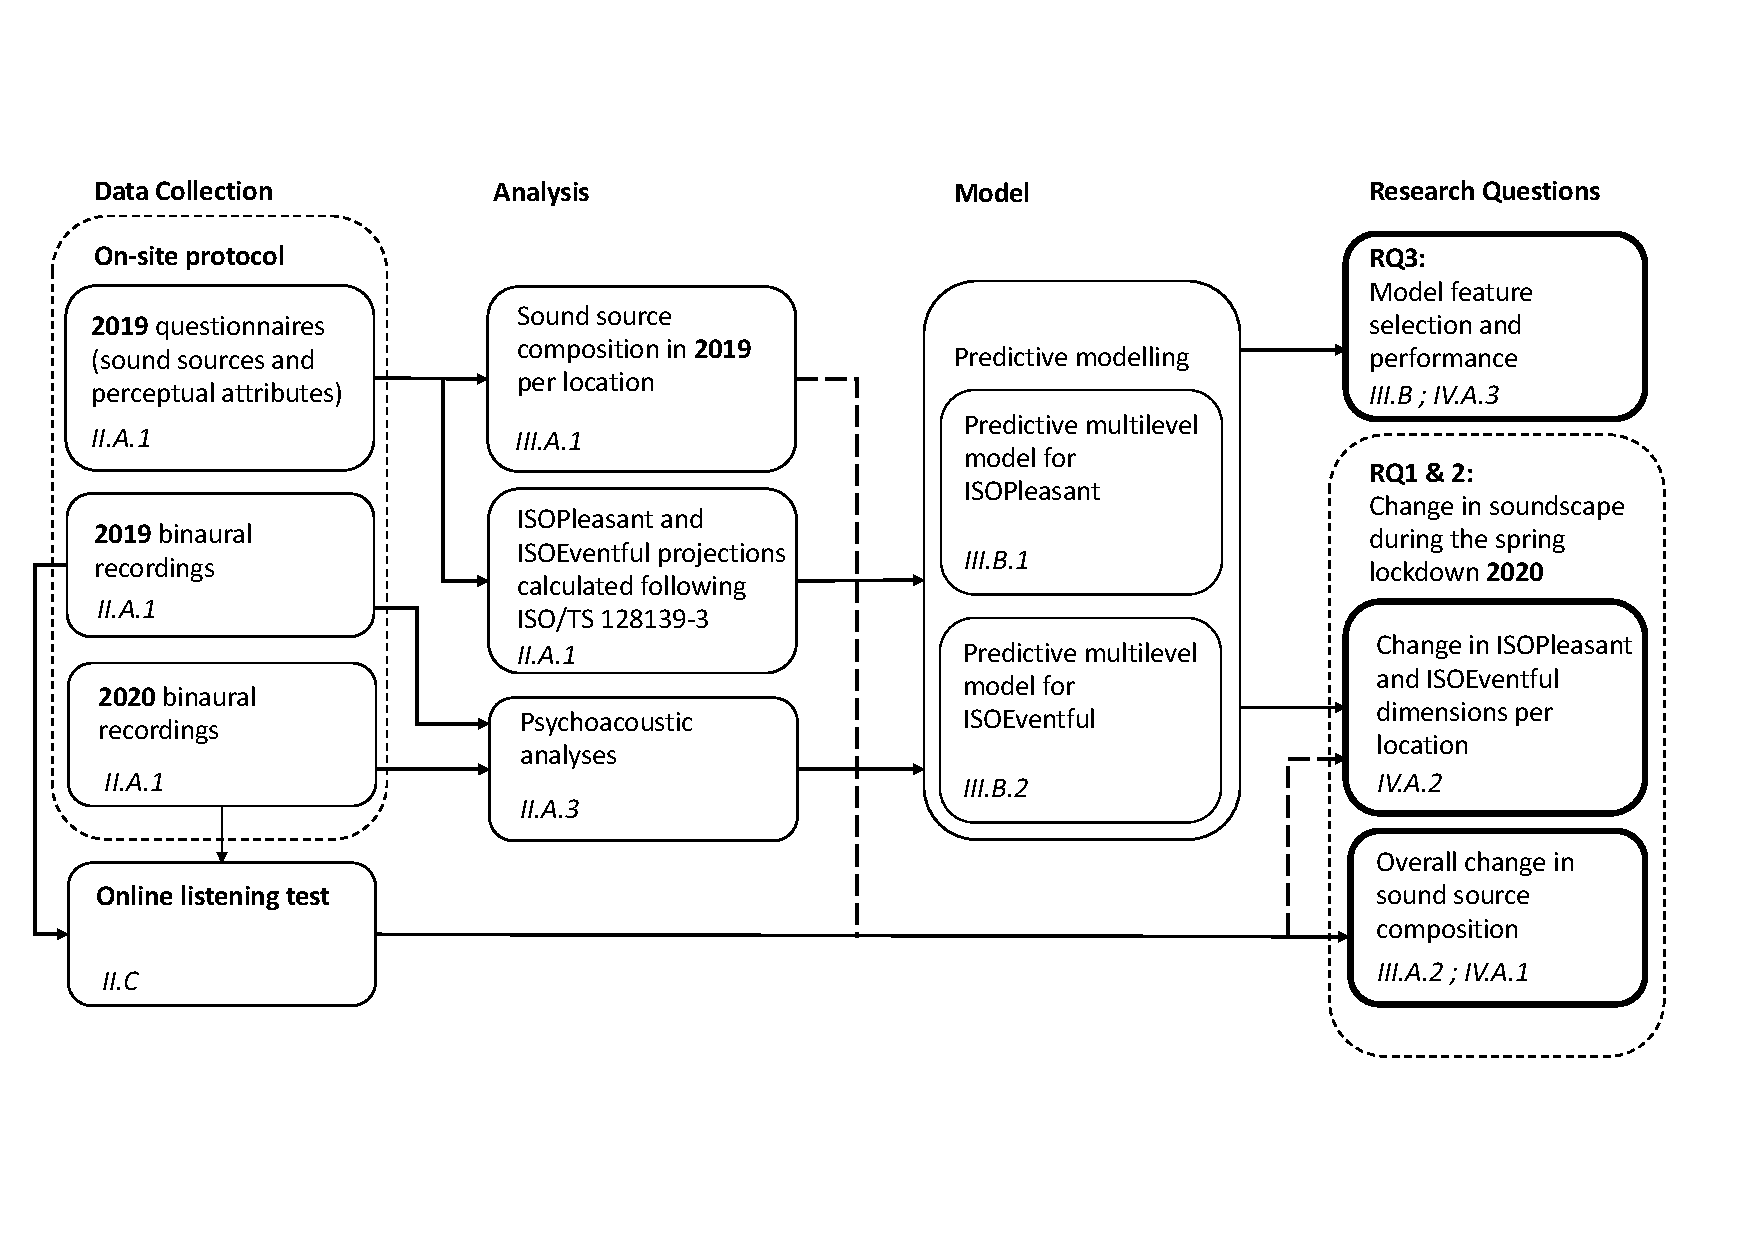
\includegraphics[width=\textwidth]{Figures/Lockdown-Fig1.pdf}
     \caption{The study flowchart indicating the data collection, analysis, modelling, and discussion throughout the study. The subsections in the text to which each box refers are indicated in italics.}
     %FIXME: Change the section references to match.
   \end{figure}

\section{Results}

 The results of the onsite surveys, online experiment, and the model development are reported here. They are reported following the structure of the ISO/TS 12913 series, revealing the perceived sound source dominance, key perceptual attributes (\gls{isopl} and \gls{isoev}) and the lockdown-related changes.

 \subsection{Perceived sound source dominance}

   \subsubsection{2019 sound source composition per location}

   Questionnaire data was collected English, Italian, and Spanish in both cities. The respective questionnaires can be found in the supplementary files and \citet{Mitchell2020Soundscape}. Data presented here was aggregated per LocationID.

   According to the highest scored mean value of the dominant sound source type, as show in Figure \ref{fig:sound-source-dom}, the locations can be grouped into: natural sounds dominated (RegentsParkJapan, RegentsParkFields, RussellSq), human sounds dominated (SanMarco, TateModern, StPaulsRow, StPaulsCross, MonumentoGaribaldi), noise (traffic and other noise) sounds dominated (CamdenTown, EustonTap, TorringtonSq, PancrasLock).

   \begin{figure}
     \label{fig:sound-source-dom}
     \centering
     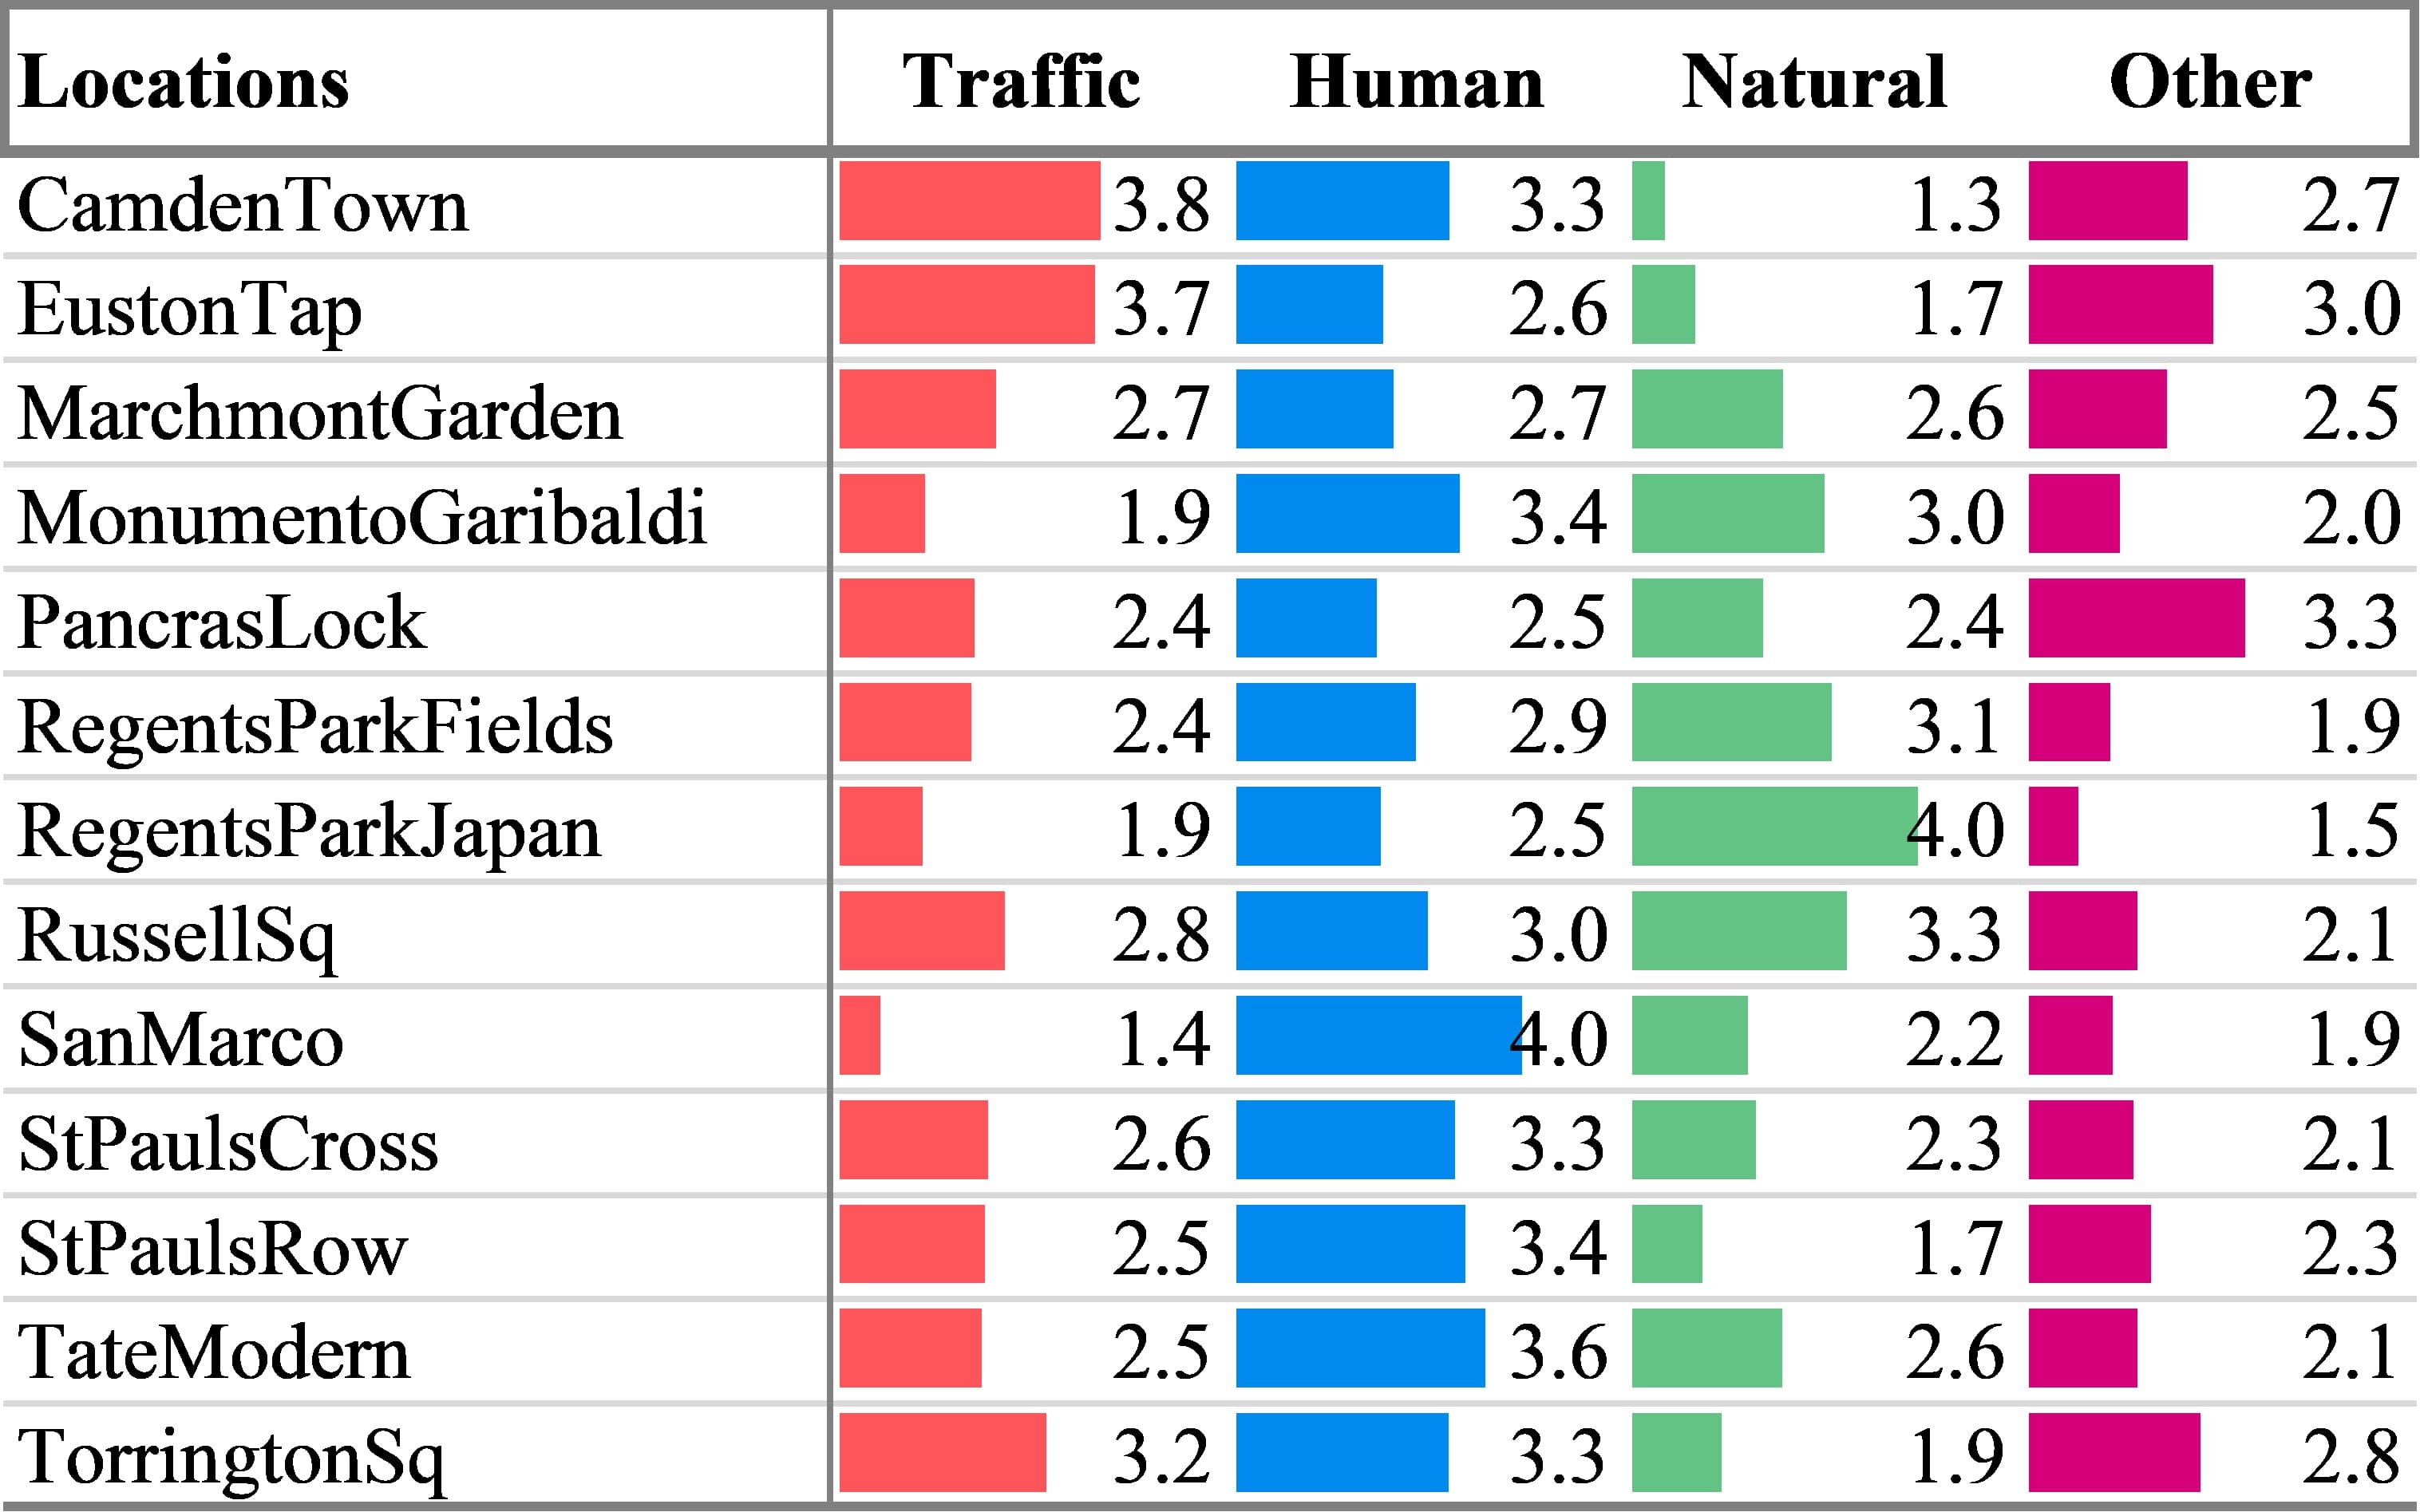
\includegraphics[width=.8\textwidth]{Figures/Lockdown-Fig2.jpg}
     \caption{Mean values per LocationID for the perceived dominance of the sound source types, for the 2019 on-site campaign.}
   \end{figure}

   \subsubsection{Overall change in the perceived sound source dominance during lockdown}

   1,803 words describing the sound sources present in the 2019 recordings and 1,395 words related to the 2020 recordings were input by participants in response to the open-ended question Q1 \draft{(see Appendix A)}. The frequency of occurrence, generated using the Word-Clouds web app, is shown in Figure \ref{fig:wordclouds}, for the 2019 and the 2020 sets respectively. The most frequency words from both 2019 and 2020 groups are: noise, car/traffic, bird/birds, talk/voice, and (foot)steps.

   \begin{figure}
     \label{fig:wordclouds}
     %TODO: add wordcloud figure
   \end{figure}

   The results from the listening tests deployed online were analysed using SPSS Statistics v. 25. Levene's test for equality of variances resulted in highly statistically significant values for all 4 sound sources investigated ($<0.001$). Therefore, a Mann-Whitney U-test was used as a non-parametric equivalent to the t-test to investigate the change in the perceived dominance of the four sound source types \citep{McKnight2010Mann}. The results for human sounds indicated that the perceived dominance was greater for the 2019 sample ($M=3.82$) than for the 2020 sample ($M=2.62, U=41,656, p<0.001$). The results for natural sounds indicated the perceived dominance increased from 2019 ($M=2.00$) to 2020 ($M=2.54, U=63,797, p<0.001$). However, the differences for the noise sources (traffic and other) were not statistically significant.

   \begin{figure}
     \label{tab:source-dominance-stats}
   \end{figure}

 \subsection{Model selection, performance, and application}

   \subsubsection{\gls{isopl} model selected}

   Following the feature selection, the \gls{isopl} model (given in Table \ref{tab:scaled-model}) has \gls{n5} as the fixed effect with a scaled coefficient of -0.06, and \gls{laeq}, \gls{la10la90}, and \gls{lcla} as coefficients which vary depending on the LocationID. The training and testing \gls{mae} are very similar, indicating that the model is neither over- nor under-fitting to the training data ($MAE_{train}=0.259, MAE_{test}=0.259$). The model performs very well at predicting the average soundscape assessment of the locations ($R^2_{train}=0.998, R^2_{test}=0.85$).

   \begin{table}
     \label{tab:scaled-model}
     \caption{Scaled linear regression models of \gls{isopl} and \gls{isoev} for 13 locations in London and Venice. The \gls{isopl} model is a multi-level regression model with one level for individual effects and a second level for LocationID effects, while the \gls{isoev} model is a 'flat' multi-variate linear regression with no location effects.}
   \end{table}

   The high intraclass correlation ($ICC=0.90$) demonstrates that the location-level effects are highly important in predicting the pleasantness dimension. Within this random-intercept random-slope model structure, these effects include both the specific context of the location (i.e. the LocationID factor), but also the \gls{laeq}, \gls{la10la90}, and \gls{lcla} features whose effects vary across locations. These slopes are given in Figure \ref{fig:pl-slopes}. This point highlights the need to consider how the context of a location will influence the relationship between the acoustic features and the perceived pleasantness.

   \begin{figure}
     \label{fig:pl-slopes}
     \caption{Location-level scaled coefficients for the \gls{isopl} model.}
   \end{figure}

   \subsubsection{\gls{isoev} model selected}

   Through the group-level feature selection, all of the group-level coefficients, including the LocationID factor itself. Therefore the final \gls{isoev} model is a 'flat' multi-variate linear regression model, rather than a multi-level model. The \gls{isoev} is a linear combination of \gls{s}, \gls{fs}, \gls{tu}, \gls{laeq}, and \gls{lcla}. The training and testing \gls{mae} are very similar, indicating that the model is not over-fit to the training data ($MAE_{train}=0.233; MAE_{test}=0.231$). The model performs slightly worse than the \gls{isopl} at predicting the mean location responses, but still performs well ($R^2_{train}=0.873; R^2_{test}=0.715$).

   \subsubsection{Application to lockdown data}
   %FIXME: Figure out how to do sub-figure referencing
   Once the two models were built and assessed, they were then applied to the lockdown recording data in order to predict the new soundscape ISO coordinates. Figure \ref{fig:circumplex-locations}(a) shows the pre-lockdown ISO coordinates for each location and Figure \ref{fig:circumplex-locations}(b) shows how the soundscapes are predicted to have been assessed during the lockdown period. As in the model assessment process, the predicted responses are calculated for each recording individually, then the mean for each location is calculated and plotted on the circumplex.

   In 2019 the majority of locations in the dataset fall within the 'vibrant' quadrant of the circumplex, particularly those which are primarily dominated by human activity (e.g. SanMarco, TateModern). CamdenTown and EustonTap, which are both in general visually and acoustically dominated by traffic, are the only two to be rated as 'chaotic', while no locations are overall considered to be 'monotonous'. During the 2020 lockdown, there is a general positive move along the 'pleasant' dimension and a general negative move along the 'eventful' dimension, but several patterns of movement can be noted. These are investigated further in the Discussion section below.

   \begin{figure}
     \label{fig:circumplex-locations}
     \caption{Soundscape circumplex coordinates for (a) the mean \gls{isopl} and \gls{isoev} responses for each location; and (b) the mean predicted responses based on recordings made during the lockdown and the location's movement in the circumplex.}
   \end{figure}

   %%%%%%%%%%%%%%%%%%%%%%%%%%%%%%%%%%%%%%%%%%%%%%%%%%%%%%%%%%%

\section{Discussion}

 \subsection{Interpretation of the results}



%  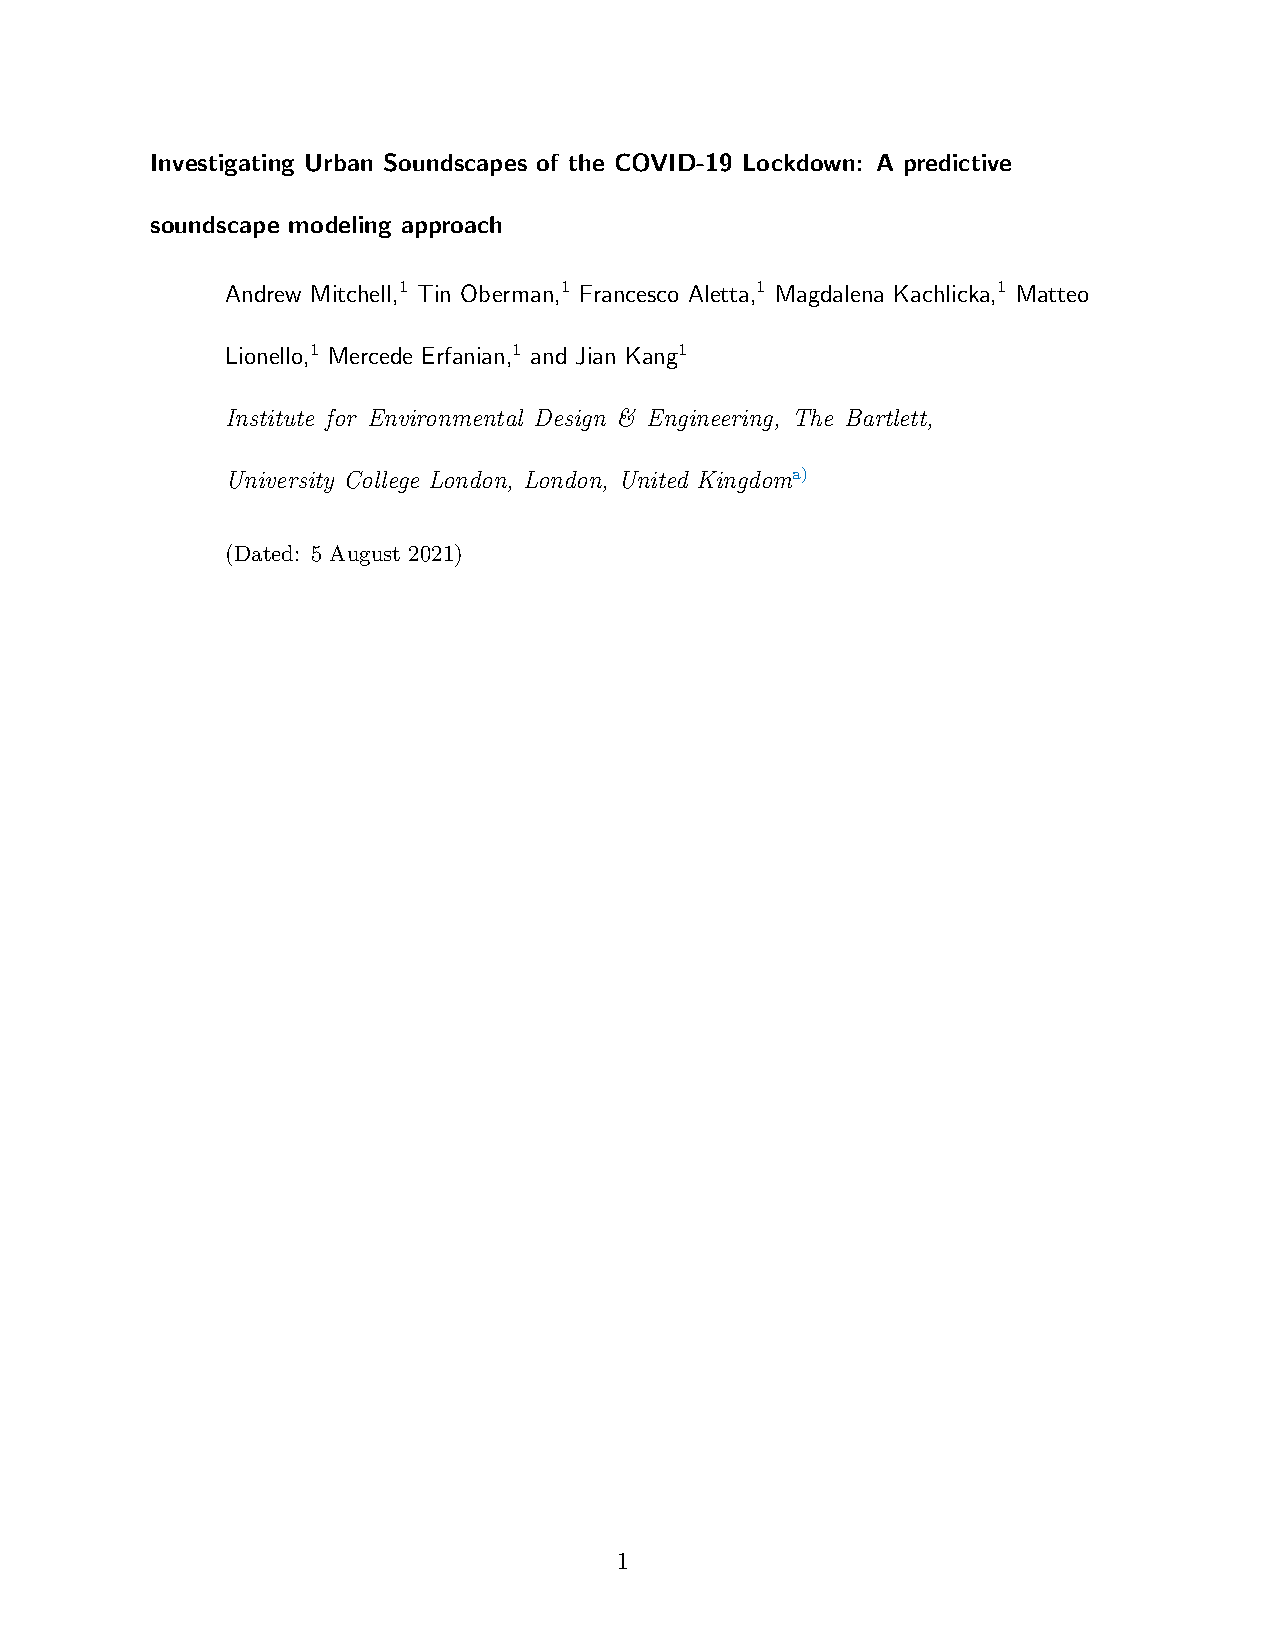
\includepdf[pages=-]{./Papers/Manuscript}

%%%%%%%%%%%%%%%%%%%%%%%%%%%%%%%%%%%%%%%%%%%%%%%%%%%%%%%%%%%%%%%%%%%%%%%%%%%%%%%%%%%%%%%%%%%%%%%%%%%%


\newpage
\chapter[Study IV: DeLTA]{Study IV: A Temporal Convolutional Neural Network for Multi-label Sound Recognition and Annoyance Detection of Complex Soundscapes}

\section*{Background and aims}

 \subsection*{Positivity (or the absence of negativity?)}
       From the experience of the previous studies which are highly focused on the existing environmental acoustic and psychoacoustic metrics, one (of many) potential limitations has been revealed. For the most part, these metrics were designed to characterise various negative qualities of the sound. Certainly, they therefore have a negative correlation with positive assessments of the sound, but the simple fact is that they were conceived of and implemented in an attempt to quantify some sonic characteristic that was assumed by the researchers to contribute to a negative perception. Hence why in Zwicker's empirical formula for Psychoacoustic Annoyance \citep{PsychoacousticsfactsmodelsZwicker} $PA = N_5 (1 + \sqrt{\omega^2_S + \omega^2_{FR}})$, all of the constituent parts have positive coefficients.

       While this would not theoretically hinder a formula for describing positive aspects of the sound, it creates a sort of conceptual barrier. If all of these metrics are designed to capture negative aspects of the sound, then it is insufficient to use them create a formula to describe a positive sound, since that formula would only represent the 'absence of negativity', not necessarily positivity.
\section*{Result and conclusion}

 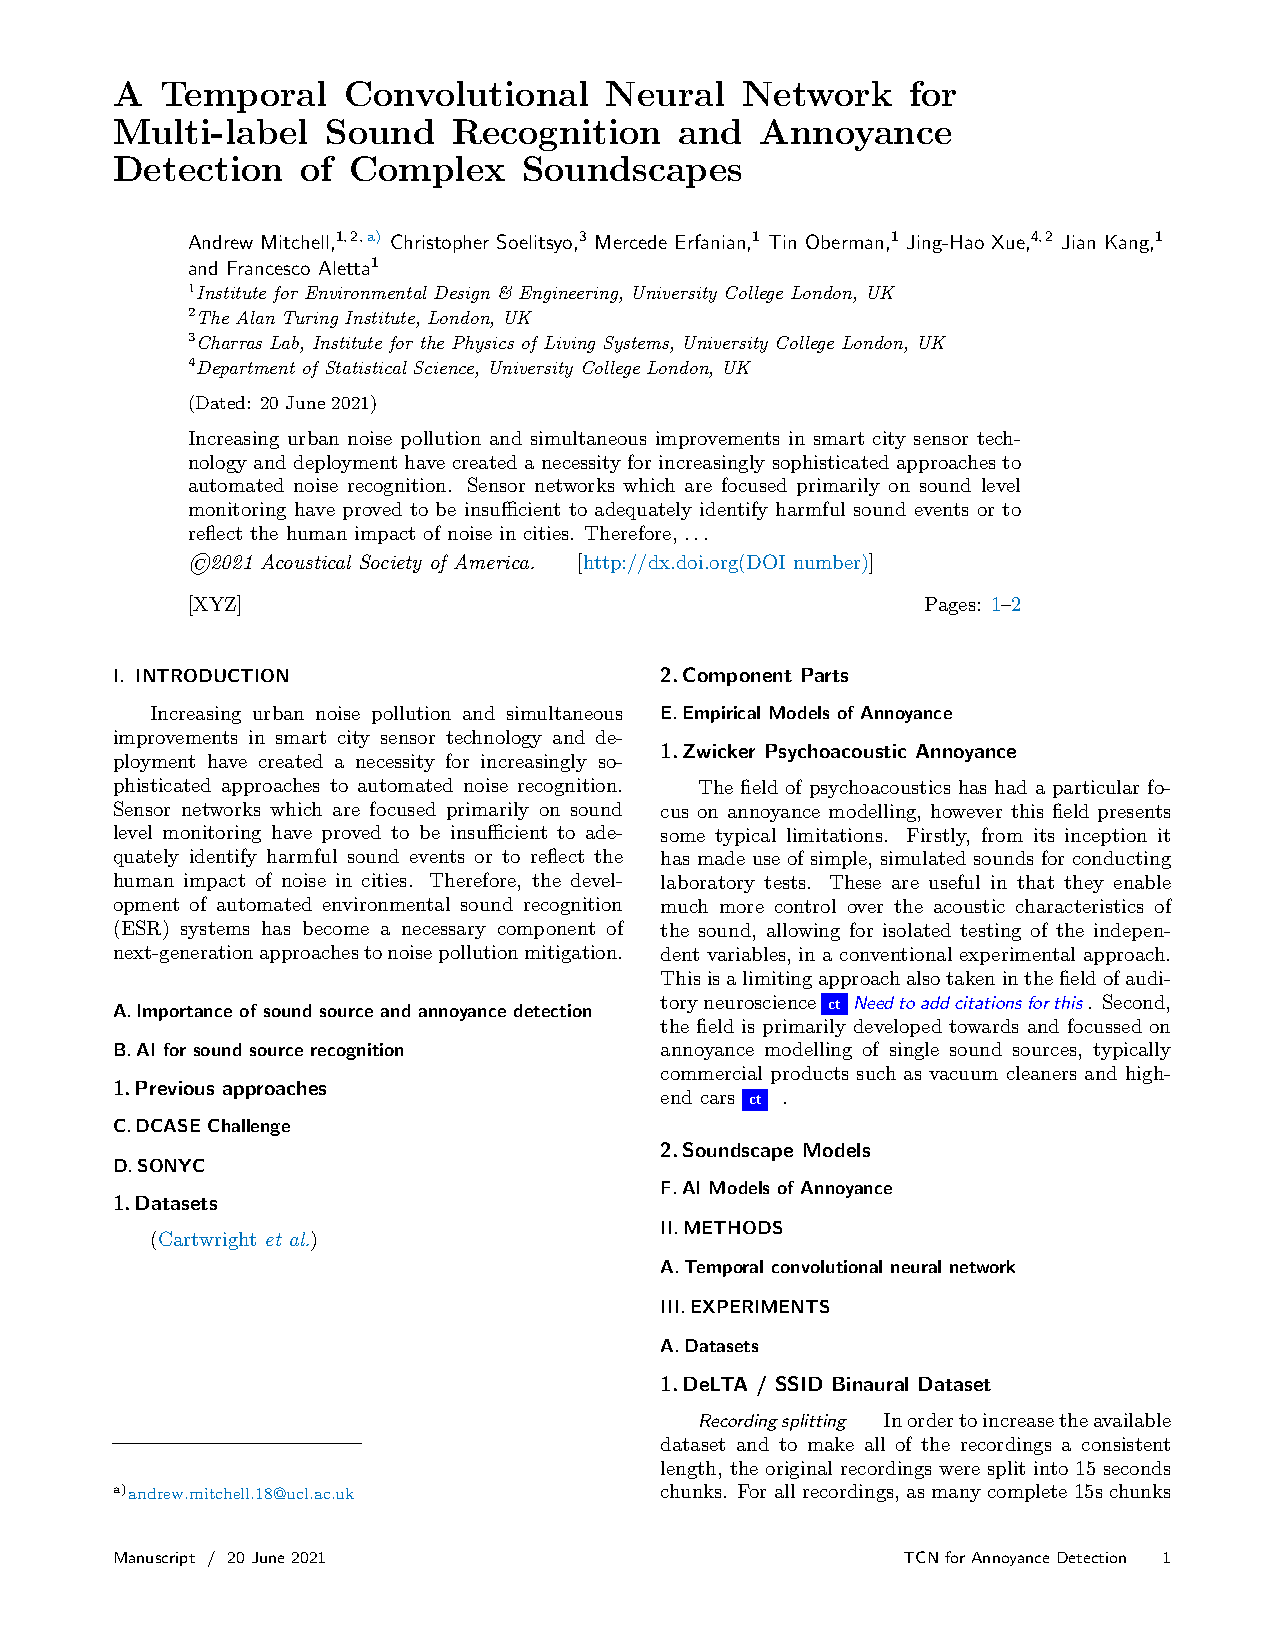
\includepdf[pages=-]{./Papers/IEEE_DeLTA_Preprint.pdf}

 \chapter[Commentary: Probabilistic Soundscapes]{Commentary: From Deterministic to Probabilistic Soundscapes: A critical tour around the soundscape circumplex}

 \hl{Some summary text here.}

 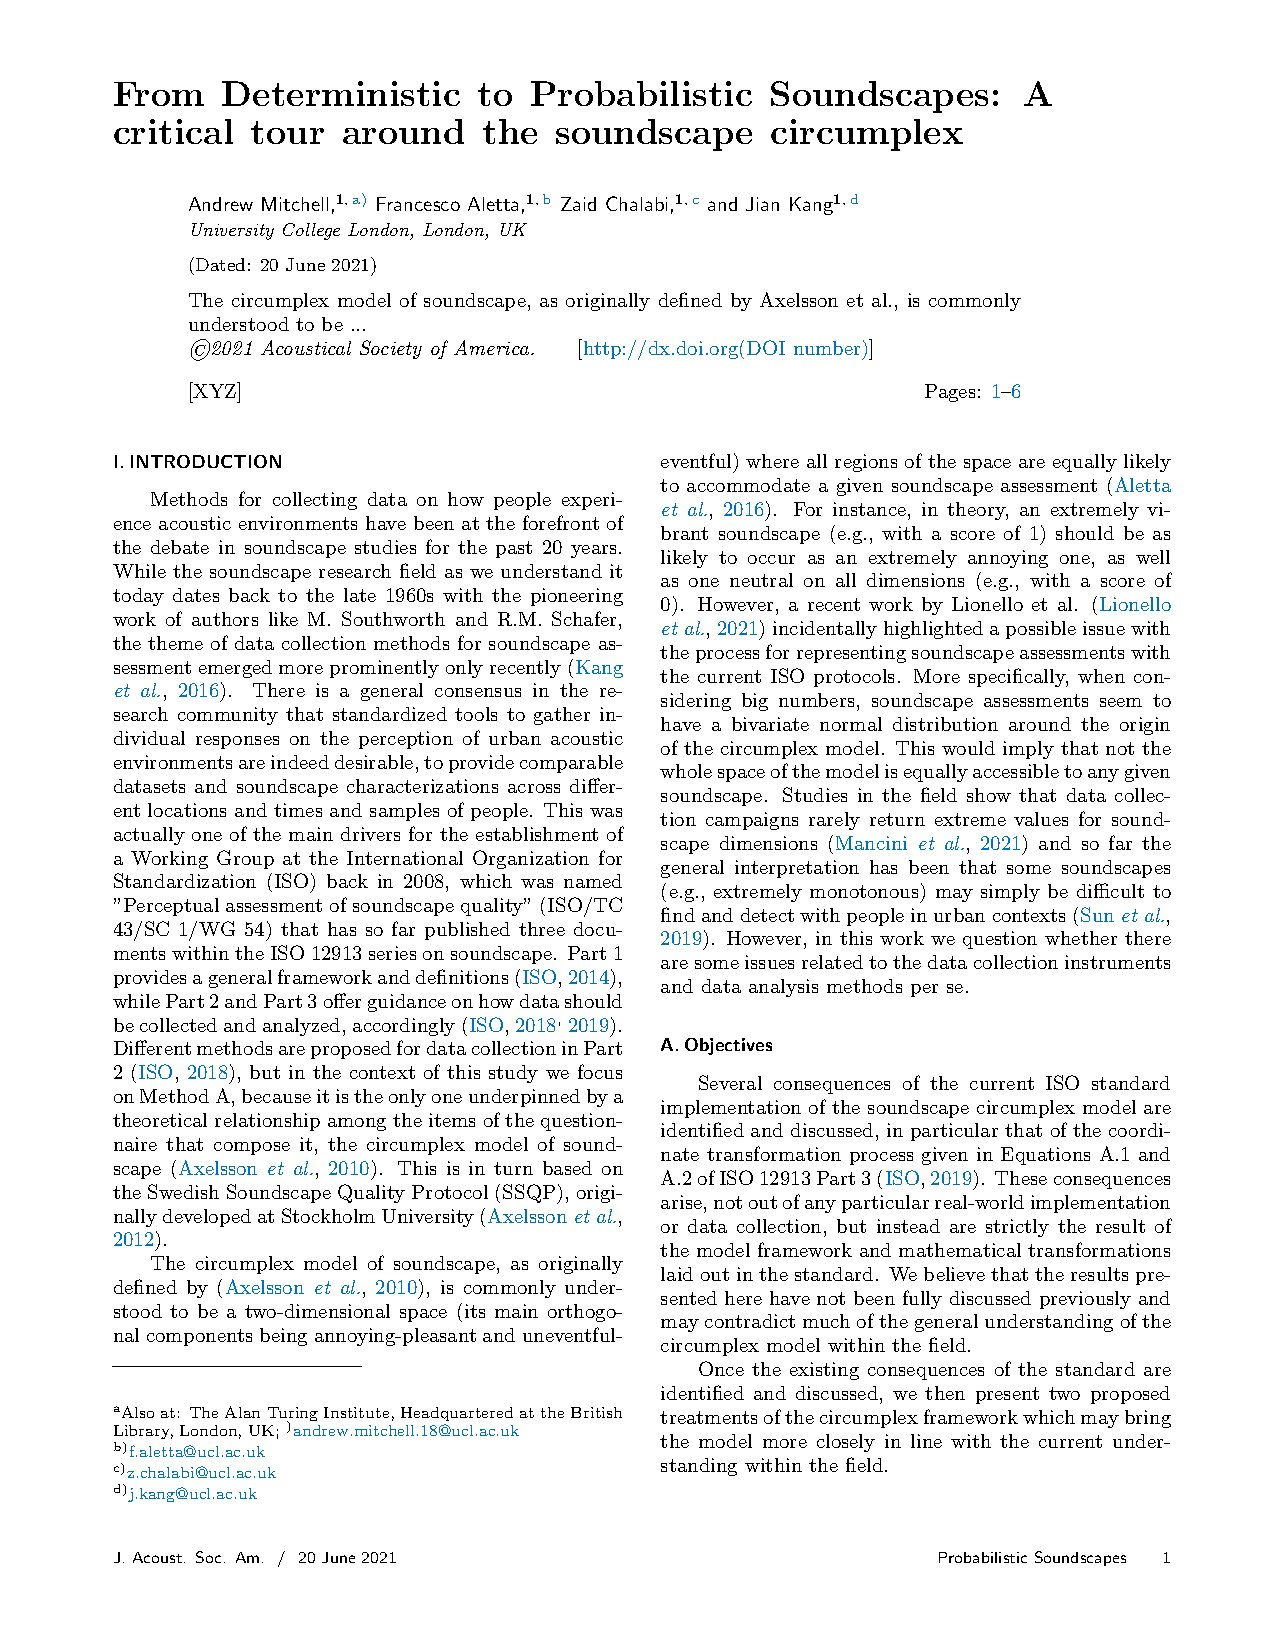
\includepdf[pages=-]{./Papers/J13_Circumplex_transform_Preprint.pdf}


 %%%%%%%%%%%%%%%%%%%%%%%%%%%%%%%%%%%%%%%%%%%%%%%%%%%%%%%%%%%%%%%%%%%%%%%%%%%%%%%%%%%%%%%%%%%%%%%%%%


 \chapter{Conclusions}
\label{ch:conc}

\section{General Discussion}

\section{Developing a framework for sustainable soundscapes}

\subsection{Defining Sustainability}



\section{Implications}

\section{Limitations and Recommendations for Future Research}

\section{Concluding Remarks}


 %%%%%%%%%%%%%%%%%%%%%%%%%%%%%%%%%%%%%%%%%%%%%%%%%%%%%%%%%%%%%%%%%%%%%%%%%%%%%%%%%%%%%%%%%%%%%%%%%%


 \backmatter
 % A glossary and list of acronyms may go here
 % or may go in the front matter after the abstract.
 \printglossaries

 % The bibliography will go here.
 \bibliography{thesis_refs}


 %%%%%%%%%%%%%%%%%%%%%%%%%%%%%%%%%%%%%%%%%%%%%%%%%%%%%%%%%%%%%%%%%%%%%%%%%%%%%%%%%%%%%%%%%%%%%%%%%%

\end{document}
